\documentclass{report}
\usepackage[utf8]{inputenc}
\usepackage[a4paper, right=2.5cm, left=2.5cm, top=2cm, bottom=2cm]{geometry}
\usepackage{graphicx}
% \usepackage[french]{babel}

%\usepackage[default,scale=0.95]{opensans}
\usepackage{lmodern}
\usepackage[T1]{fontenc}
\usepackage{amssymb} %math
\usepackage{amsmath}
\usepackage{amsthm}
\usepackage{systeme}
\usepackage{fancyhdr}
\usepackage{hyperref}
\usepackage{float}
\usepackage{titling}
\usepackage{lipsum}
\usepackage{subcaption}
% \usepackage{subfig}

\renewcommand*\familydefault{\sfdefault} %% Only if the base font of the document is to be sans serif
\hypersetup{
    colorlinks=true,
    linkcolor=blue,
    filecolor=magenta,      
    urlcolor=cyan,
    pdftitle={RDFIA Report - A.Delefosse, C.Vin},
    % pdfpagemode=FullScreen,
    }
    \urlstyle{same} %\href{url}{Text}
    
    \theoremstyle{plain}% default
\newtheorem{thm}{Théorème}[section]
\newtheorem{lem}[thm]{Lemme}
\newtheorem{prop}[thm]{Proposition}
\newtheorem*{cor}{Corollaire}
%\newtheorem*{KL}{Klein’s Lemma}

\theoremstyle{definition}
\newtheorem{defn}{Définition}[section]
\newtheorem{exmp}{Exemple}[section]
% \newtheorem{xca}[exmp]{Exercise}

\theoremstyle{remark}
\newtheorem*{rem}{Remarque}
\newtheorem*{note}{Note}
%\newtheorem{case}{Case}

\title{Basics on deep learning for vision}

\author{Aymeric \textsc{Delefosse} \& Charles \textsc{Vin}}
\date{2023 -- 2024}

% Definition of \maketitle
\makeatletter         
\def\@maketitle{
    \begin{center}
        {\Huge \bfseries \sffamily \@title }\\[4ex] 
        {\Large  \@author}\\[4ex] 
        \@date\\[8ex]
        
\includegraphics[width=40cm]{../figs/sorbonne-science.pdf}
    \end{center}}
\makeatother

\fancyhead{}
\fancyhead[L]{RDFIA}\fancyhead[R]{DAC 2023 -- 2024}
\pagestyle{fancy}
\thispagestyle{plain}

\begin{document}

\begin{titlepage}
    \centering
    
    % Title
    \vspace*{\fill}
    \Huge \thetitle \par
    \vspace{2mm}
    \Large \textbf{Deep Learning Practical Work} \par
    \vspace{2mm}

    % Author
    \Large \theauthor \par
    \vspace{2mm}
    % Date
    \large \thedate \par
    
    \vfill
    
    
\includegraphics[width=0.3\textwidth]{../figs/sorbonne-science.pdf}
    
\end{titlepage}

\tableofcontents
\newpage

\chapter{Introduction to neural networks}
\section{Theorical Foundation}
\subsection{Supervised dataset}
\paragraph{1. $\bigstar$ What are the train, val and test sets used for?}
The training dataset is utilized to train the model, while the test dataset is employed to assess the model's performance on previously unseen data. Lastly, the validation set constitutes a distinct subset of the dataset employed for the purpose of refining and optimizing the model's hyperparameters.

\paragraph{2. What is the influence of the number of exemples $N$?}
A larger number of examples can enhance the model's capacity to generalize and improve its robustness against noise or outliers. Conversely, a smaller number of examples can make the model susceptible to overfitting. It is important to note that increasing the dataset size can also lead to an escalation in the computational complexity of the model training process.

\subsection{Network architecture}
\paragraph{3. Why is it important to add activation functions between linear transformations?}
Otherwise, we would simply be aggregating linear functions, resulting in a linear output. Activation functions introduce non-linearity to the network, enabling the model to capture and learn more intricate patterns than those achievable through linear transformations alone.

\paragraph{4. $\bigstar$ What are the sizes $n_x$, $n_h$, $n_y$ in the figure 1? In practice, how are these sizes chosen?}
\begin{itemize}
    \item $n_x = 2$ represents the input size (data dimension).
    \item $n_h = 4$ represents the hidden layer size, selected based on the desired complexity of features to be learned in the hidden layer. An excessively large size can result in overfitting.
    \item $n_y = 2$ represents the output size, determined according to the number of classes in $y$.
\end{itemize}

\paragraph{5. What do the vectors $\hat{y}$ and $y$ represent? What is the difference between these two quantities?}
$y \in \{0,1\}$ represents the ground truth, where the values are binary (0 or 1).
$\hat{y} \in [0,1]$ represents a probability-like score assigned to each class by the model. $\hat{y}$ reflects the model's level of confidence in its predictions for each class.

\paragraph{6. Why use a $\text{SoftMax}$ function as the output activation function?}
The reason for employing the SoftMax function is to transform $\tilde{y} \in \mathbb{R}$ into a probability distribution. While there are several methods to achieve this transformation, $\text{SoftMax}$ is a commonly utilized choice, especially in multi-class classification problems.

\paragraph{7. Write the mathematical equations allowing to perform the \textit{forward} pass of the neural network, i.e. allowing to successively produce $\hat{h}$, $ h $, $ \tilde{y} $, $ \hat{y} $, starting at $x$.}
Let $W_i$ and $b_i$ denote the parameters for layer $i$, $f_i(x) = x W_i ^T + b_i$ represent the linear transformation, and $g_i(x)$ be the activation function for layer $i$.

Calculate the weighted sum and activation for the first hidden layer:
\begin{align*}
    \tilde{h} & = f_0(x)         \\
    h         & = g_0(\tilde{h})
\end{align*}

Proceed to the output layer by computing the weighted sum and activation for the output layer:
\begin{align*}
    \tilde{y} & = f_1(h)         \\
    \hat{y}   & = g_1(\tilde{y})
\end{align*}

These equations describe the sequential steps involved in the forward pass of the neural network, ultimately producing the output $\hat{y}$ based on the input $x$.

\subsection{Loss function}
\paragraph{8. During training, we try to minimize the loss function. For cross entropy and squared error, how must the $ \hat{y}_i $  vary to decrease the global loss function $ \mathcal{L} $?}
Our aim is to minimize the loss function $\mathcal{L}$ to train a model effectively. To decrease cross-entropy loss, make $\hat{y}_i$ closer to 1 when $y_i$ is 1 and closer to 0 when $y_i$ is 0.

For the cross-entropy loss, $\hat{y}_i$ should vary in a way that makes it closer to the true target value $y_i$ for each data point. Specifically, when $y_i = 1$, $\hat{y}_i$ should be pushed towards 1. The closer $\hat{y}_i$ is to 1, the lower the loss. Conversely, when $y_i = 0$, $\hat{y}_i$ should be pushed towards 0. The closer $\hat{y}_i$ is to 0, the lower the loss.

For squared error loss, $\hat{y}_i$ should vary in a way that makes it closer to the true target value $y_i$ for each data point. The goal is to minimize the squared difference between $\hat{y}_i$ and $y_i$. This means that if $\hat{y}_i$ is greater than $y_i$, it should decrease, and if $\hat{y}_i$ is smaller than $y_i$, it should increase.

\paragraph{9. How are these functions better suited to classification or regression tasks?}
Cross-entropy loss is better suited for classification tasks for several reasons:

\begin{itemize}
    \item Cross-entropy loss is based on the negative logarithm of the predicted probability of the true class. This logarithmic nature amplifies errors when the predicted probability deviates from 1 (for the correct class) and from 0 (for incorrect classes), depicted in \Cref{fig:CELoss}. Consequently, it effectively penalizes misclassifications, making it particularly suitable for classification tasks. However, it is imperative that $\hat{y}$ remains within the range $[0, 1]$ for this loss to be effective.
    \item Cross-entropy loss is often used in conjunction with the SoftMax activation function in the output layer of neural networks for multi-class classification. The SoftMax function ensures that the predicted probabilities sum to 1, aligning perfectly with the requirements of the cross-entropy loss.
\end{itemize}

\begin{figure}[H]
    \centering
    \includegraphics*[width=0.6\textwidth]{figs/cross_entropy.png}
    \caption{}
    \label{fig:CELoss}
\end{figure}

On the other hand, Mean Squared Error serves a different role and is better suited for regression tasks:

\begin{itemize}
    \item MSE is ideal when dealing with $(y, \hat{y}) \in \mathbb{R}^2$ (as opposed to the bounded interval $[0, 1]$).
    \item MSE is advantageous due to its convexity, which simplifies optimization. However, it's important to note that it may not always be the best choice for every regression task, especially when dealing with outliers, as it can be sensitive to extreme values.
\end{itemize}

\subsection{Optimization algorithm}
\paragraph{10. What seem to be the advantages and disadvantages of the various variants of gradient descent between the classic, mini-batch stochastic and online stochastic versions? Which one seems the most reasonable to use in the general case?}
Gradient computation becomes computationally expensive as it scales with the number of examples included. However, including more examples enhances gradient exploration with precision and stability, analogous to the exploration-exploitation trade-off in reinforcement learning.

Classic gradient descent offers stability, particularly with convex loss functions, featuring deterministic and reproducible updates. Nonetheless, its stability may lead to getting trapped in local minima when dealing with non-convex loss functions. Additionally, it is computationally intensive, especially for large datasets, as it demands evaluating the gradient with the entire dataset in each iteration.

Mini-Batch Stochastic Gradient Descent (SGD) converges faster compared to classic gradient descent by updating model parameters with small, random data subsets (mini-batches). This stochasticity aids in escaping local minima and exploring the loss landscape more efficiently. However, it may introduce noise and oscillations.

On the other hand, Online Stochastic Gradient Descent offers extremely rapid updates, processing one training example at a time, making it suitable for streaming or large-scale online learning scenarios. However, its highly noisy updates can result in erratic convergence or divergence, necessitating careful learning rate tuning.

For training deep neural networks in the general case, mini-batch stochastic gradient descent is the most reasonable choice. It strikes a balance between the computational efficiency of classic gradient descent and the noise resilience and convergence speed of online SGD.

\paragraph{11. $\bigstar$ What is the influence of the \textit{learning rate} $\eta$  on learning?}
The learning rate plays a crucial role in influencing various aspects of the learning process, including convergence speed, stability, and the quality of the final model.

A higher learning rate typically results in faster convergence because it leads to larger updates in model parameters during each iteration. However, an excessively high learning rate can cause issues such as overshooting, where the optimization process diverges or oscillates around the minimum, preventing successful convergence.

Conversely, a smaller learning rate allows the optimization algorithm to take smaller steps, which can be advantageous for exploring local minima more thoroughly and escaping shallow local minima. Nonetheless, if the learning rate is too small, it may lead to slow convergence or getting stuck in local minima.

To address these challenges, various techniques like learning rate schedules (gradually reducing the learning rate over time) or adaptive learning rate methods (e.g., Adam) have been developed to automate learning rate adjustments during training. The choice of learning rate may also be influenced by the batch size used in mini-batch stochastic gradient descent, as smaller batch sizes may require smaller learning rates to maintain stability.

In practice, selecting an appropriate learning rate often involves experimentation and can be problem-specific. Techniques such as grid search or random search, in combination with cross-validation, can aid in determining an optimal learning rate for a particular task.

\paragraph{12. $\bigstar$ Compare the complexity (depending on the number of layers in the network) of calculating the gradients of the \textit{loss} with respect to the parameters, using the naive approach and the \textit{backprop} algorithm.}
The naive method involves calculating the gradient of the loss function with respect to each parameter independently. For a network with a large number of parameters, this is computationally expensive and inefficient, essentially repeating a substantial amount of calculation needlessly. The complexity becomes substantial as the number of layers (and, as a result, the number of parameters) increases. It becomes a combinatorial problem with a complexity is $ \mathcal{O}(n!) $ where $n$ is the number of layers.

On the other hand, backpropagation leverages the chain rule from calculus to efficiently calculate gradients, making it a much more efficient strategy. It breaks down the complex task of computing derivatives for a multi-stage function into smaller, more manageable steps. This approach significantly reduces the computational burden, especially for networks with a large number of interconnected layers and parameters. Its complexity is linear, $\mathcal{O}(n)$, making it a much more practical choice for training deep neural networks.

\paragraph{13. What criteria must the network architecture meet to allow such an optimization procedure?}
For the backpropagation algorithm to be applicable, several criteria must be met. First of all, each layer function, including the activation functions and the loss function, must be differentiable with respect to their parameters. This is crucial for calculating gradients during the training process. Furthermore, as backpropagation relies on the sequential flow of information from the input layer to the output layer, the network architecture should possess a feedforward, sequential structure without loops or recurrent connections. Loops or recurrent connections can introduce complications in gradient calculations.

\paragraph{14. The function SoftMax and the \textit{loss} of \textit{cross-entropy} are often used together and their gradient is very simple. Show that the \textit{loss} can be simplified by:
    \[l = - \sum_{i}^{} y_i \tilde{y}_i + \log_{} \left(\sum_{i}^{} e^{\tilde{y}_i}\right)\]}
Let us define the cross-entropy loss as \( l(y, \hat{y}) = - \sum_{i=1}^{D} y_i \log \hat{y}_i \), where \( D \) represents the total number of classes. The SoftMax function for a vector \( \tilde{y} \in \mathbb{R}^D \) is defined as \( \text{SoftMax}(\tilde{y_i}) = \frac{e^{\tilde{y_i}}}{\sum_{j=1}^{D} e^{\tilde{y_j}}} \). Notably, the output of the SoftMax function serves as the input for the cross-entropy loss, denoted as \( \hat{y}_i = \text{SoftMax}(\tilde{y_i}) \). Let us substitute this value into the expression.

\begin{align*}
    l(y, \hat{y}) & = - \sum_{i=1}^{D} y_i \log_{} \hat{y}_i                                                                 \\
                  & = - \sum_{i=1}^{D} y_i \log_{} \text{SoftMax}(\tilde{y_i})                                               \\
                  & = - \sum_{i=1}^{D} y_i \log_{} \frac{e^{\tilde{y_i}}}{\sum_{j=1}^{D} e^{\tilde{y_j}} }                   \\
                  & = - \sum_{i=1}^{D} y_i \left[ \log_{} e^{\tilde{y}_i} - \log_{} \sum_{j=1}^{D} e^{\tilde{y}_j}  \right]  \\
                  & = - \sum_{i=1}^{D} y_i \tilde{y}_i - y_i \log_{} \sum_{j=1}^{D}e^{\tilde{y}_j}                           \\
                  & = - \sum_{i=1}^{D} y_i \tilde{y}_i + \sum_{i=1}^{D} y_i \log_{} \left(\sum_{j}^{D}e^{\tilde{y}_j}\right) \\
                  & = - \sum_{i=1}^{D} y_i \tilde{y}_i + \log_{} \left(\sum_{j}^{D}e^{\tilde{y}_j}\right) \sum_{i=1}^{D} y_i
\end{align*}

Since $y_i$ is one-hot encoded, we know that $\sum_i y_i = 1$. Thus, we have the final expression for the cross-entropy loss:

\[ l(y, \hat{y}) = - \sum_{i}^{} y_i \tilde{y}_i + \log_{} \left(\sum_{i}^{} e^{\tilde{y}_i}\right) \]

\paragraph{15. Write the gradient of the \textit{loss} (\textit{cross-entropy}) relative to the intermediate output $ \tilde{y} $ }
\begin{align*}
    \frac{\partial l}{\partial \tilde{y}_i} & = -y_i + \frac{\frac{\partial }{\partial \tilde{y}_i } (\sum_{j=1}^{D} e^{ \tilde{y}_j })}{\sum_{j=1}^{D} e^{ \tilde{y}_j }} \\
                                            & = - y_i + \frac{e^{\tilde{y}_i}}{\sum_{j=1}^{n_y} e^{ \tilde{y}_j}}                                                          \\
                                            & = - y_i + \text{SoftMax}(\tilde{y})_i
\end{align*}
\[
    \nabla _{\tilde{y}}l = \begin{pmatrix}
        \frac{\partial l}{\partial \tilde{y}_1} \\
        \vdots                                  \\
        \frac{\partial l}{\partial \tilde{y}_{n_y}}
    \end{pmatrix} = \begin{pmatrix}
        \text{SoftMax}(\tilde{y})_1 - y_1 \\
        \vdots                            \\
        \text{SoftMax}(\tilde{y})_{n_y} - y_{n_y}
    \end{pmatrix} \\
    = \hat{y} - y
\]

\paragraph{16. Using the \textit{backpropagation}, write the gradient of the \textit{loss} with respect to the weights of the output layer $ \nabla _{W_y}l $ . Note that writing this gradient uses $ \nabla _{\tilde{y}}l $ . Do the same for $ \nabla _{b_y}l $.}

Starting with \( \nabla _{W_y} l \), we have:

\[
    \frac{\partial l}{\partial W_{y,ij}} = \sum_{k}^{} \frac{\partial l}{\partial \tilde{y}_k} \frac{\partial \tilde{y}_k}{\partial W_{y,ij}}
\]

This can be expressed as a matrix:

\[
    \nabla_{W_y} l = \begin{pmatrix}
        \frac{\partial l}{\partial W_{y, 1,1}}   & \dots  & \frac{\partial l}{\partial W_{y, 1,n_h}}    \\
        \vdots                                   & \ddots & \vdots                                      \\
        \frac{\partial l}{\partial W_{y, n_y,1}} & \dots  & \frac{\partial l}{\partial W_{y, n_y, n_h}}
    \end{pmatrix}
\]

First, let's compute $ \tilde{y}_k $
\begin{align*}
    \tilde{y}   & = h W_y^T + b^y                                                                                                        \\
                & = \begin{pmatrix}
        h_{1} & \dots & h_{n_h}
    \end{pmatrix} * \begin{pmatrix}
        W_{1, 1}   & \dots  & W_{1, n_y}   \\
        \vdots     & \ddots & \vdots       \\
        W_{n_h, 1} & \dots  & W_{n_h, n_y} \\
    \end{pmatrix} + \begin{pmatrix}
        b^y_1 & \dots & b^y_{n_y}
    \end{pmatrix}                                 \\
                & = \begin{pmatrix}
        \sum_{j=1}^{n_h} W^y_{1,j} h_{j} + b^y_1 & \sum_{j=1}^{n_h} W^y_{2,j} h_{j} + b^y_2 & \dots & \sum_{j=1}^{n_h} W^y_{n_h,j} h_{k,j} + b^y_{n_h}
    \end{pmatrix}                                                           & \in \mathbb{R}^{1 \times n_h} \\
    \tilde{y}_k & = \sum_{j=1}^{n_h} W^y_{k,j} h_{j} + b_k^y, k \in [1, n_h]
\end{align*}

With this expression, we can now proceed with the calculation of the partial derivative of \( \tilde{y}_k \) with respect to \( W^y_{ij} \):

\[
    \frac{\partial \tilde{y}_k }{\partial W^y_{ij}} = \begin{cases}
        h_j & \text{ if } i=k   \\
        0   & \text{ otherwise}
    \end{cases}
\]

Now, we need to find \( \frac{\partial l}{\partial \tilde{y}_k} \). From the previous question, we have:

\[
    \frac{\partial l}{\partial \tilde{y}_k} = -y_k + \text{SoftMax}(\tilde{y})_k = \hat{y}_k - y_k
\]

Now, combining these results:

\[
    \frac{\partial l}{\partial W_{i,j}^y} = \sum_{k=1}^{n_h} \frac{\partial l}{\partial \tilde{y}_k} \frac{\partial \tilde{y}_k}{\partial W_{i,j}^y} =  \frac{\partial l}{\partial \tilde{y}_i} \frac{\partial \tilde{y}_i}{\partial W_{i,j}^y} = (\hat{y}_i - y_i) h_j = (\nabla _{W_y} l)_{i,j}
\]

So, the gradient of the loss with respect to the weights of the output layer \( \nabla_{W_y} l \) is given by \( \nabla _{\tilde{y}} ^T h \).

\begin{align*}
    \nabla_{W_y} l & = \begin{pmatrix}
        \frac{\partial l}{\partial W^y_{1,1}}   & \dots  & \frac{\partial l}{\partial W^y_{1,n_h}}    \\
        \vdots                                  & \ddots & \vdots                                     \\
        \frac{\partial l}{\partial W^y_{n_y,1}} & \dots  & \frac{\partial l}{\partial W^y_{n_y, n_h}}
    \end{pmatrix}                            \\
                   & = \begin{pmatrix}
        (\hat{y}_1 - y_1) h_{1}         & \dots  & (\hat{y}_1 - y_1) h_{n_h}         \\
        \vdots                          & \ddots & \vdots                            \\
        (\hat{y}_{n_y} - y_{n_y}) h_{1} & \dots  & (\hat{y}_{n_y} - y_{n_y}) h_{n_h}
    \end{pmatrix}                            \\
                   & = \begin{pmatrix}
        \hat{y}_1 - y_1 \\
        \vdots          \\
        \hat{y}_{n_y} - y_{n_y}
    \end{pmatrix} \begin{pmatrix}
        h_1 & h_2 & \dots & h_{n_h}
    \end{pmatrix} \\
                   & = \nabla _{\tilde{y}} ^T h
\end{align*}


% For the gradient with respect to the biases of the output layer \( \nabla_{b_y} l \), the calculation would be similar but would involve the derivative of \( \tilde{y}_k \) with respect to \( b_k^y \), which would be 1, and the gradient \( \frac{\partial l}{\partial \tilde{y}_k} \) remains the same. Putting it all together:

% \[
% \frac{\partial l}{\partial b_k^y} = \sum_{k=1}^{n_h} \frac{\partial l}{\partial \tilde{y}_k} \frac{\partial \tilde{y}_k}{\partial b_k^y} = (\hat{y}_k - y_k) \cdot 1 = \hat{y}_k - y_k
% \]

\paragraph{17. $\bigstar$ Compute other gradients : $ \nabla _{\tilde{h}} l, \nabla _{W_h} l, \nabla_{b_h}l $ }

\begin{enumerate}
    \item The gradient of the loss with respect to \( \tilde{h} \) can be computed using the chain rule:
          \[
              \frac{\partial l}{\partial \tilde{h}_i} = \sum_{k}^{} \frac{\partial l}{\partial h_k} \frac{\partial h_k}{\partial \tilde{h}_i}
          \]
          Let's compute those two terms:
          \[
              \frac{\partial h_k}{\partial \tilde{h}_i} = \frac{\partial \tanh (\tilde{h_k})}{\partial \tilde{h_i}} = \begin{cases}
                  1 - \tanh^2 (\tilde{h_i}) = 1 - h_i^2 & \text{ if } k = i \\
                  0                                     & \text{ otherwise} \\
              \end{cases}
          \]

          Having $ \tilde{y}_i = \sum_{j=1}^{n_h} W_{i,j}^y h_j +b_i^y$ in mind and recovering $ \frac{\partial l}{\partial \tilde{y}_i} = \hat{y}_i - y_i = \delta ^y_i $ from past question:
          \[
              \frac{\partial l}{\partial h_k} = \sum_{j=1}^{} \frac{\partial l}{\partial \tilde{y_j}} \frac{\partial \tilde{y}_j}{\partial h_k} = \sum_{j=1}^{} \delta ^y_j W^y_{j,k}
          \]

          Finally,
          \begin{align*}
              \frac{\partial l}{\partial \tilde{h}_i} & = \sum_{k}^{} \frac{\partial l}{\partial h_k} \frac{\partial h_k}{\partial \tilde{h}_i} \\
                                                      & = \sum_{k}^{} \sum_{j}^{} \delta ^y_j W^y_{j,k} \times \begin{cases}
                  1 - h_i^2 & \text{ if } k = i \\
                  0         & \text{ otherwise} \\
              \end{cases}       \\
                                                      & = (1 - h_i^2) \left(\sum_{j}^{} \delta ^y_j W^y_{j,i}\right)                            \\
                                                      & = \delta ^h _i
          \end{align*}
          So, the gradient \( \nabla _{\tilde{h}} l \) is a vector with elements $ \delta ^h _i $:

          \[
              \nabla _{\tilde{h}} l = (1 - h^2) \odot (\nabla _{\tilde{y}} l * W^y)
          \]


    \item $ \nabla _{W^h} l $ is a matrix composed of elements
          \[
              \frac{\partial l}{\partial W^h _{i,j}} = \sum_{k}^{} \frac{\partial l}{\partial \tilde{h}_k} \frac{\partial \tilde{h}_k}{\partial W^h_{i,j}}
          \]
          From the previous question, we already have $ \frac{\partial l}{\partial h_k} = (1 - h_k^2) (\sum_{j}^{} \delta ^y_j W^y_{j,k}) = \delta_k^h$. So let's compute the other term $ \frac{\partial \tilde{h}_k}{\partial W^h_{i,j}}  $ from $ \tilde{h}_k = \sum_{j=1}^{n_x} W^h_{k,j} x_j + b_k^h $

          \[
              \frac{\partial \tilde{h}_k}{\partial W^h_{i,j}} = \begin{cases}
                  x_j & \text{ if } k = i  \\
                  0   & \text{ otherwise } \\
              \end{cases}
          \]
          So:
          \begin{align*}
              \frac{\partial l}{\partial W^h _{i,j}} & = \sum_{k}^{} \frac{\partial l}{\partial \tilde{h}_k} \frac{\partial \tilde{h}_k}{\partial W^h_{i,j}} \\
                                                     & = \sum_{k}^{}\delta ^h_k \times \begin{cases}
                  x_j & \text{ if } k = i  \\
                  0   & \text{ otherwise } \\
              \end{cases}                                            \\
                                                     & = \delta _i^h x_j                                                                                     \\
              \nabla _W^h                            & = \nabla _{\tilde{h}} ^T l * x
          \end{align*}


    \item Last but not least:
          \[
              \frac{\partial l}{\partial b_i^j} = \sum_{k}^{} \frac{\partial l}{\partial \tilde{h}_k} \frac{\partial \tilde{h}_k}{\partial b_i^h} = \sum_{k}^{}\delta _k^h * \begin{cases}
                  1 & \text{ if } k = i \\
                  0 & \text{ else}      \\
              \end{cases} = \delta ^h_i
          \]

          \[
              \nabla _{b^h} = \nabla _{\tilde{h}} l
          \]

\end{enumerate}

\section{Implementation}

In this section, the primary focus was on exploring how a simple neural network model can perform at classifying tasks which can be difficult with normal machine learning techniques. The context varied from circular data to image classification, and the overall approach was to confirm the theory of precedent section and experiment with different hyperparameters to understand their effects on model performance.

\subsection{Forward and backward manuals}
In neural network training using SGD, it is common practice to average the gradients calculated during the backward pass over the batch size. The idea behind this scaling is to make the learning rate independent of the batch size, so that the updates to the model parameters are roughly consistent regardless of the batch size. We compared these two approaches in \Cref{fig:manual_nn}.

One significant observation is that when using batch normalization, the network requires much more time to achieve its performance, needing 100 epochs instead of 10. However, the trade-off is that the training process becomes much more stable.

\begin{figure}[H]
    \centering
    \begin{subfigure}{0.45\textwidth}
        \centering
        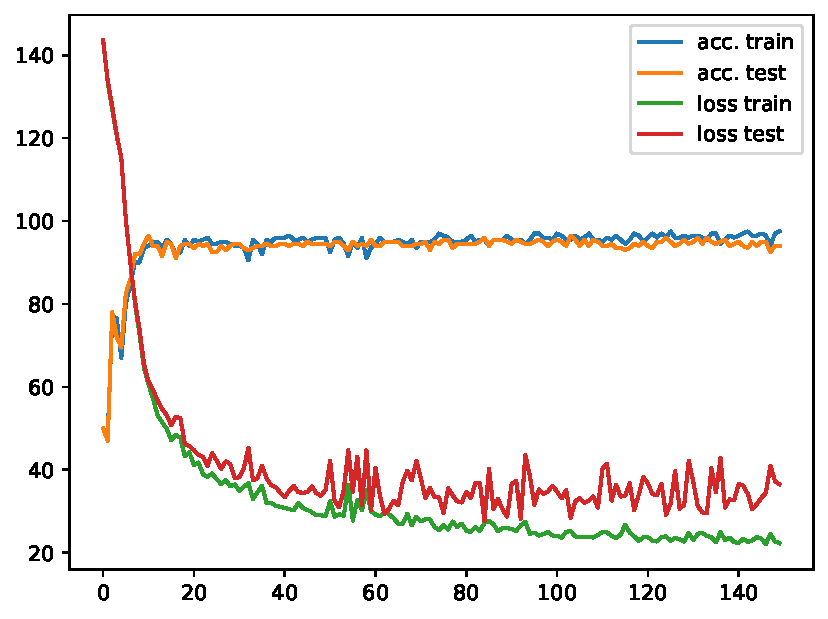
\includegraphics[width=\textwidth]{figs/NN/manual_acc_loss.pdf}
        \caption{Accuracy and losses curves without batch size normalization}
        \label{subfig:manual_acc_loss}
    \end{subfigure}
    \begin{subfigure}{0.45\textwidth}
        \centering
        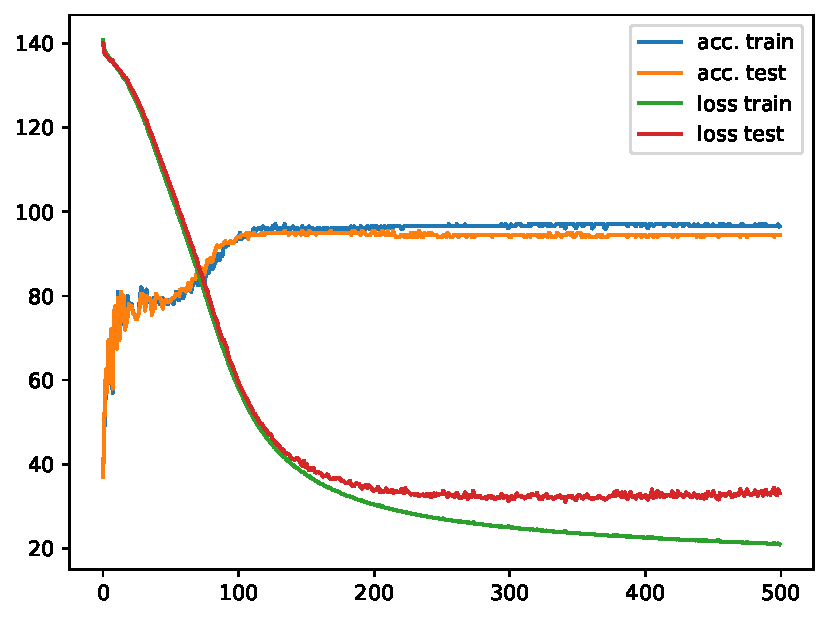
\includegraphics[width=\textwidth]{figs/NN/manual_acc_loss_bis.pdf}
        \caption{Accuracy and losses curves with batch size normalization}
        \label{subfig:manual_acc_loss_bis}
    \end{subfigure}
    \caption{To batch normalize, or not to batch normalize.}
    \label{fig:manual_nn}
\end{figure}

In the following experiments, we have chosen to continue with batch normalization. We then proceeded to investigate the influence of learning rate and batch size. The results are presented in \Cref{fig:manual_bs_lr}. Our findings align with the expectations discussed in Question 11.

\begin{figure}[H]
    \centering
    \begin{subfigure}{0.45\textwidth}
        \centering
        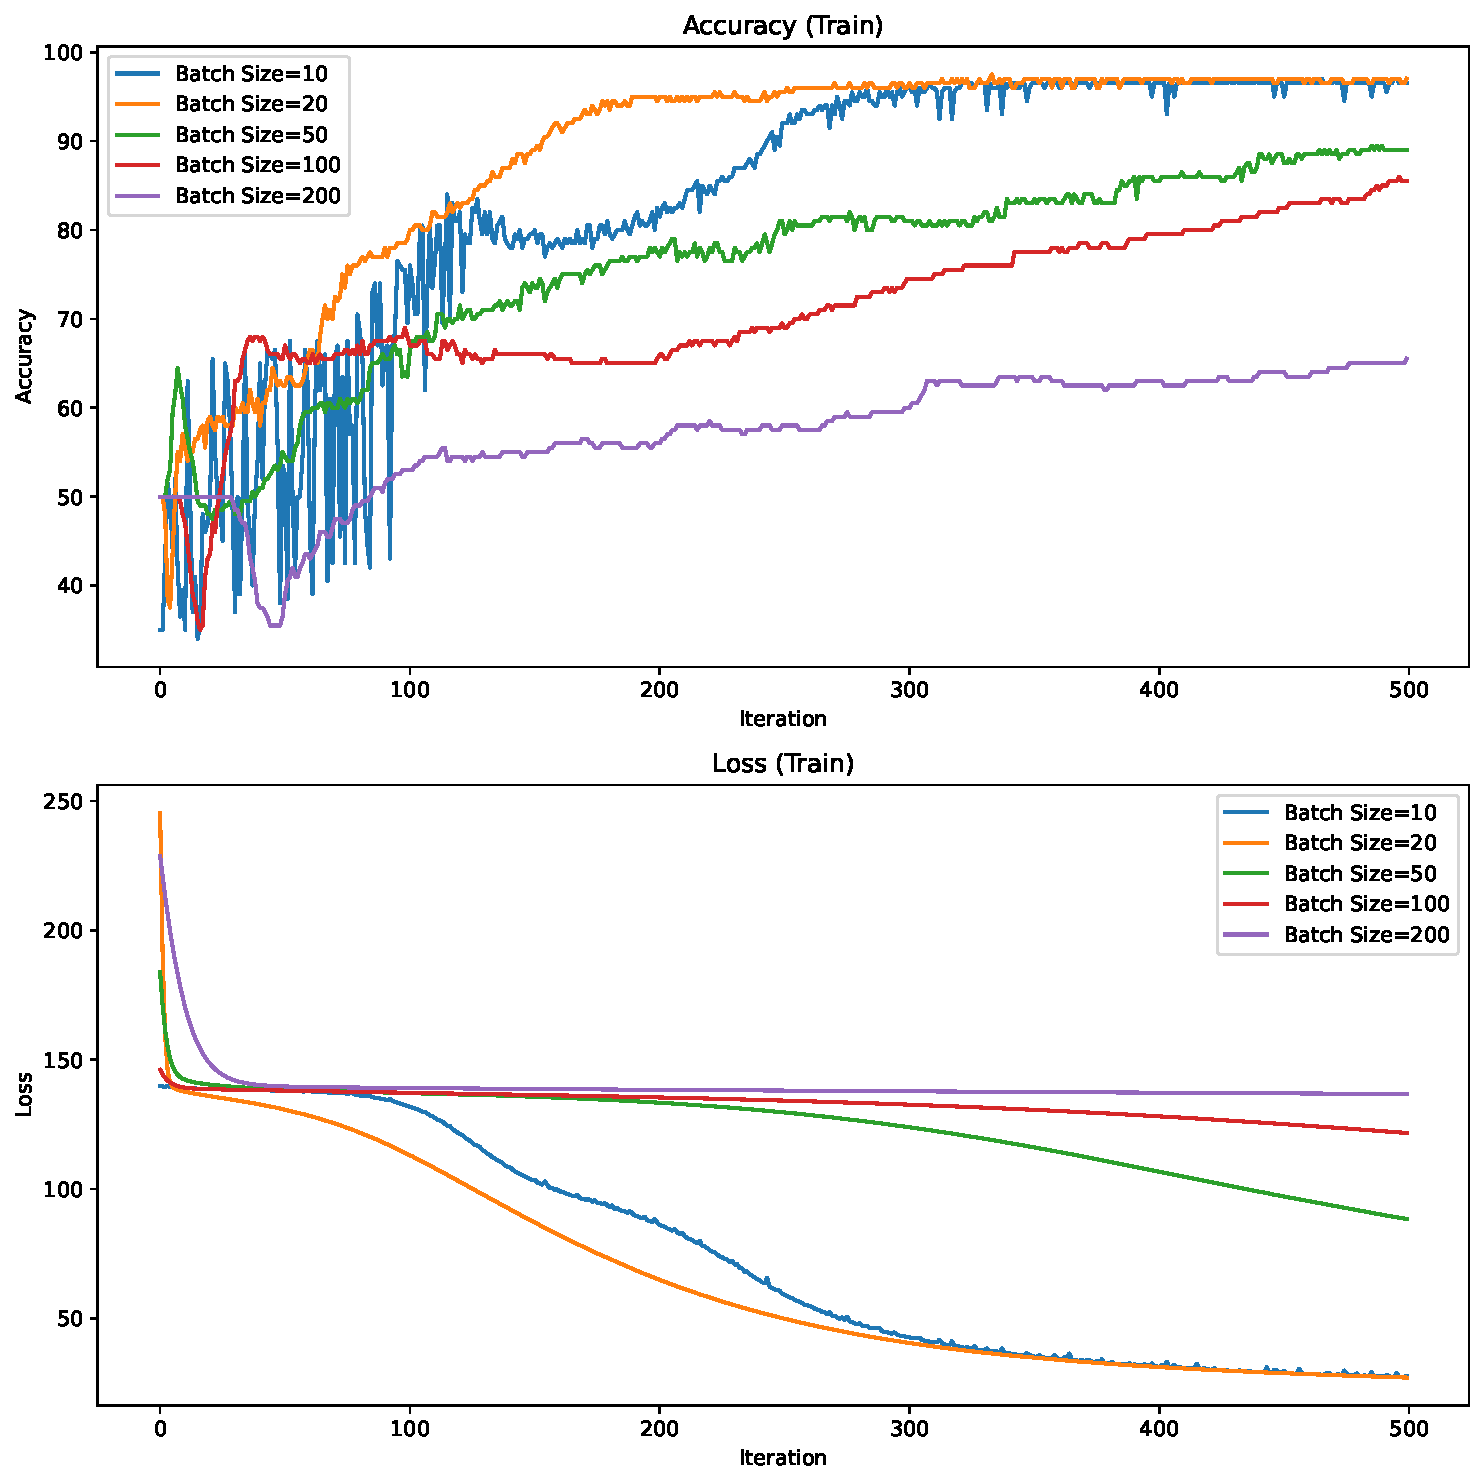
\includegraphics[width=\textwidth]{figs/NN/manual_batchsize.pdf}
        \caption{Influence of batch size}
        \label{subfig:manual_batchsize}
    \end{subfigure}
    \begin{subfigure}{0.45\textwidth}
        \centering
        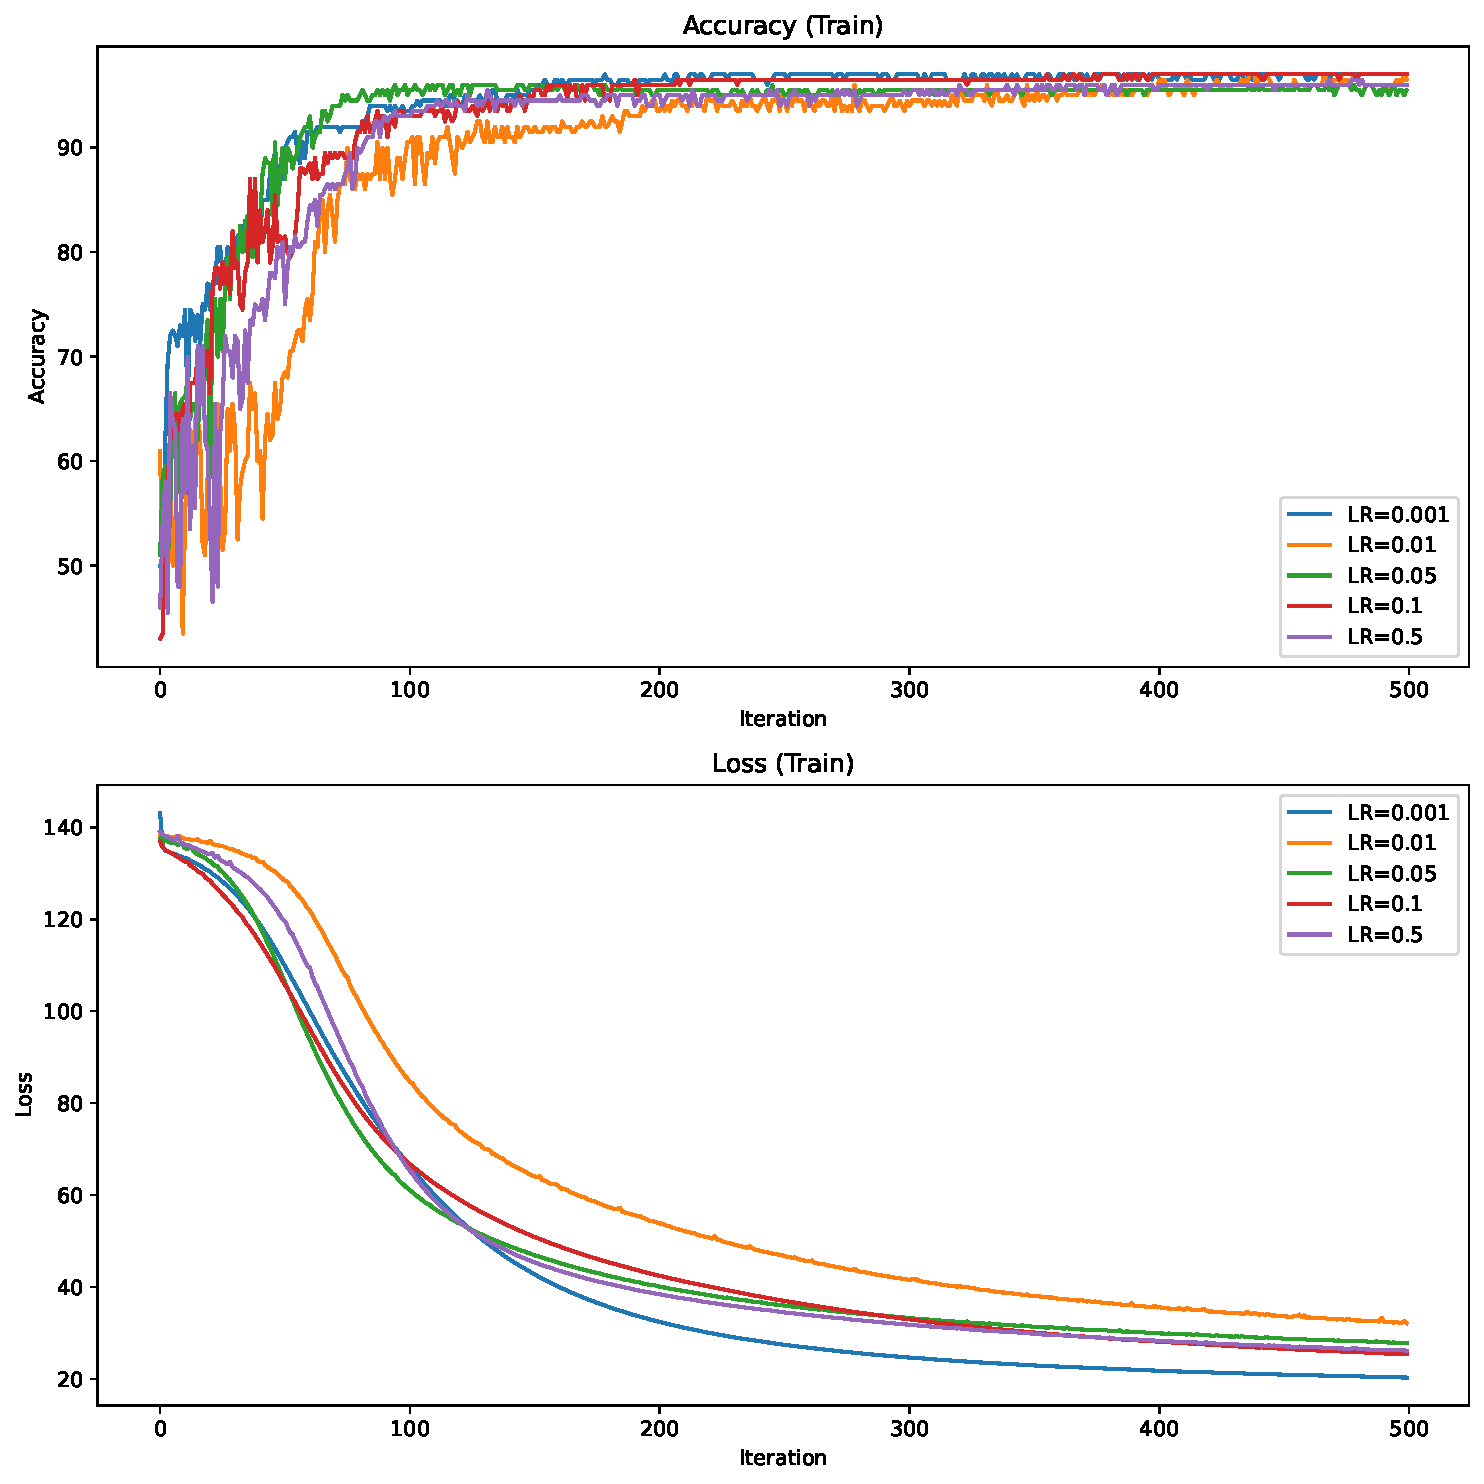
\includegraphics[width=\textwidth]{figs/NN/manual_lr.pdf}
        \caption{Influence of learning rate}
        \label{subfig:manual_lr}
    \end{subfigure}
    \caption{Influence of learning rate and batch size}
    \label{fig:manual_bs_lr}
\end{figure}

In the provided notebook, you will also find animated figures that showcase the evolution of the learning process and the visualization of the decision boundaries. Unexpectedly, by the end of the training, we can observe circular decision boundaries for the circular data as the model is able to classify the data correctly.

% \pagebreak
\subsection{Simplification of the backward pass with \texttt{torch.autograd}}

The results of this section are presented in \Cref{fig:autograd}. It's worth noting that we obtained similar results to when we did not use batch normalization, as indicated by the learning instability. However, our overall conclusions remain consistent.


\begin{figure}[H]
    \centering
    \begin{subfigure}{\textwidth}
        \centering
        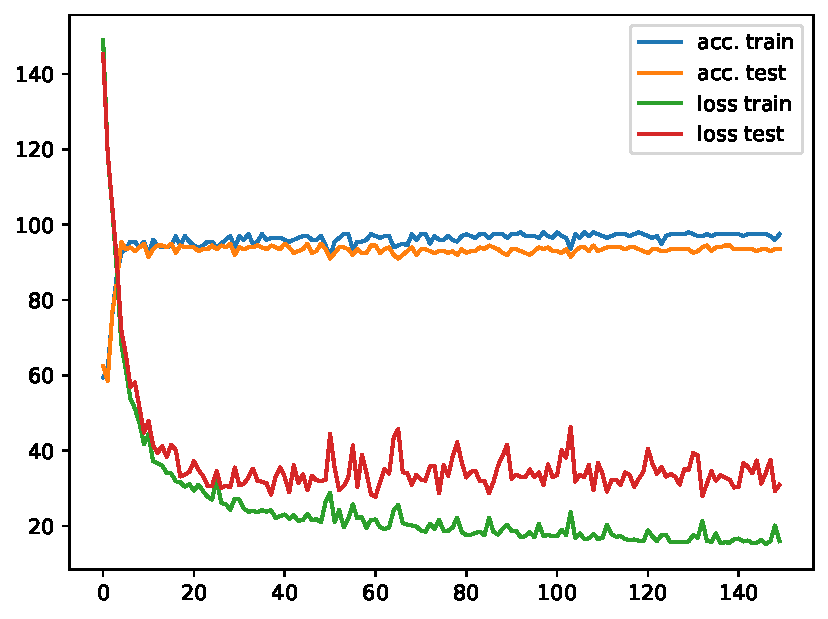
\includegraphics[width=0.5\textwidth, height=5cm]{figs/NN/autograd_acc_loss.pdf}
        \caption{Accuracy and losses curves with \texttt{torch.autograd}}
        \label{subfig:autograd_acc_loss}
    \end{subfigure}
\end{figure}

\begin{figure}[H]\ContinuedFloat
    \centering
    \begin{subfigure}{0.45\textwidth}
        \centering
        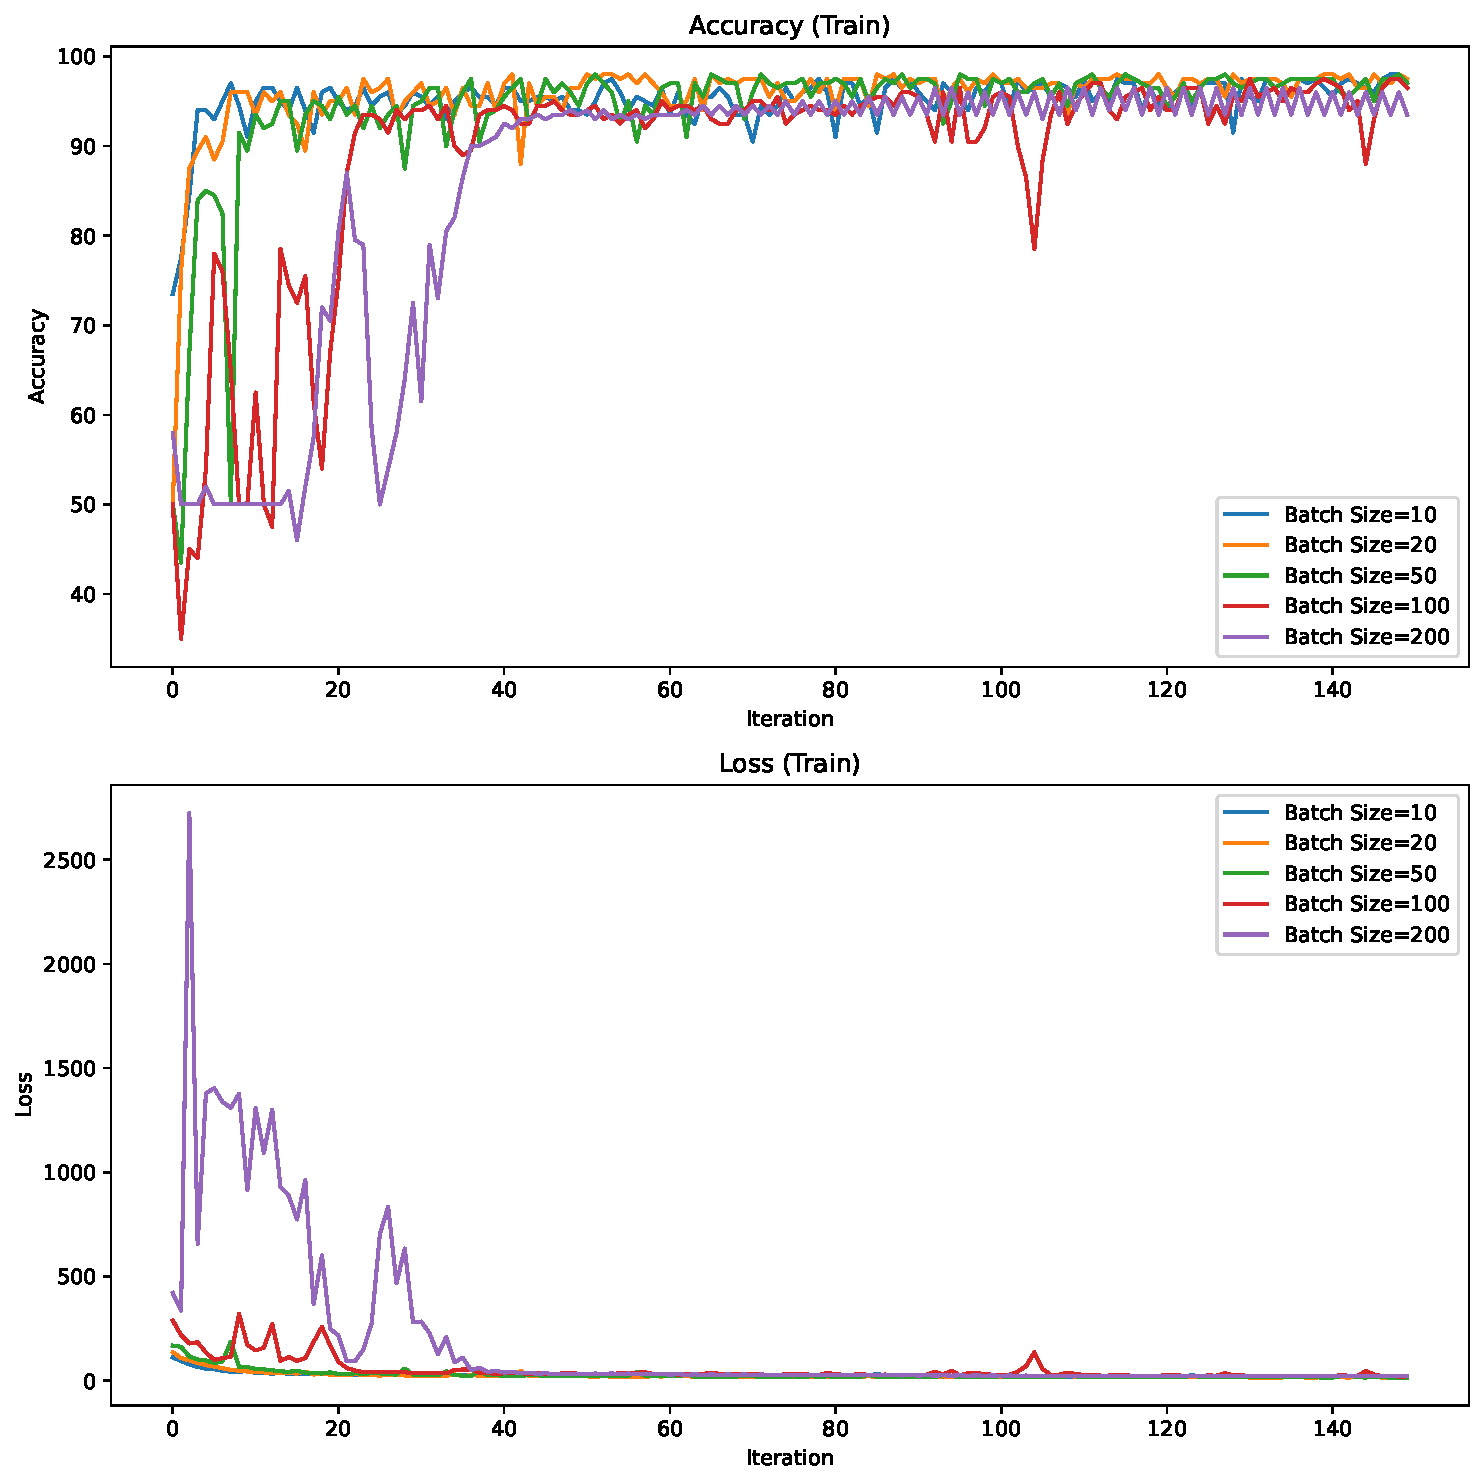
\includegraphics[width=\textwidth]{figs/NN/autograd_batchsize.pdf}
        \caption{Influence of batch size}
        \label{subfig:autograd_batchsize}
    \end{subfigure}
    \begin{subfigure}{0.45\textwidth}
        \centering
        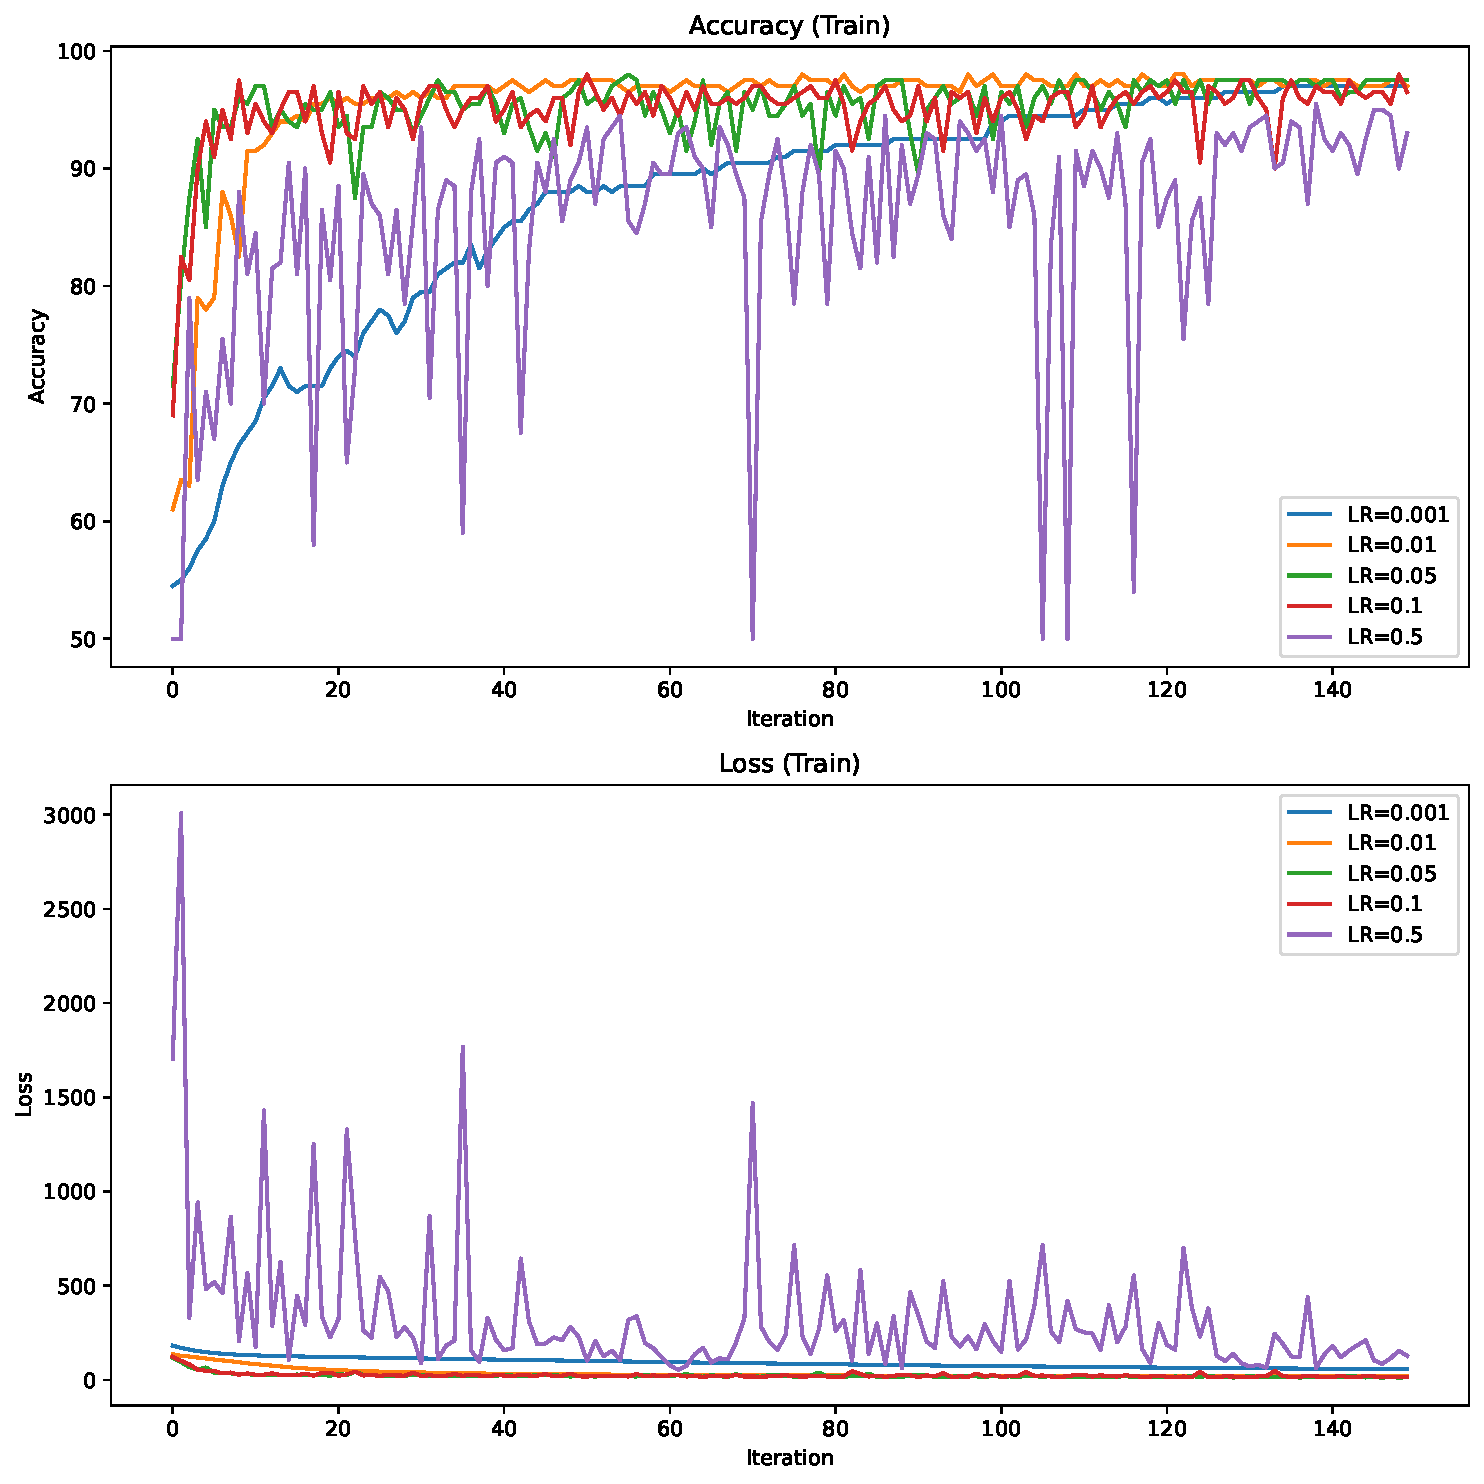
\includegraphics[width=\textwidth]{figs/NN/autograd_lr.pdf}
        \caption{Influence of learning rate}
        \label{subfig:autograd_lr}
    \end{subfigure}
    \caption{\texttt{torch.autograd}}
    \label{fig:autograd}
\end{figure}

\subsection{Simplification of the forward pass with \texttt{torch.nn} layers}

The results of this section can be found in \Cref{fig:torchnn}. In this case, we observe that learning takes longer compared to using manual layers. It requires 150 epochs to reach its maximum performance. This could be attributed to how Torch initializes its layers. However, the training process appears to be more stable, as evidenced by the loss curve.

\begin{figure}[H]
    \centering
    \begin{subfigure}{\textwidth}
        \centering
        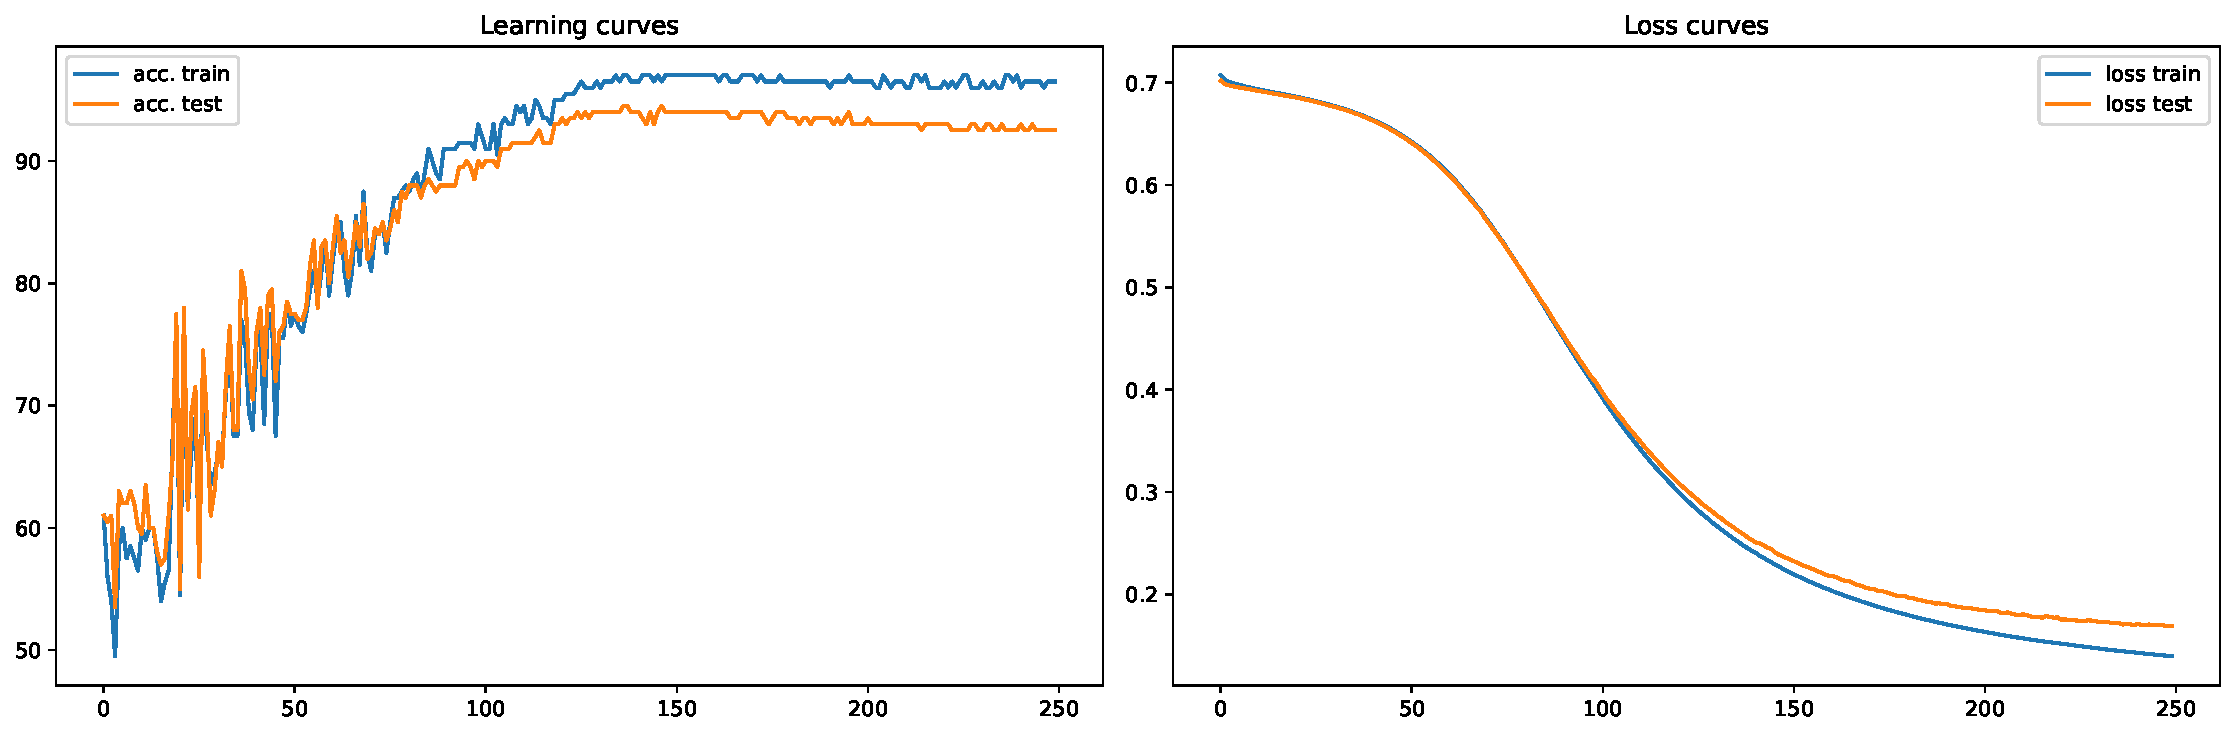
\includegraphics[width=0.88\textwidth]{figs/NN/torchnn_acc_loss.pdf}
        \caption{Accuracy and losses curves using \texttt{torch.nn} layers}
        \label{subfig:torchnn_acc_loss}
    \end{subfigure}
\end{figure}

\begin{figure}[H]\ContinuedFloat
    \centering
    \begin{subfigure}{0.45\textwidth}
        \centering
        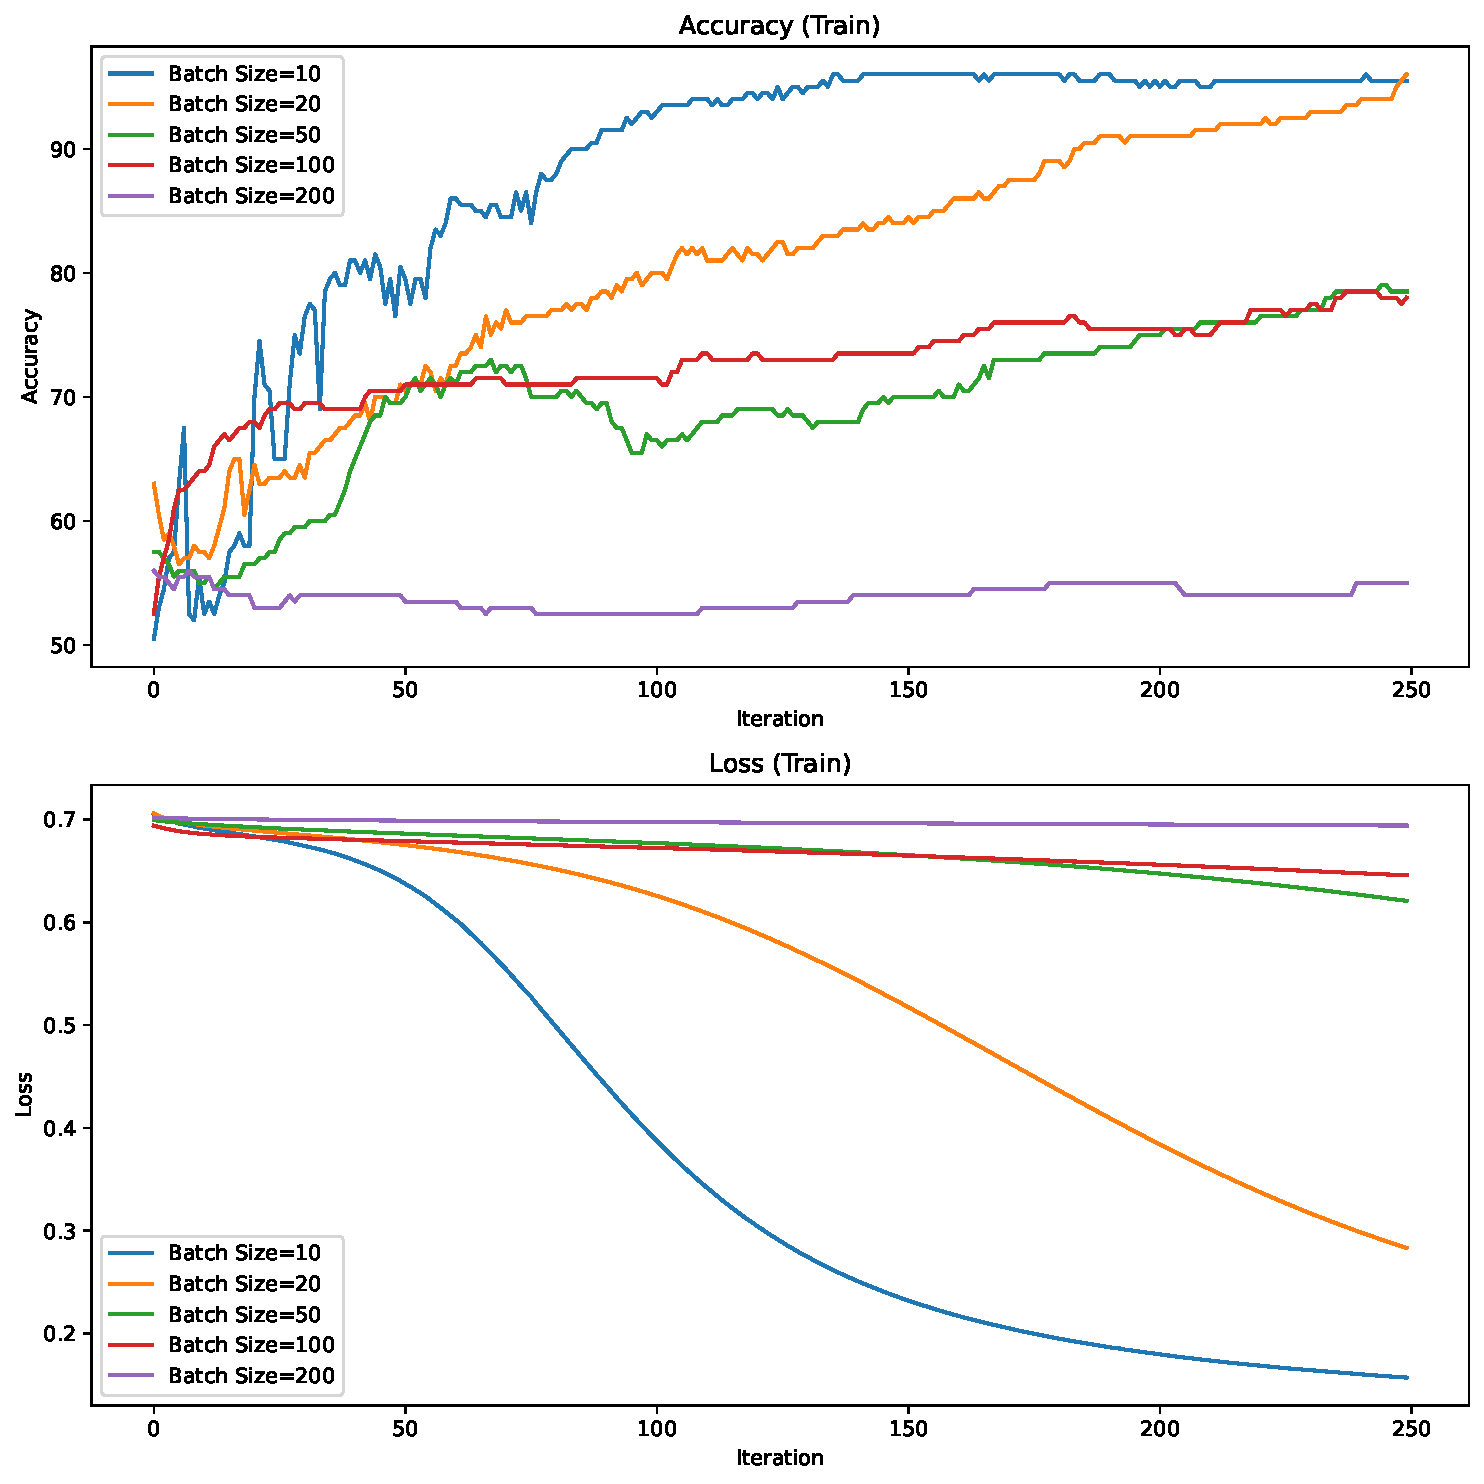
\includegraphics[width=\textwidth]{figs/NN/torchnn_batch_size.pdf}
        \caption{Influence of batch size}
        \label{subfig:torchnn_batchsize}
    \end{subfigure}
    \begin{subfigure}{0.45\textwidth}
        \centering
        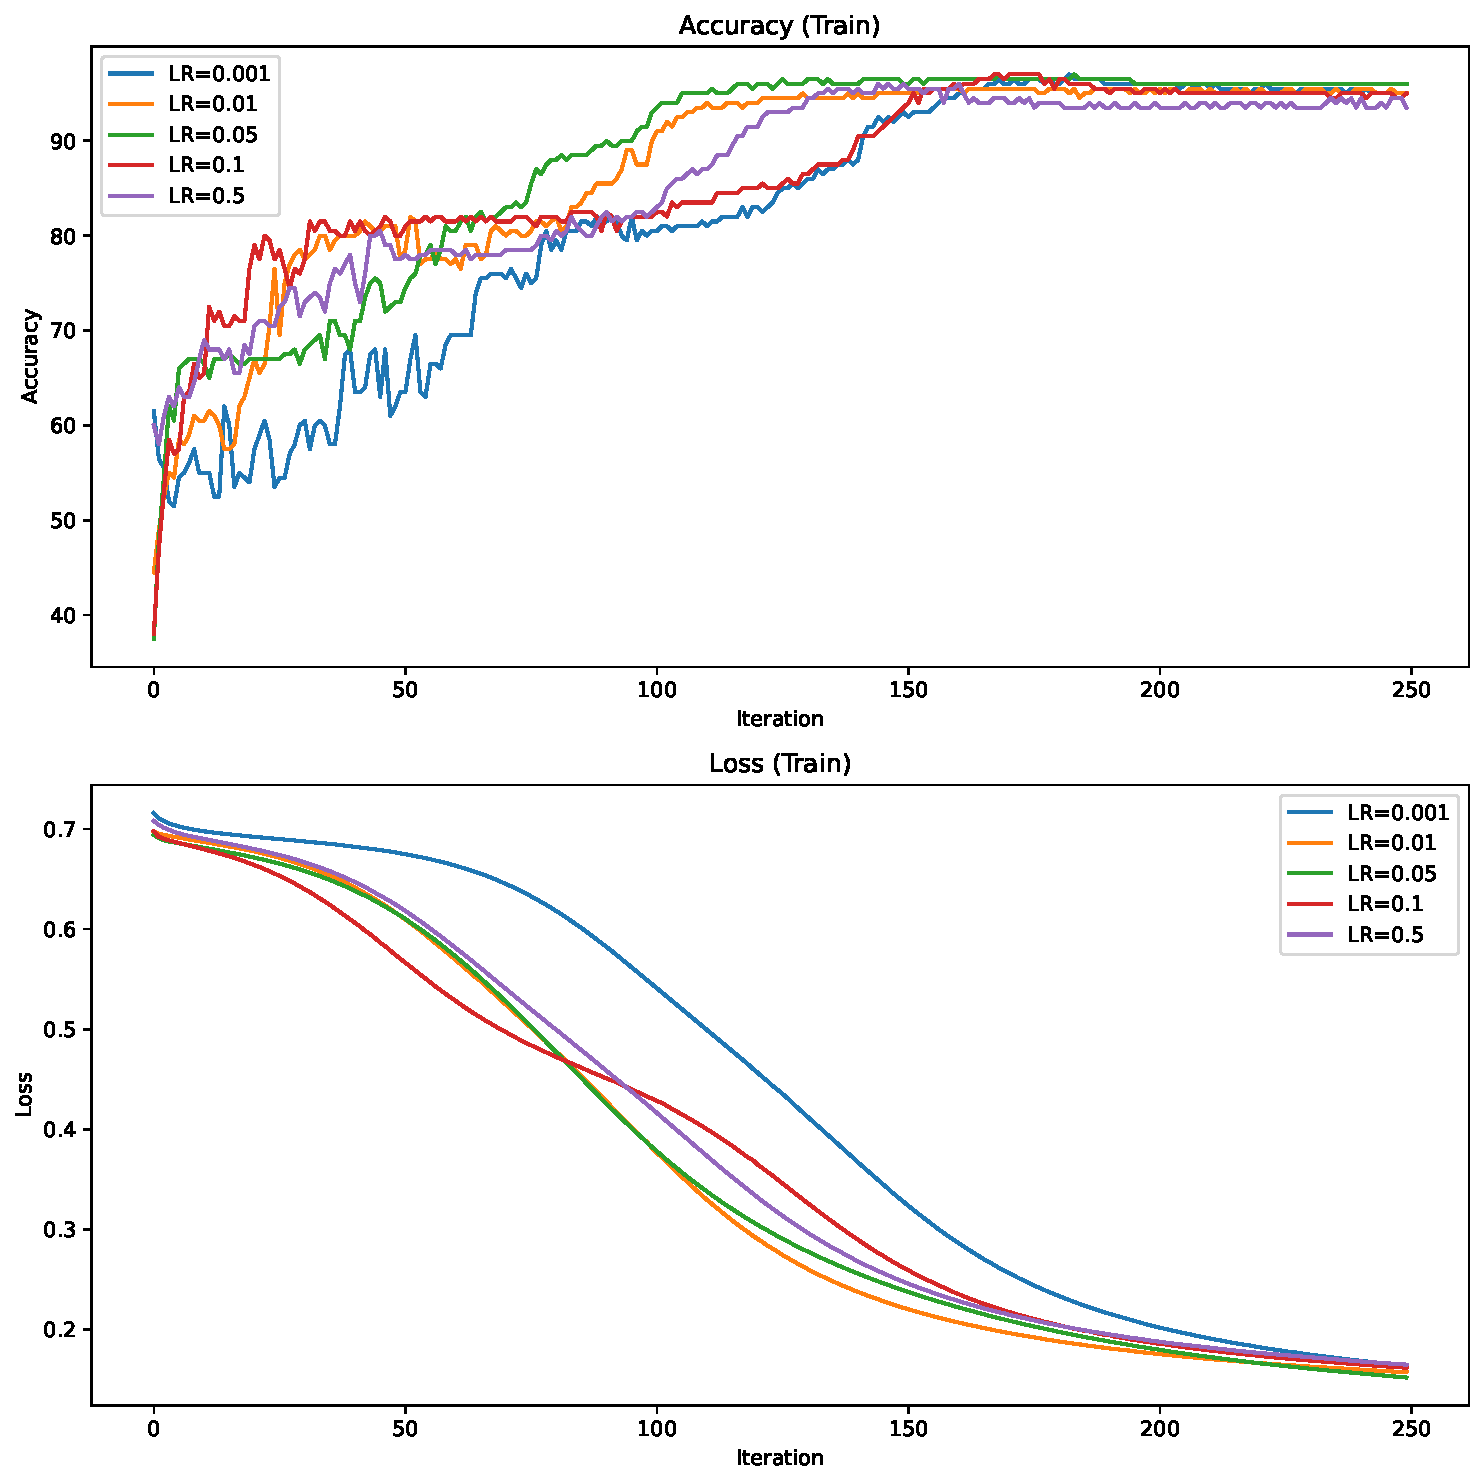
\includegraphics[width=\textwidth]{figs/NN/torchnn_lr.pdf}
        \caption{Influence of learning rate}
        \label{subfig:torchnn_lr}
    \end{subfigure}
    \caption{\texttt{torch.nn} }
    \label{fig:torchnn}
\end{figure}

\subsection{Simplification of the SGD with \texttt{torch.optim}}

The results of this section are presented in \Cref{fig:torchoptim}. The training process is significantly more stable, but it requires a much longer time to converge, taking 300 epochs to reach its maximum performance. 

\begin{figure}[H]
    \centering
    \begin{subfigure}{\textwidth}
        \centering
        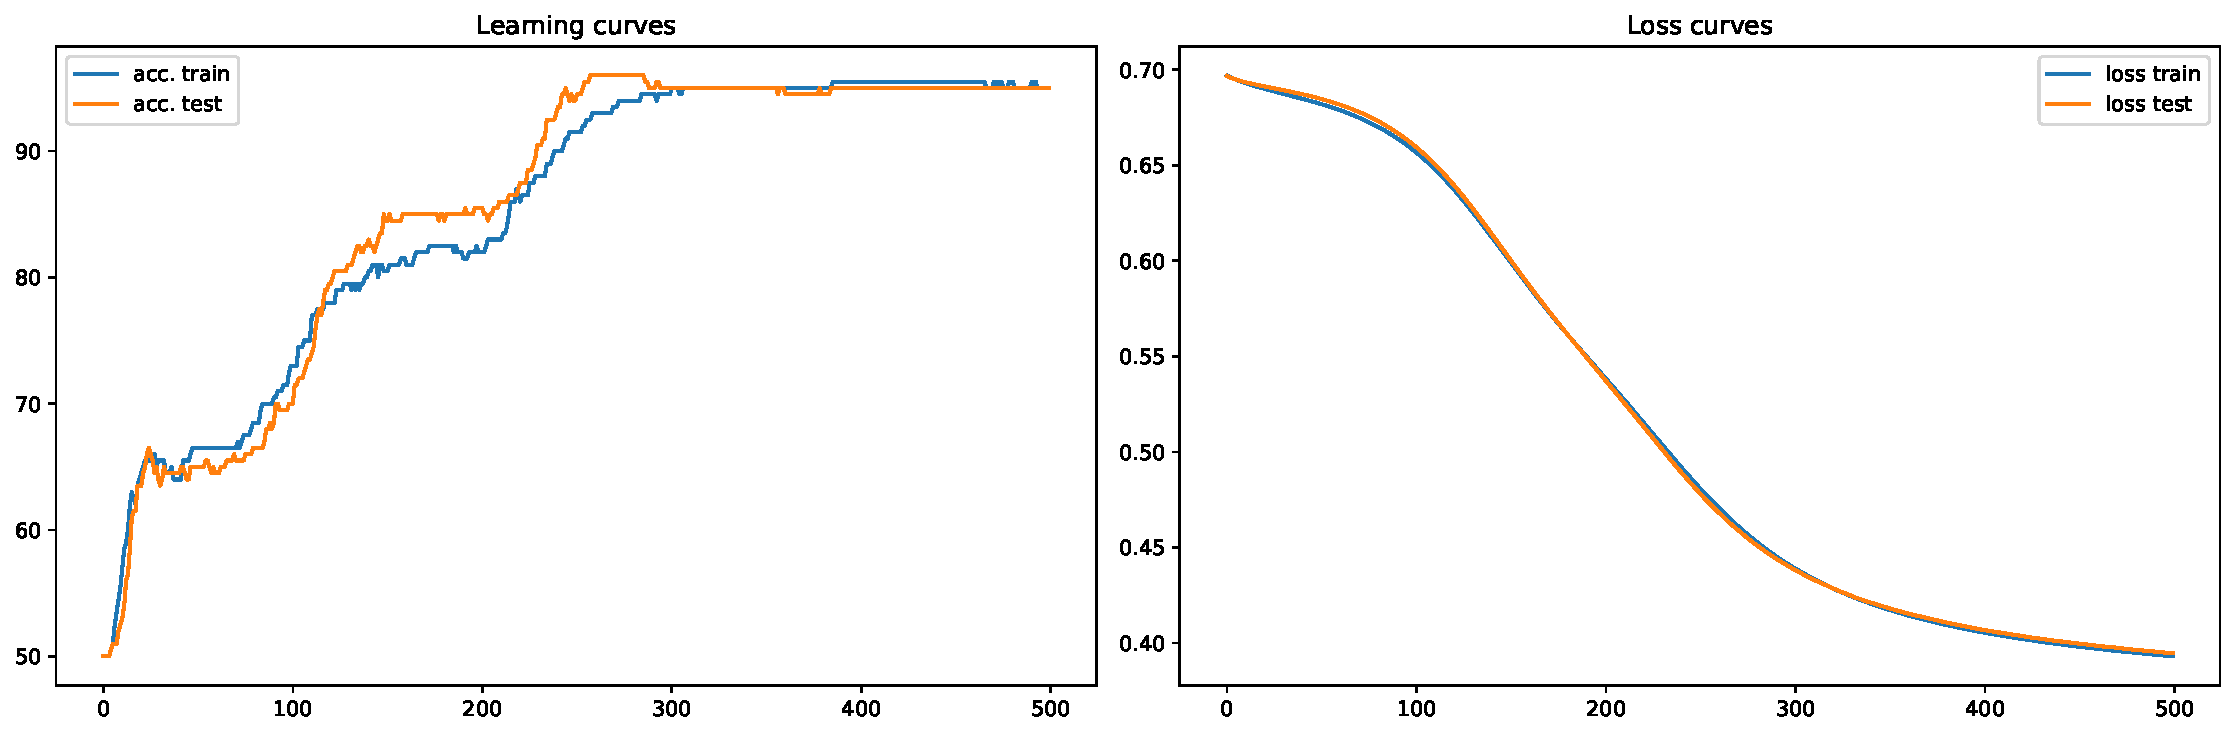
\includegraphics[width=0.88\textwidth]{figs/NN/torchoptim_acc_loss.pdf}
        \caption{Accuracy and losses curves using \texttt{torch.optim}}
        \label{subfig:torchoptim_acc_loss}
    \end{subfigure}
\end{figure}

\begin{figure}[H]\ContinuedFloat
    \centering
    \begin{subfigure}{0.45\textwidth}
        \centering
        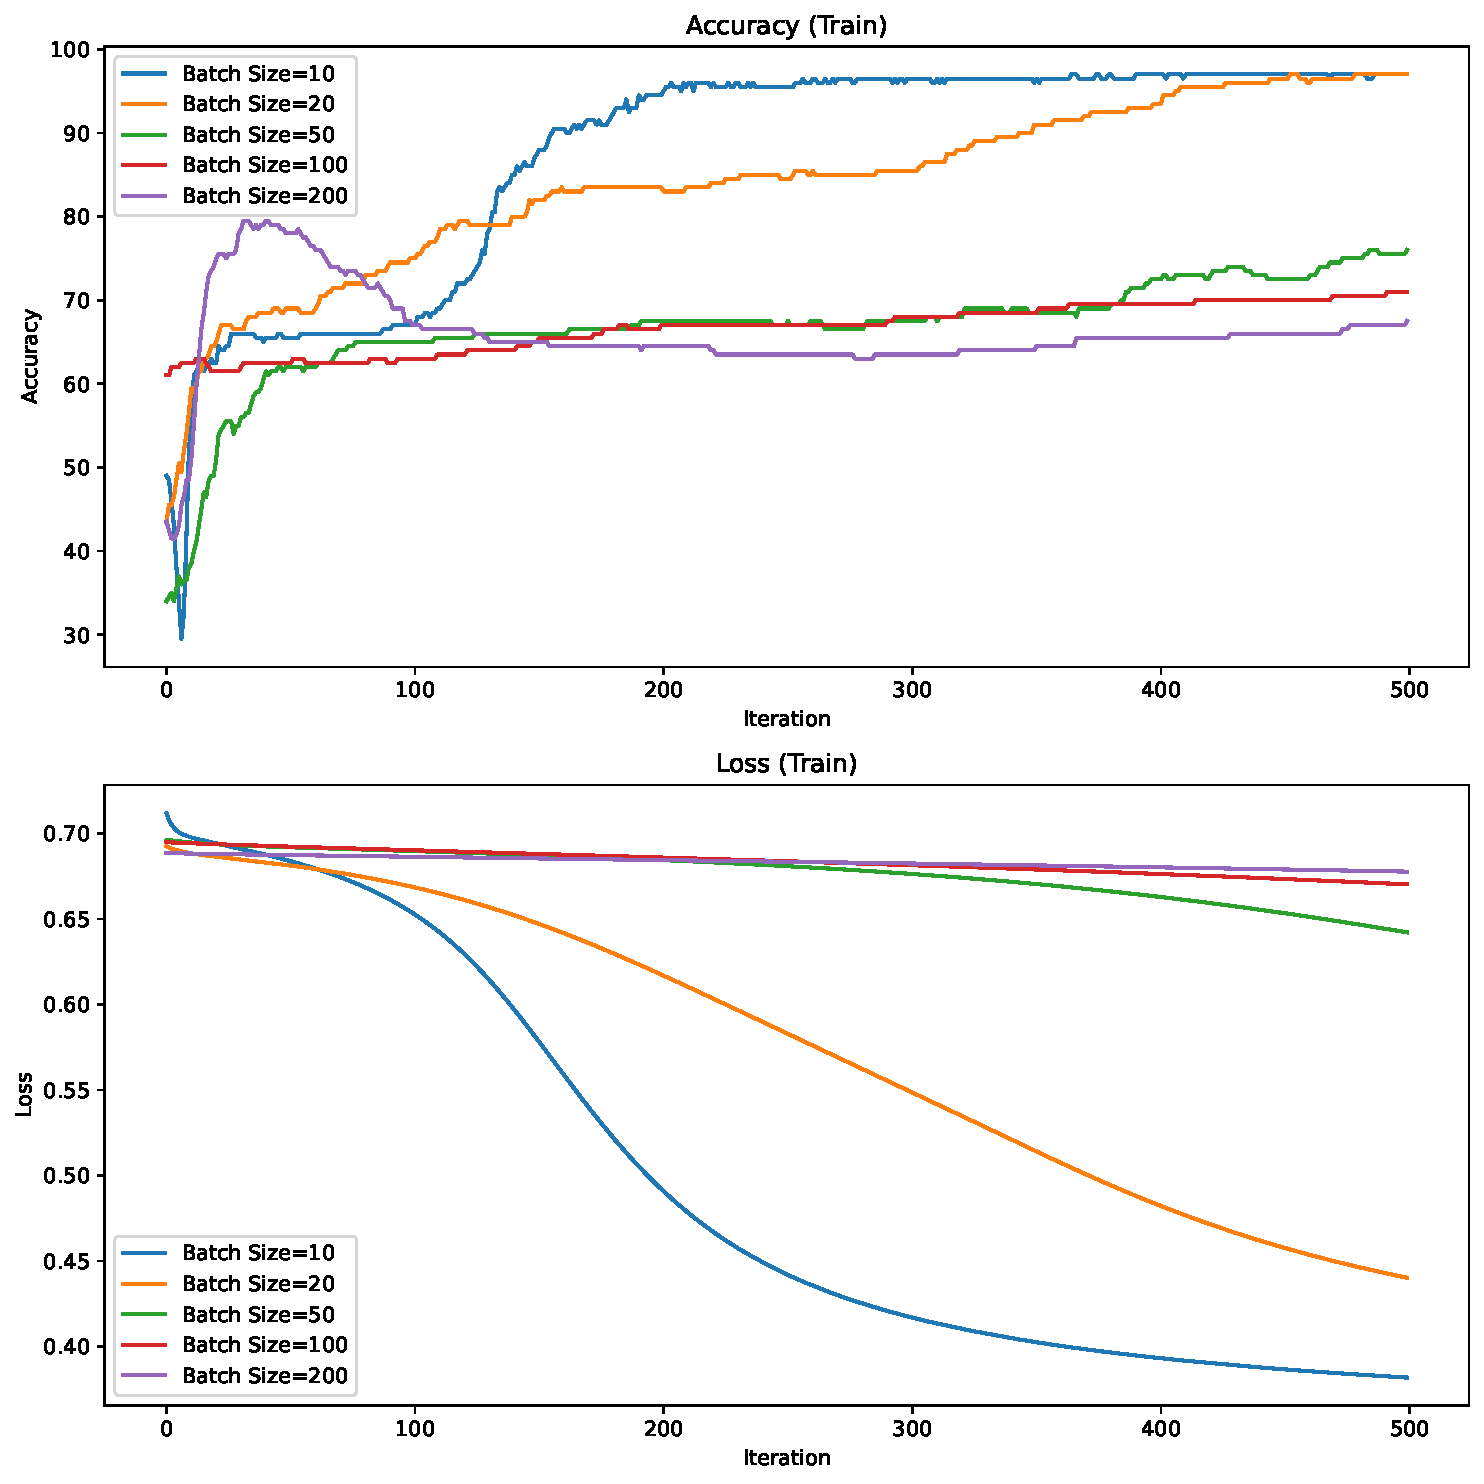
\includegraphics[width=\textwidth]{figs/NN/torchoptim_batchsize.pdf}
        \caption{Influence of batch size}
        \label{subfig:torchoptim_batchsize}
    \end{subfigure}
    \begin{subfigure}{0.45\textwidth}
        \centering
        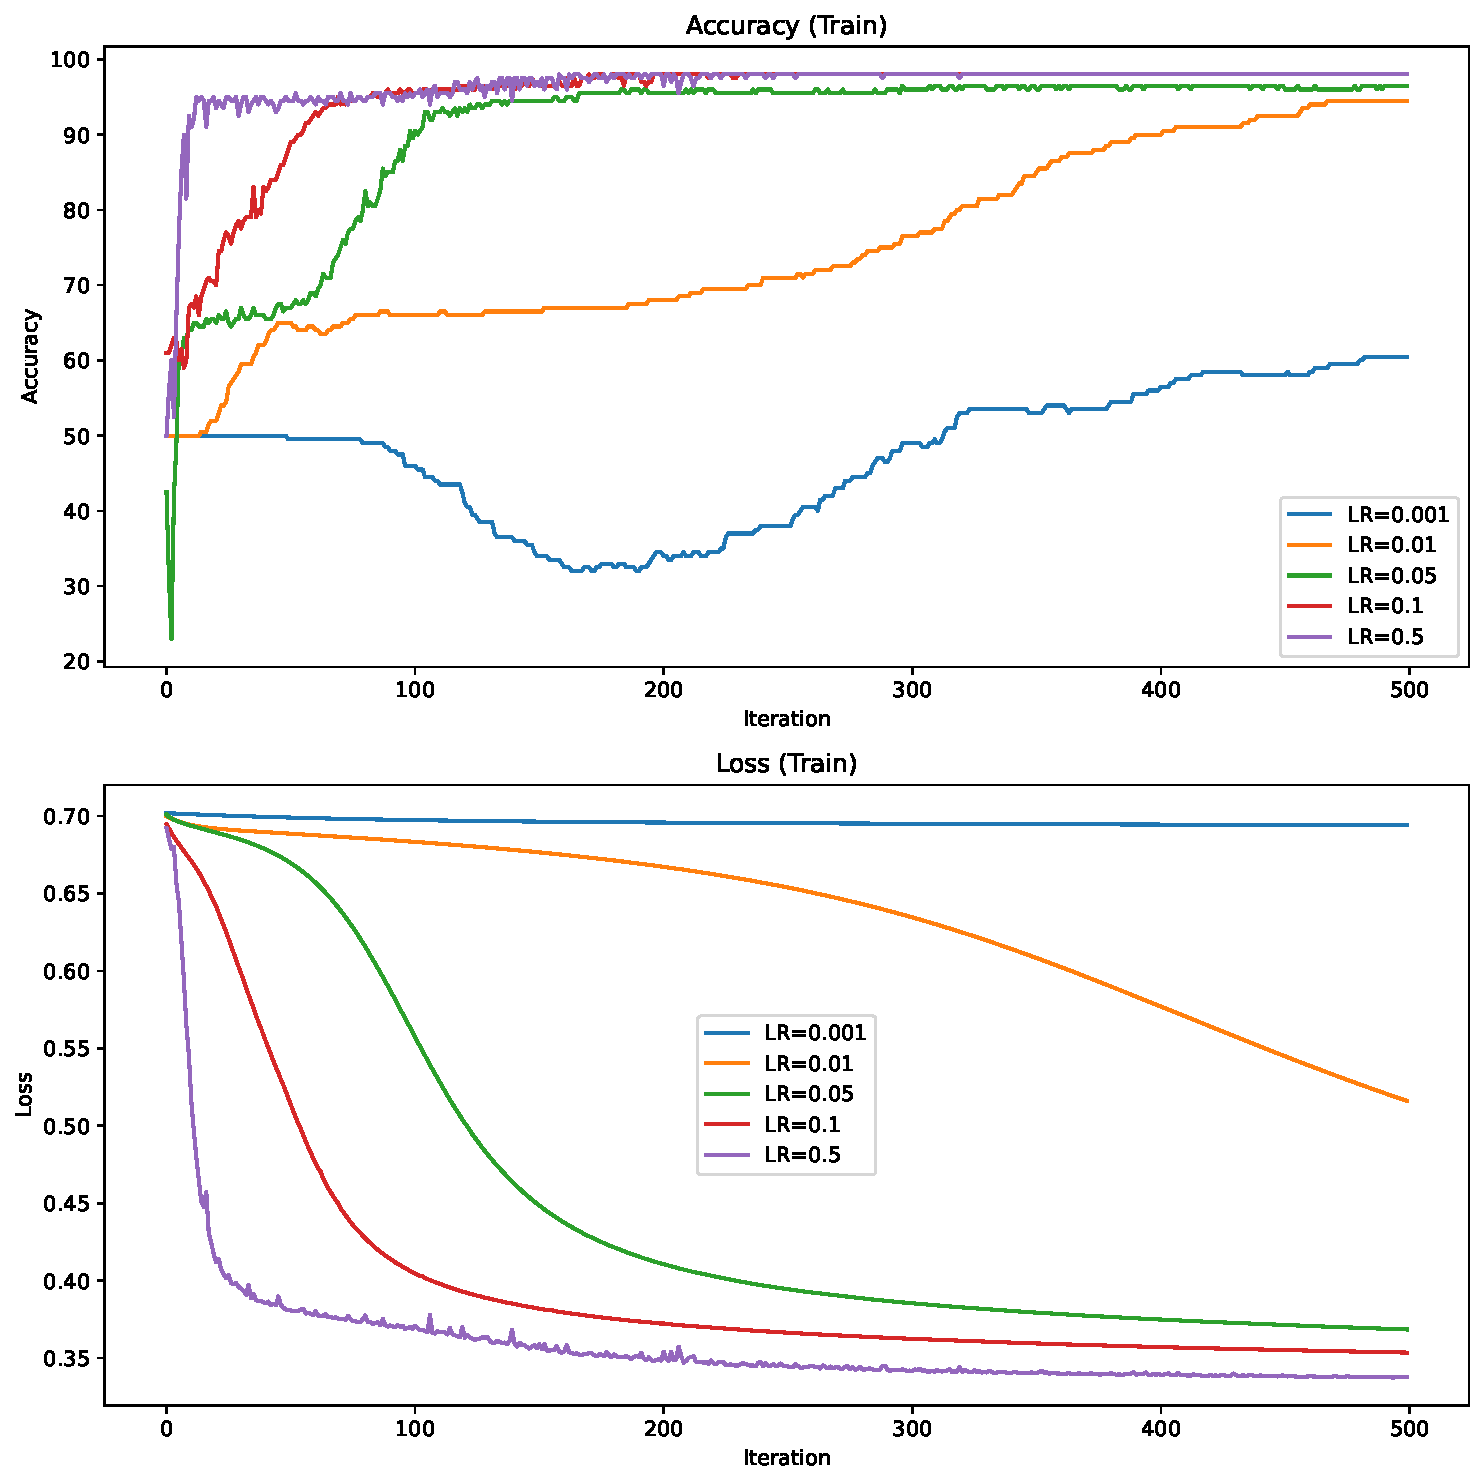
\includegraphics[width=\textwidth]{figs/NN/torchoptim_lr.pdf}
        \caption{Influence of learning rate}
        \label{subfig:torchoptim_lr}
    \end{subfigure}
    \caption{\texttt{torch.optin} }
    \label{fig:torchoptim}
\end{figure}

\subsection{MNIST application}
The following section presents the results of our model on the MNIST dataset, as shown in \Cref{fig:mnist}. Despite its simplicity, the model performs remarkably well. However, there is some instability, which can likely be addressed with a learning rate scheduler or by trying a different optimizer.

\begin{figure}[H]
    \centering
    \begin{subfigure}{\textwidth}
        \centering
        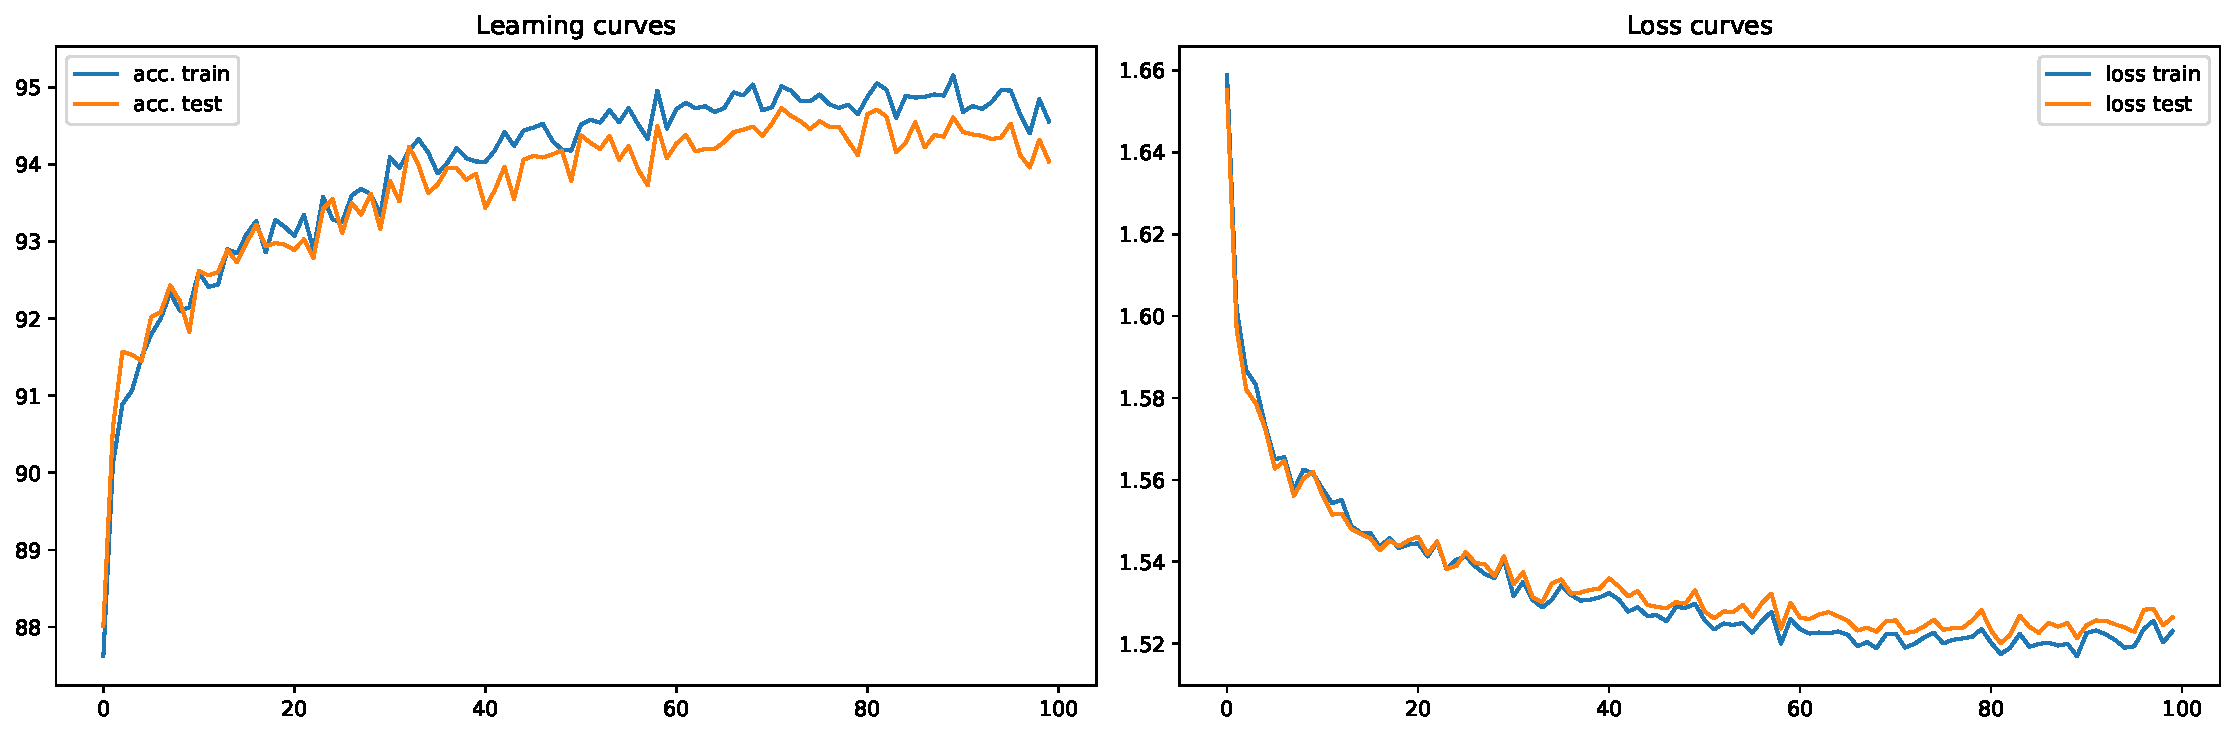
\includegraphics[width=0.88\textwidth]{figs/NN/mnist_acc_loss.pdf}
        \caption{Accuracy and losses curves of our model on MNIST}
        \label{subfig:mnist_acc_loss}
    \end{subfigure}
    \begin{subfigure}{0.45\textwidth}
        \centering
        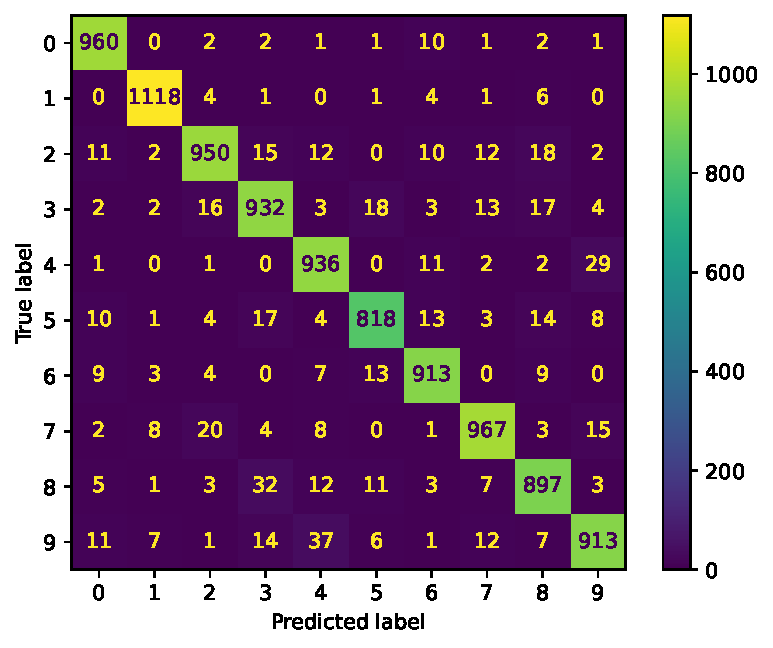
\includegraphics[width=\textwidth]{figs/NN/mnist_cm.pdf}
        \caption{Confusion Matrix}
        \label{subfig:mnist_cm}
    \end{subfigure}
    \caption{Performance on MNIST}
    \label{fig:mnist}
\end{figure}


\subsection{SVM}

We also explored the SVM approach on our circular data, and the decision boundaries, along with their corresponding accuracies, are presented in \Cref{fig:svm_comparison}.

\begin{figure}[H]
    \centering
    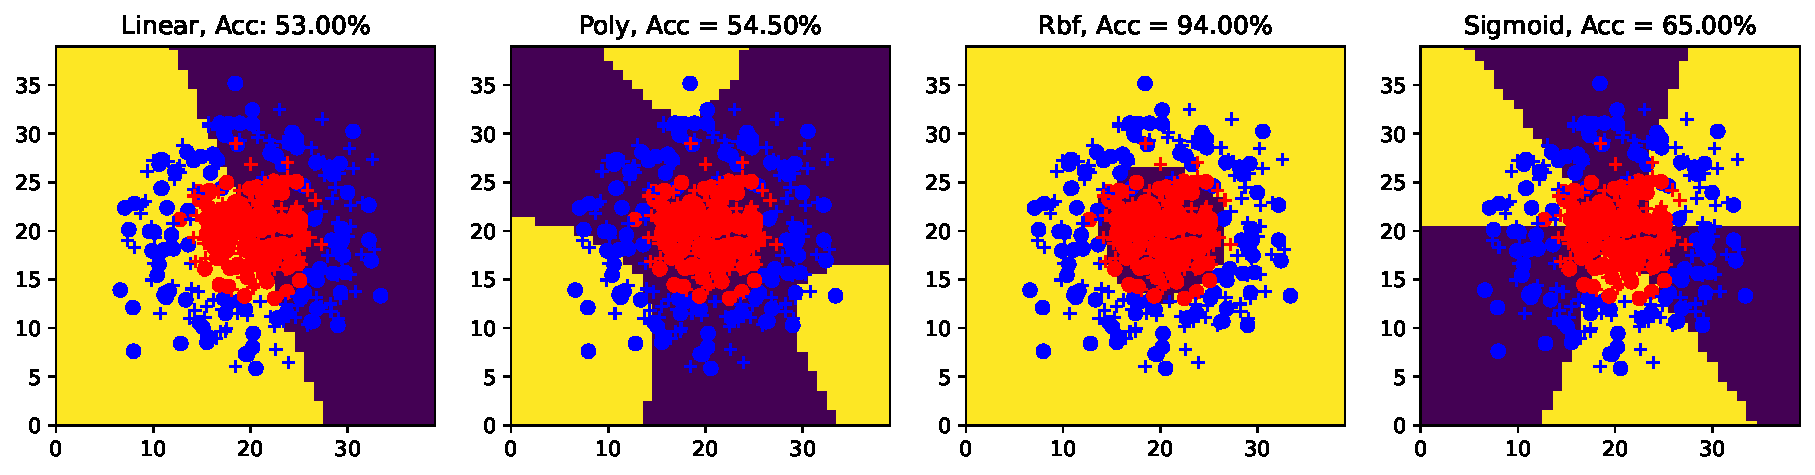
\includegraphics[width=0.9\textwidth]{figs/NN/svm_comparison.pdf}
    \caption{Comparison of SVM}
    \label{fig:svm_comparison}
\end{figure}

It's evident that a linear SVM doesn't work well with circular data. Linear SVMs are designed to find a linear decision boundary that separates data into two classes. Circular data cannot be accurately separated by a single straight line, which is our case here. The Radial Basis Function (RBF) kernel is often the best choice compared to polynomial and sigmoid kernels for circular data because it can capture complex, nonlinear patterns more effectively, and it is better suited to model the circular decision boundaries typically found in such data. RBF kernels can flexibly adapt to various shapes and are more versatile in representing circular patterns, as shown here. It's worth noting that the linear and polynomial kernels did not perform significantly better than a random function.

Furthermore, we conducted experimentations into the influence of the regularization parameter $C$ in the SVM. The results are visualized in \Cref{fig:svm_regularization}. The parameter $C$ in SVMs controls the trade-off between maximizing the margin and minimizing the classification error on the training data.

\begin{itemize}
    \item When $C$ is large, the SVM aims to minimize the classification error on the training data, which results in a smaller margin, meaning that the decision boundary can be more flexible and may even fit noisy data points. This can lead to overfitting. This effect can especially be seen on the polynomial SVM. 
    \item When $C$ is small, the SVM prioritizes maximizing the margin, even if it means allowing some training points to be misclassified. It results in a larger margin, which often leads to a simpler decision boundary. It encourages the SVM to find a more robust decision boundary that generalizes better to unseen data.
\end{itemize}

\begin{figure}[H]
    \centering
    \begin{subfigure}{\textwidth}
        \centering
        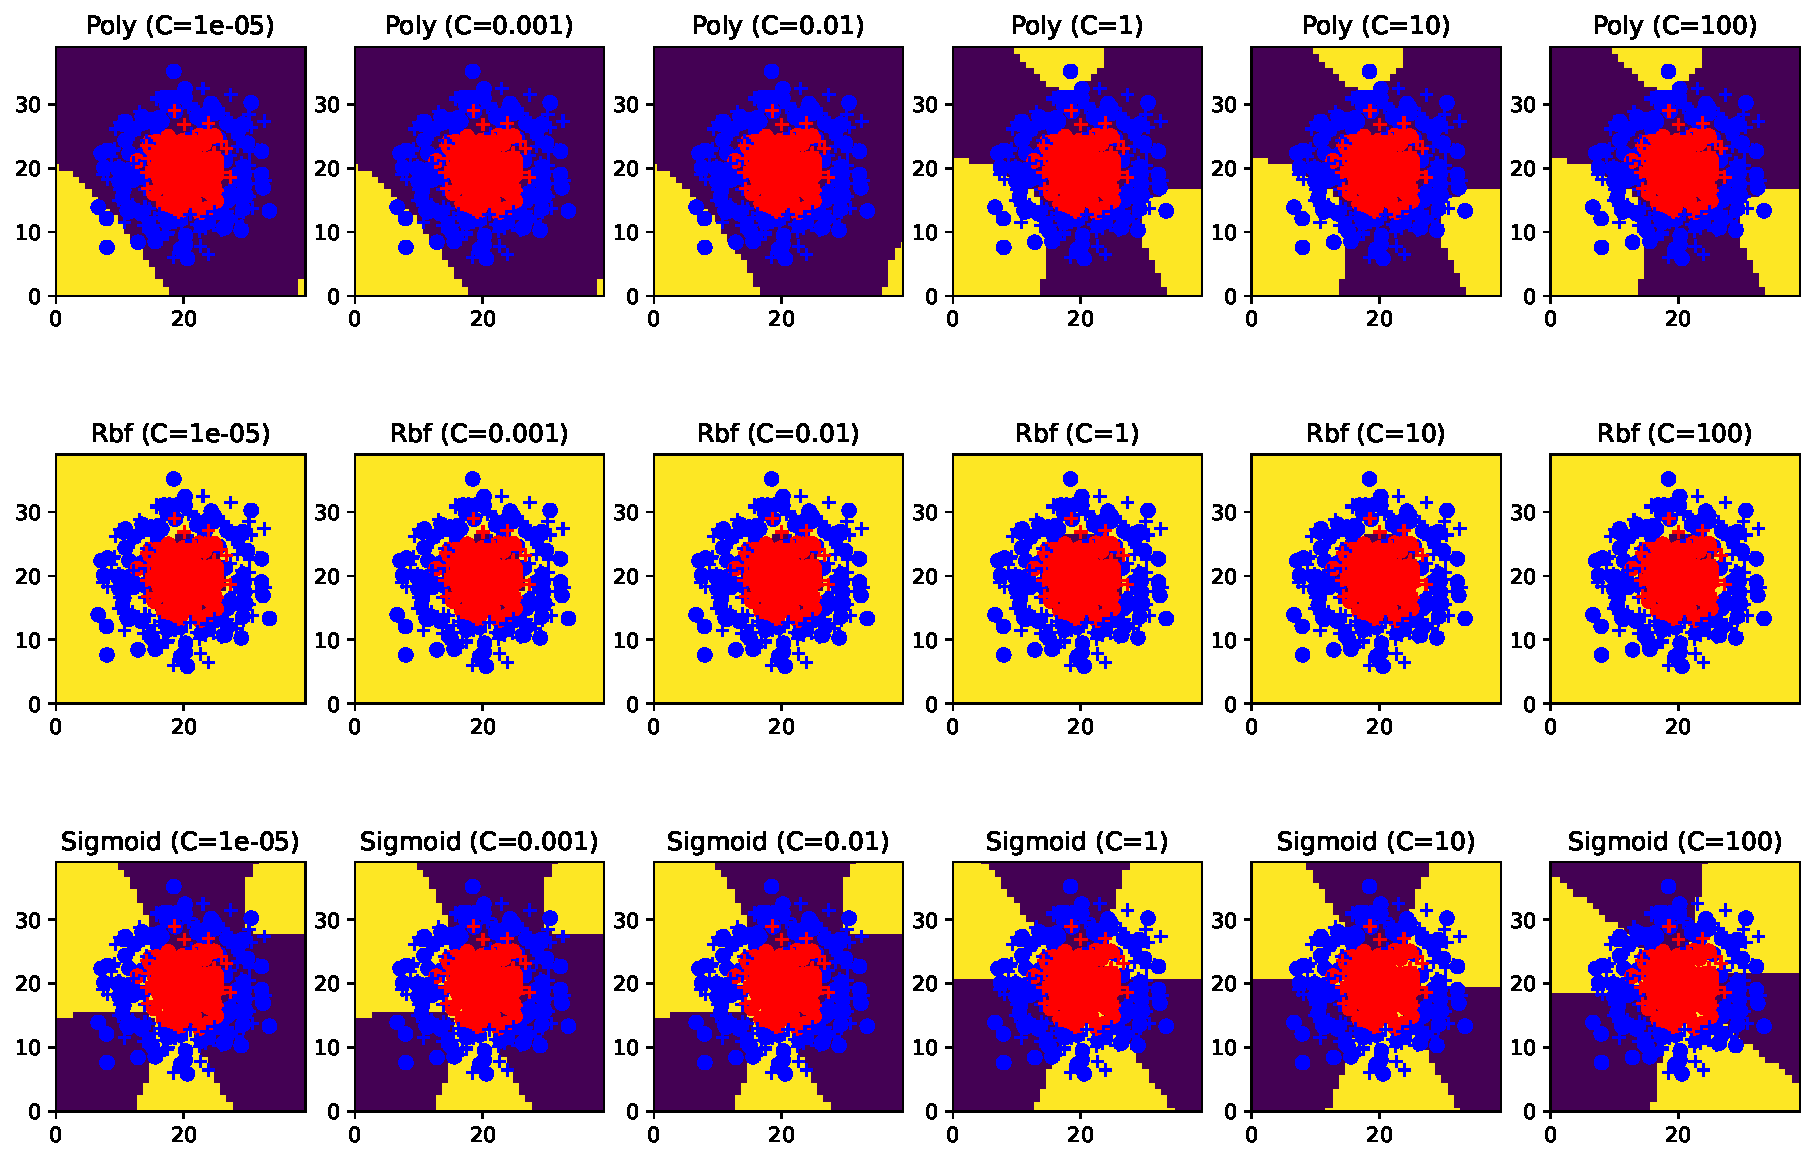
\includegraphics[width=0.9\textwidth]{figs/NN/svm_regularization_grid.pdf}
        \caption{Decision boundaries}
        \label{subfig:svm_regularization_grid}
    \end{subfigure}
\end{figure}

\begin{figure}[H]\ContinuedFloat
    \centering
    \begin{subfigure}{0.9\textwidth}
        \centering
        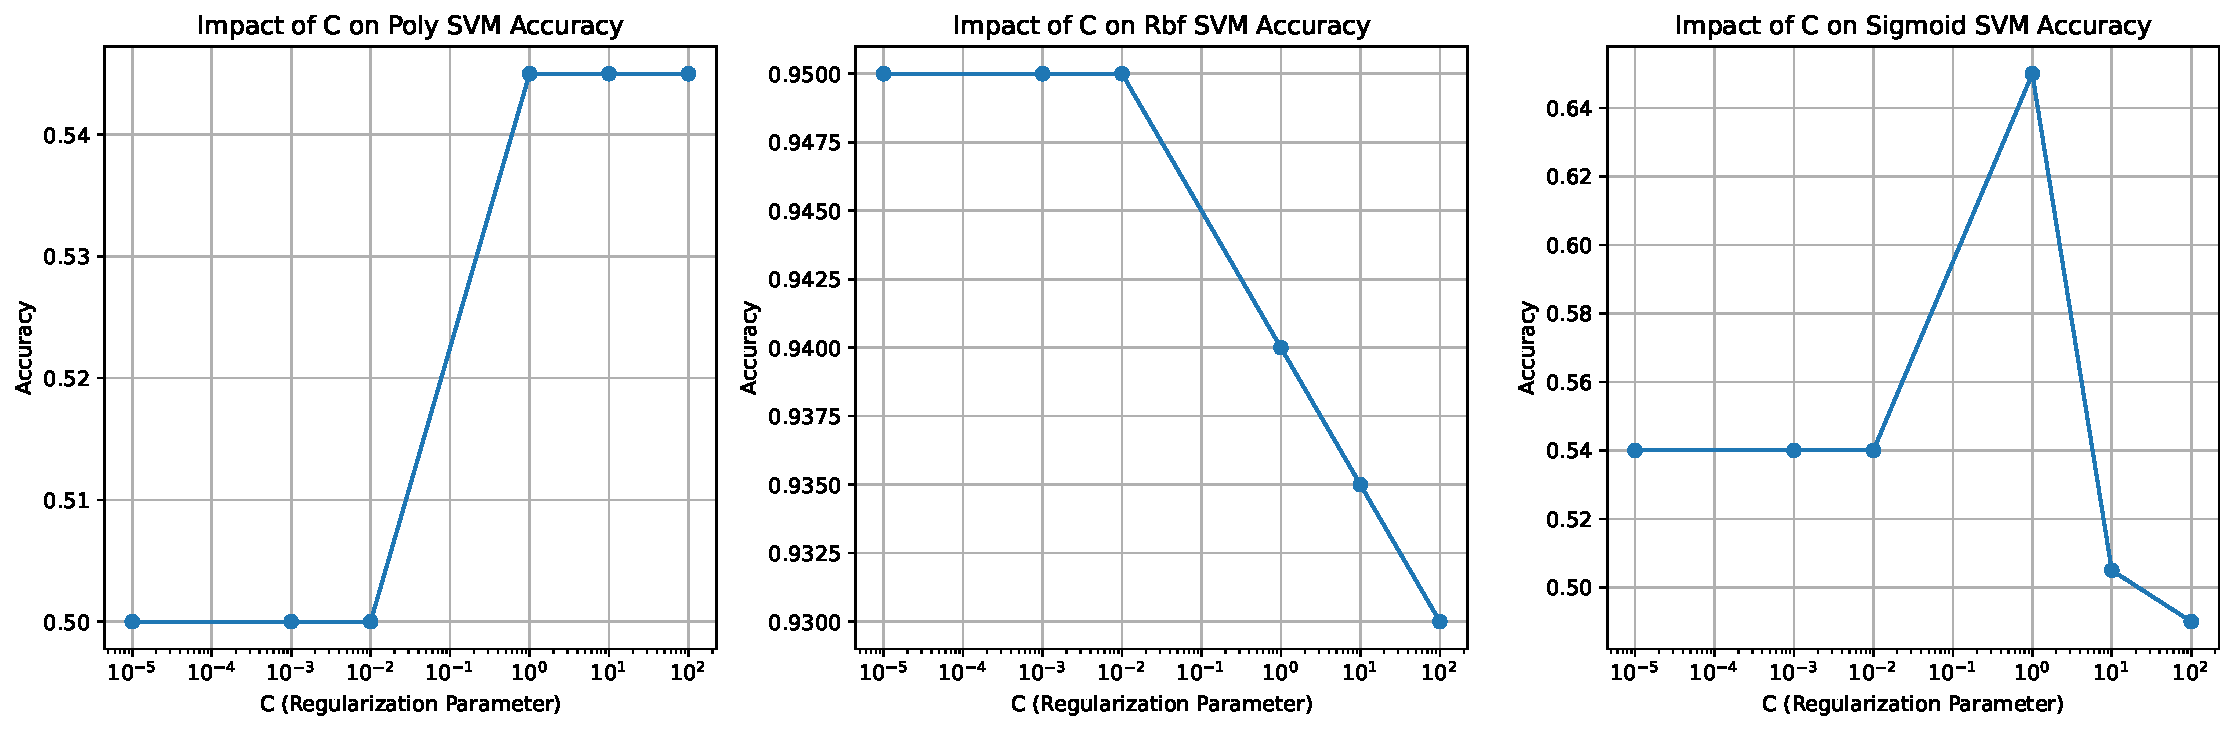
\includegraphics[width=\textwidth]{figs/NN/svm_regularization_acc.pdf}
        \caption{Impact of $C$ on accuracy}
        \label{subfig:svm_regularization_acc}
    \end{subfigure}
    \caption{Influence of regularization parameter}
    \label{fig:svm_regularization}
\end{figure}

\chapter{Introduction to convolutional networks}
\section{Questions}
\paragraph{1. Considering a single convolution filter of padding $p$, stride $s$ and kernel size $k$, for an input of size $x \times y \times z$ what will be the output size? How much weight is there to learn? How much weight would it have taken to learn if a fully-connected layer were to produce an output of the same size?}
Let's note $x_{\text{out}}, y_{\text{out}}, z_{\text{out}}$ our output size. Then, given a convolution filter of padding $p$, stride $s$ and kernel size $k$:

\begin{align}
    \label{eq:1} x_{\text{out}} = \left\lfloor\frac{x - k + 2p}{s} + 1 \right\rfloor \\
    \label{eq:2} y_{\text{out}} = \left\lfloor\frac{y - k + 2p}{s} + 1 \right\rfloor \\
    \label{eq:3} z_{\text{out}} = \text{number of filters} = 1
\end{align}

Given our single convolution filter and our kernel of size $ k \times k $, we thus have $ ((z \times k \times k) + 1) \times z_{\text{out}} = ((z \times k \times k) + 1) $ weights to learn (where "$+1$" represents the bias).

If a fully connected layer were to produce an output with dimensions equivalent to the output of the convolutional layer, it would need to connect every input neuron to every output neuron. For the input layer, every input pixel is a neuron, so there are \(x \times y \times z\) neurons. The total number of neurons in the output layer is \( x_{\text{out}} \times y_{\text{out}} \times z_{\text{out}} \). Thus, considering a bias, there is \((x \times y \times z + 1) \times (x_{\text{out}} \times y_{\text{out}} \times z_{\text{out}}) = (x \times y \times z + 1) \times (x_{\text{out}} \times y_{\text{out}}) \) parameters to learn.

\paragraph{2. $ \bigstar $ What are the advantages of convolution over fully-connected layers? What is its main limit?}
Using fully-connected layers with images involves a substantial number of parameters, one for each pixel of the image. Fully-connected layers are also sensitive to variations in images, including simple translations.

On the other hand, convolutional layers address these issues. By utilizing convolution with a shared set of weights (for filters/kernels) across the entire input, they enable the learning and detection of local spatial patterns and features at various locations. Convolutional layers also possess the ability to hierarchically combine features. Lower layers capture low-level features such as edges and textures, while higher layers capture more intricate features and representations of objects.

However, convolutional layers have limitations in terms of global context. They primarily focus on local patterns and may struggle to comprehend relationships between distant parts of the input, which can be crucial in certain applications (medical imaging, autonomous vehicles...).

\paragraph{3. $ \bigstar $ Why do we use spatial pooling?}
Spatial pooling allows for increased invariance, particularly in the context of translation. By summarizing a local region with a pooled value, the precise feature location becomes less critical. This constitutes a form of regularization that prioritizes the most pertinent information.

Pooling also facilitates dimensionality reduction by decreasing the spatial dimensions of the resulting feature map. This reduction in dimensionality significantly lowers the computational cost of subsequent layers.

Max and average pooling layers are the most commonly employed pooling techniques. Max pooling aids in achieving translation invariance and reducing spatial dimensions. It effectively preserves the most essential features in the input data. On the other hand, average pooling also reduces spatial dimensions and contributes to achieving translation invariance. It can exhibit greater robustness to outliers in the input data when compared to max pooling.

\paragraph{4. $ \bigstar $ Suppose we try to compute the output of a classical convolutional network for an input image larger than the initially planned size. Can we (without modifying the image) use all or part of the layers of the network on this image?}
% By definition, a convolution layer does not dependent of the size of the input, it will take the image, do convolution on it till the end of the image, and output another image. So when staking convolution and pooling layer (which do a convolution too), the output size is only dependent from the input size. In some other words, the input size of the image is not a hyperparameter of the convolution layer.

% In a classical convolutional network, this output from the stacking of convolutionnal and pooling layers is flattened to become the input of a fully-connected layer. The size of the flattened vector is dependent of the size of the outputed image from the convolution layers.

% But this time, we need to know the size of the input of our fully-connected layer in advance to set it up (like to initialse the parameters, ...).

% So when using an input image larger than the initially planned size, everything will run until the use of a fully connected layer because it expect a fixed size input. 
A convolution layer in a convolutional network is size-agnostic regarding its input: it simply performs convolutions across the entire span of the input image and outputs a correspondingly altered image. Sequentially, when convolution and pooling layers are stacked together, the resulting output size is purely a function of the input size. To rephrase, the input size of the image is not a critical hyperparameter for the convolution layer.

Within the conventional architecture of a convolutional network, the output derived from successive convolutional and pooling layers is typically ''flattened'' to form the input for a subsequent fully-connected layer. The size of this flattened vector is contingent on the size of the image output from the preceding convolution layers.

The challenge arises when we involve fully connected layers, as their initialization requires a priori knowledge of their input size to properly set up parameters such as weights. Consequently, when an input image is larger than initially planned, the network can operate normally up to the point of the fully connected layers, which anticipate input of a predetermined, fixed size.

\paragraph{5. Show that we can analyze fully-connected layers as particular convolutions.}
In a fully-connected layer, each pixel of the flattened image is associated with one weight. Both the weights and the flattened image are vectors. However, if we rearrange the weights into a matrix that matches the shape of the image, we can perform element-wise multiplication between this matrix and the image, which is akin to a one slide convolution!

This $1 \times 1$ convolution employs a stride equal to the width of the input image, ensuring that the filter remains fixed and does not slide to different positions. Furthermore, the filter size is exactly the same as the image. The number of filters used in this convolution is equivalent to the number of neurons in the fully-connected layer.

\paragraph{6. Suppose that we therefore replace fully-connected by their equivalent in convolutions, answer again the question 4. If we can calculate the output, what is its shape and interest?}
Fully connected layers usually expect inputs of a specific size. However, if we replace the fully connected layers in a neural network with their convolutional equivalents, we can indeed process images of sizes different from what the network was initially trained on \textit{until the next step} which is the loss computation. 

If an input image larger than the expected size is used, the convolution operations will produce larger feature maps in the intermediate layers, and these will propagate through the network. The final convolutional layers, which replace the fully connected layers, will apply their filters to the full spatial extent of the incoming feature maps. The output shape, in this case, won't be the typical single row of class scores. Instead, it will be a spatial map of scores of size $ (r + 1) \times (c+1) $ where $ r $ is the number of rows added and $ c $ is the number of columns. In this case, this last convolution layer does not act perfectly as a fully connected layers because we still have to know the input size to fix the filter size and the stride ahead.

An issue that arises after the model has undergone the forward pass is computing the loss on the spatial map of scores, as typical loss functions expect a single row of class scores. One potential solution is to employ Average Pooling on the spatial map of scores, aggregating the scores spatially to obtain a single row of class scores suitable for loss computation.

\paragraph{7. We call the receptive field of a neuron the set of pixels of the image on which the output of this neuron depends. What are the sizes of the receptive fields of the neurons of the first and second convolutional layers? Can you imagine what happens to the deeper layers? How to interpret it?}
% Calculating the receptive field's size is done based on the kernel size, stride, and padding of the convolutional layers, and it grows progressively larger in deeper layers due to successive convolutions.

The receptive field $l_k$ of layer $k$ is:

\[ l_k = l_{k-1} + \left((f_k - 1) \times \prod_{i=1}^{k-1}s_i\right) \]

where $l_{k-1}$ is the receptive field of layer $k-1$, $f_k$ is the filter size (height or width, but assuming they are the same here), and $s_i$ is the stride of layer $i$.

The formula above calculates receptive field from bottom up (from layer 1). Intuitively, a receptive field in layer $k$ covers $(f_k - 1) \times s_{k-1}$ more pixels relative with layer $k-1$. However, the increment needs to be translated to the first layer, so the increments is a factorial: a stride in layer $k-1$ is exponentially more strides in the lower layers. In our case, the receptive field of the first convolutional layer is of size 5, which matches the size of the kernel. Consequently, the size of the receptive field of the second layer increases to $ 5 + (5 - 1) = 9 $. This means that each pixel in the output of the second layer takes into account information from 9 pixels in the previous layer. As the neural network progresses into deeper layers, the receptive field continues to grow. When done correctly, the receptive field size of the final layer will match the size of the input image, allowing each pixel in the output to gather information from every pixel in the input image. One can think of the receptive fields as the "eyes" of the neural network.

% TODO https://distill.pub/2019/computing-receptive-fields/#solving-receptive-field-region 

\section{Training \textit{from scratch} of the model}
\subsection{Network architecture}
\paragraph{8. For convolutions, we want to keep the same spatial dimensions at the output as at the input. What padding and stride values are needed?}
We want $ x = x_{out}$, $ y = y_{out} $: let's use our equations \ref{eq:1}, \ref{eq:2} to find the values of $p$ and $s$.
\[
    p = \frac{(s-1)x + k - s}{2}
\]
Knowing $k = 5$ and that our images are of size $32 \times 32 $, we can pick any $p = \frac{31s - 27}{2}$. Since we typically aim to utilize all available pixels in an image while minimizing the need for padding, we choose a stride value of $ s = 1 $ and a padding value of $ p = 2 $, which minimize both parameters.

\paragraph{9. For max poolings, we want to reduce the spatial dimensions by a factor of 2. What padding and stride values are needed?}
A pooling layer acts like a convolution: let's proceed as in question 8. This time we want $ x_{out} = x/2$, $ y_{out} = y/2 $.
\[
    p = \frac{(\frac{1}{2}s - 1) x + k - s}{2}
\]
Knowing $k = 2$ and that our images are of size $32 \times 32 $, we can pick any $p = \frac{15s - 30}{2}$. Following the same logic as in the previous question, we opt for a stride value of $ s = 2 $ and a padding value of $ p = 0 $, which minimize both parameters.

\paragraph{10. $ \bigstar $ For each layer, indicate the output size and the number of weights to learn. Comment on this repartition.}
To simplify the presentation, we have provided a plot of the CNN architecture in \Cref{fig:AlexNetstylelog}. In this architecture, we begin with a 3-channel image measuring 32 by 32 pixels. As mentioned in questions 8 and 9, convolutional layers maintain the same spatial dimensions in the outputs as in the inputs, while pooling layers reduce the spatial dimensions by a factor of two. The following is a breakdown of the number of parameters:
\begin{itemize}
    \item conv1: 32 filters of 5 by 5 for 3 channels $\rightarrow 32\times 5\times 5\times 3 = 2,400$ parameters (plus one biases per channel if activated)
    \item conv2: 64 filters of 5 by 5 for 32 channels $\rightarrow 64\times 5\times 5\times 32 = 51,200$ parameters (plus one biases per channel if activated)
    \item conv3: 64 filters of 5 by 5 for 64 channels $\rightarrow 64\times 5\times 5\times 64 = 102,400$ parameters (plus one biases per channel if activated)
    \item 1000 neurons with 1024 values as input $\rightarrow (1000 + 1)\times 1024=1,025,024$ parameters. The "$+1$" is for biases.
    \item 10 neurons with 1000 values as input $\rightarrow 11\times 1000=11,000$ parameters
\end{itemize}

The fully connected layer \texttt{fc4} alone accounts for up to 86~\% of the total number of parameters, underscoring the significant computational demands associated with these layers during the learning process.

% \begin{figure}[!htbp]
%     \centering
%     \includegraphics*[width=\textwidth]{figs/AlexNet_style.png}
%     \caption{}
%     \label{AlexNetstyle}
% \end{figure}
\begin{figure}[H]
    \centering
    \includegraphics*[width=\textwidth]{figs/AlexNet_style_log.png}
    \caption{Network architecture}
    \label{fig:AlexNetstylelog}
\end{figure}

\paragraph{11. What is the total number of weights to learn? Compare that to the number of examples.}
This leads to a total of 1,192,024 parameters for training. Considering a dataset comprising 50,000 training samples and 10,000 test samples, totaling 60,000 examples (with 6,000 images per class), it does warrant caution regarding the potential for overfitting.

\paragraph{12. Compare the number of parameters to learn with that of the BoW and SVM approach.}
The complexity and, hence, the number of parameters in a BoW and SVM approach depend on the chosen visual vocabulary size. For instance, employing a dictionary of 1000 visual words for the task of classifying 10 classes would result in \( (1000 + 1) \times 10 = 10,010 \) parameters to be learned. It's important to note that in this approach, we also need to fine-tune the hyperparameters of our classifier, with the kernel type and the regularization parameter \( C \) being the most significant. As a result, the parameter space in this approach is considerably smaller when compared to our deep CNN model.
%% Je crois que c'est ça : dans un SVM le nombre de paramètres à apprendre c'est les poids (+ biais) qui sont définis par l'input, ici un BoW. Vu qu'on a 10 classes, on applique la stratégie du one-vs-all, donc on a 10 SVMs (1 par classe). Le BoW c'est juste une représentation spéciale de l'input (des images) : on calcule des features (SIFT), on cluster (K-Means) et on a nos "visual words" en calculant les histogrammes pour chaque image. Donc le nombre de visual words = nombre de bins de l'histogramme.
%% Si c'est pas clair faut reprendre le TME0...

\subsection{Network learning}
\paragraph{14. $ \bigstar $ In the provided code, what is the major difference between the way to calculate loss and accuracy in train and in test (other than the the difference in data)?}
The difference in the code lies in the fact that we do not provide an optimizer to the \texttt{epoch()} function. Consequently, we do not train the network using test examples, and there is no backward pass to calculate and update the loss.
% Le code de base compute la loss à chaque batch, alors qu'on change les paramètres à chaque batch, donc ça rend les comparaisons plus difficile. En général (et c'est ce que j'ai changé dans le code), on compute la loss

\paragraph{16. $ \bigstar $ What are the effects of the learning rate and of the batch-size?}
The learning rate and batch size are critical hyperparameters that significantly impact training performance, speed, and stability:

\begin{itemize}
    \item A high learning rate can cause the model to overshoot the minimum, causing divergent behavior and an inability for the model to learn effectively. On the other hand, having a low learning rate can slow down the training process significantly, possibly leading to a premature convergence to suboptimal solutions. In some cases, a lower learning rate results in a more precise convergence by allowing the model to explore the parameter space thoroughly. \Cref{fig:learning_rate_influence} illustrates the effects of different learning rates with a fixed batch size of 32.
    \item Larger batch size provides a more accurate estimate of the gradient, potentially leading to more stable and consistent training steps. However, this comes with increased memory usage. Conversely, smaller batch sizes can introduce noise, making the path to convergence less direct and possibly longer in terms of epochs. Smaller batches reduce memory requirements, making them suitable for resource-constrained systems. \Cref{fig:batch_size_influence} illustrates the impact of various batch sizes with a fixed learning rate of 0.01.

\end{itemize}

It's important to note that learning rate and batch size are often interrelated. Changes in batch size may require adjusting the learning rate to maintain training quality. This relationship arises from the need to balance the aggressiveness of updates when averaging gradients across more samples. Typically, a linear scaling rule is applied: multiplying the batch size by a factor $k$ also multiplies the learning rate by $k$, while keeping other hyperparameters constant. This relationship is shown in \Cref{fig:linear_scaling}.

\begin{figure}[H]
    \centering
    \includegraphics*[width=0.9\textwidth]{figs/CNN/learning_rate_influence.pdf}
    \caption{Influence of learning rate with a batch size fixed at 32}
    \label{fig:learning_rate_influence}
\end{figure}

\begin{figure}[H]
    \centering
    \includegraphics*[width=0.9\textwidth]{figs/CNN/batch_size_influence.pdf}
    \caption{Influence of batch size rate with a learnig rate fixed at 0.01}
    \label{fig:batch_size_influence}
\end{figure}

\begin{figure}[H]
    \centering
    \includegraphics*[width=0.9\textwidth]{figs/CNN/linear_scaling.pdf}
    \caption{Relationship between batch size and learning rate}
    \label{fig:linear_scaling}
\end{figure}

\paragraph{17. What is the error at the start of the first epoch, in train and test? How can you interpret this?}

For the following experiments, we will compare our results with those presented in \Cref{fig:base_result}, where a batch size of 128 and a learning rate of 0.01 were employed.

\begin{figure}[H]
    \centering
    \includegraphics*[width=0.9\textwidth]{figs/CNN/base_result.pdf}
    \caption{Accuracy and losses in train and test}
    \label{fig:base_result}
\end{figure}

% At the initial epoch, we observed respective accuracies of 0.0101 on the training set and 0.0989 on the test set, along with corresponding losses of 2.3007 and 2.2976.

The situation where test accuracy surpasses training accuracy at the beginning can be attributed to the fact that training loss and accuracy are calculated at each batch, implying that parameters and, consequently, results (loss and accuracy) fluctuate considerably before the completion of the first epoch. This means that during the first batch of the first epoch, the loss is computed based on only a subset of the data equal to the batch size. In contrast, test loss and accuracy are determined at the end of the first epoch, after the model has been exposed to the entire training dataset. These values are more reliable than those obtained from the training phase at the outset of the first epoch.

% At the first epoch, we have respectively in train and test an accuracy of 0.0101 and of 0.0989 for a loss of 2.3007 and 2.2976. 

% The accuracy on the test set is better that the accuracy on train. It's because.
% We must be aware that the training loss and accuracy is calculated \textbf{at every batch} so before the end of the first epoch, parameters and so result (loss and accuracy) are variating a lot. It mean that at the first batch of the first epoch we take into account the loss calculated only with \textit{batch\_size} examples.

% Contrary to the test loss and accuracy that are computed at the end of the first epoch, after the model have seen all training example. Those value are more true that those from train at the first epoch % pire phrase

\paragraph{18. $ \bigstar $ Interpret the results. What's wrong? What is this phenomenon?}
We observe overfitting, as our caution led us to anticipate. This phenomenon becomes evident around the thirtieth epoch when our test accuracy plateaus at approximately 60~\%, while the training accuracy continues to improve. This signifies that while the model is improving its performance on the training dataset, it is struggling to generalize effectively to new, unseen test images.

\section{Results improvements}
\subsection{Standardization of examples}
\paragraph{19. Describe your experimental results.}

Standardization helps mitigate the issues caused by the varying scales and ranges in raw data. By doing this, we can expect improved model training, consistent data distribution and reduced numerical instability. In our experimental results, we do find that standardizing accelerates model training, as we need 20 less epochs to reach convergence in train. Furthermore, we observe increased stability, both in loss and accuracy.

\begin{figure}[H]
    \centering
    \includegraphics*[width=0.9\textwidth]{figs/CNN/standardization.pdf}
    \caption{Accuracy and losses in train and test using standardization}
    \label{fig:standardization}
\end{figure}

\paragraph{20. Why only calculate the average image on the training examples and normalize the validation examples with the same image?}
This practice guarantees that the model evaluates its performance on data processed similarly to the training data, without any prior knowledge of the validation set's specific characteristics. Calculating these statistics using the validation set would result in "data leakage", where the model gains insights into the validation data. This approach is essential for an impartial evaluation of the model's performance and its ability to generalize to new, unseen data.

\paragraph{21. Bonus: There are other normalization schemes that can be more efficient like ZCA normalization. Try other methods, explain the differences and compare them to the one requested.}

A few common normalization techniques are :

\begin{itemize}
    \item \textbf{Global Contrast Normalization}: this technique involves normalization of images by subtracting the mean of the entire image (not per channel) and dividing by the standard deviation of the entire image. GCN is aimed at reducing the effect of lighting variations by flattening the image illumination and enhancing contrast.
    \item \textbf{PCA/ZCA Whitening}: these are linear algebra techniques that aims to decorrelate features. This is beneficial because decorrelated features can improve the learning efficiency of some models. ZCA is a variant of PCA that maintains the original data representation whereas PCA completely destroys it. However, these techniques can be computationally intensive.
    \item \textbf{L1/L2 Normalization}: this technique normalizes the pixels of the image by dividing each pixel value by the L1 (sum of absolute pixel values) or L2 norm (square root of the sum of the squared pixel values) of the image. This normalization is useful when we want to measure the relative importance of pixel values rather than their absolute magnitudes.
    \item \textbf{Min-Max Scaling}: this technique involves rescaling the range of pixel intensity values. Each pixel value is scaled based on the minimum and maximum pixel values found in the dataset. This is a simple scaling technique but does not handle outliers well.
\end{itemize}

We performed a comparison of these techniques, and the results are displayed in \Cref{fig:standardization_influence}. It is worth noting that PCA proved to be computationally demanding, doubling the required training time. L1 standardization exhibited poor performance, which we suspect may be attributed to the normalization process involving the division of each pixel value by the sum of absolute pixel values, resulting in excessively low values. L2 normalization performed better than its counterpart during training but did not generalize effectively during testing. In contrast, per-channel standardization consistently ranks among the top-performing methods, demonstrating superior performance. It's worth noting that there is little to no discernible difference in performance between per-channel standardization and its global counterpart, GCN.

\begin{figure}[H]
    \centering
    \includegraphics*[width=0.9\textwidth]{figs/CNN/standardization_influence.pdf}
    \caption{Influence of standardization techniques}
    \label{fig:standardization_influence}
\end{figure}

\subsection{Increase in the number of training examples by \textit{data increase}}
\paragraph{22. Describe your experimental results and compare them to previous results.}

By artificially increasing our dataset, we expect to have a model that generalize better, as it becomes less sensitive to the specifities of the training images, due to the introduction of variability. Moreover, random crops and flips introduce a level of perturbation to the data, helping the model to become more robust to variations it might encounter in real-world scenarios.

\begin{figure}[H]
    \centering
    \includegraphics*[width=0.9\textwidth]{figs/CNN/dataincrease.pdf}
    \caption{Accuracy and losses in train and test using data augmentation}
    \label{fig:dataincrease}
\end{figure}

Our experimental results demonstrate that our model exhibits improved generalization and reduced overfitting, which is a positive outcome. However, it's important to note that we still observe some degree of instability in testing.

\paragraph{23. Does this horizontal symmetry approach seems usable on all types of images? In what cases can it be or not be?}
For many general tasks, especially those involving natural scenes or objects, horizontal flipping does not change the essence of the subject. For instance, a car is still recognizable as a car, whether flipped or not. This technique is effective in such contexts, contributing to model robustness without misleading the training process. However, in tasks where orientation is crucial to the object's identity or the scene's context, flipping may not be suitable. For example, in handwritten text recognition, letter and number orientation is fundamental, and flipping changes the characters' semantics. Similarly, in scenarios like medical imaging, where a left-right flip might alter the diagnosis (consider organs' positions), this method is not applicable.

\paragraph{24. What limits do you see in this type of data increase by transformation of the dataset?}
Augmentation can sometimes exacerbate class imbalances, particularly if transformations are applied uniformly across classes without considering their initial distribution. Augmenting already overrepresented classes can intensify the imbalance. Some transformations might introduce features that are unnatural, potentially leading the model to learn false patterns. For instance, excessive rotation or scaling might create unnatural shapes or perspectives that the model might wrongly interpret as relevant features. Data augmentation, especially sophisticated methods, increases the computational burden. It requires additional processing for each image and can slow down the training process, demanding more efficient hardware solutions. While augmentation expands the dataset, it doesn't contribute new information beyond the initial data's constraints. The transformations create variability but within the context of existing data, possibly limiting the model's ability to generalize in radically new scenarios.

\paragraph{25. Bonus: Other data augmentation methods are possible. Find out which ones and test some.}
A wide array of augmentation methods is available, including but not limited to rotation, flips, zooming, perspective alteration, affine transformations, color adjustments (brightness, contrast, saturation, hue), sharpness modification, Gaussian blur, polarization, solarization, pixel erasure, channel permutation, grayscale conversion, and more.

We tried random erasing and random rotation (0° to 180°) on the train dataset and random rotation (0° to 90°) on the test dataset. Results are displayed on \Cref{fig:dataincrease_rotation}.

\begin{figure}[H]
    \centering
    \includegraphics*[width=0.9\textwidth]{figs/CNN/dataincrease_rotation.pdf}
    \caption{Accuracy and losses in train and test using data augmentation}
    \label{fig:dataincrease_rotation}
\end{figure}

One may also wonder what happens when we train a model using certain transformations and test it using transformations that the model hasn't encountered during training. \Cref{fig:dataincrease_bis} illustrates the consequences of this approach, where we applied random erasing and random rotation (0° to 180°) to the training dataset and random rotation (180° to 360°) to the test dataset. This experiment highlights that even though both involve rotations, the model may struggle to generalize when faced with previously unseen transformations.

\begin{figure}[H]
    \centering
    \includegraphics*[width=0.9\textwidth]{figs/CNN/dataincrease_bis.pdf}
    \caption{Accuracy and losses in train and test using data augmentation}
    \label{fig:dataincrease_bis}
\end{figure}

As a final note, we want to mention that as we introduced more transformations, we observed a significant increase in training time, with the training process taking at least twice as long. This highlights the computational complexity associated with this technique, as discussed in question 24.

\subsection{Variants of the optimization algorithm}
\paragraph{26. Describe your experimental results and compare them to previous results, including learning stability.}

Incorporating a learning rate scheduler controls how quickly or slowly a model adapts to the problem at hand. Thus, we expect a controlled model convergence, as the model's training process benefits from a more cautious approach to reaching the global minimum of the loss function by gradually decreasing the learning rate. It should also permits to avoid plateaus, i.e. regions where the model's accuracy does not improve significantly due to slow learning. Last, we expect an enhanced training stability.

\Cref{fig:optim_variants} depicts our results. We can see that the loss curve exhibits greater stability when compared to the baseline results (refer to \Cref{fig:base_result}).

\begin{figure}[H]
    \centering
    \includegraphics*[width=0.9\textwidth]{figs/CNN/optim_variants.pdf}
    \caption{Accuracy and losses using an exponential decay scheduler with SGD}
    \label{fig:optim_variants}
\end{figure}

\paragraph{27. Why does this method improve learning?}
The fundamental reason exponential decay learning rate scheduling improves learning lies in its dynamic adaptation to the training process's needs. In the early phases of training, where the initial parameters are likely far from optimal, a larger learning rate helps cover more ground. However, as training progresses, it becomes more about refinement, requiring smaller updates to fine-tune the model, something achieved by reducing the learning rate.

Moreover, this method acknowledges that the landscape of the loss function is not uniformly shaped. Some areas might be steep (necessitating larger steps for efficiency), while others might be flat or have a complex curvature (where smaller steps are necessary for finding the precise minimum). An exponential decay schedule for the learning rate adapts to these needs inherently, allowing for a more nuanced and, consequently, more effective approach to model training.

However, it's essential to approach the setting of the initial learning rate and decay factor with care, as these hyperparameters can significantly affect the training's effectiveness and efficiency. Too rapid a decay might mean the learning rate reduces too quickly, curtailing the model's capacity to learn, while too slow a decay might keep the learning rate too high, leading to the aforementioned issues of overshooting or oscillating around the minimum.

\paragraph{28. Bonus: Many other variants of SGD exist and many learning rate planning strategies exist. Which ones? Test some of them.}

In this study, we employed various optimizer configurations and learning rate scheduling techniques. Initially, we visualize the learning rate dynamics throughout the training epochs using \Cref{fig:schedulers_comparison}. Subsequently, we analyze the impact of these scheduling methods on both training and testing accuracies, as well as losses, as demonstrated in \Cref{fig:schedulers_influence}.

\begin{figure}[H]
    \centering
    \includegraphics*[width=0.9\textwidth]{figs/CNN/schedulers_comparison.pdf}
    \caption{Learning rates curves}
    \label{fig:schedulers_comparison}
\end{figure}

\begin{figure}[H]
    \centering
    \includegraphics*[width=0.9\textwidth]{figs/CNN/schedulers_influence.pdf}
    \caption{Influence of different schedulers on SGD}
    \label{fig:schedulers_influence}
\end{figure}

Firstly, it's noteworthy that both the Constant and Linear learning rate schedulers exhibit a tendency to increase the learning rate, resulting in detrimental performance after a considerable number of epochs, even though it might have been beneficial at the beginning (otherwise they would not have showed this behavior). Conversely, all the other schedulers converge to a similar learning rate value, with the Polynomial scheduler being the fastest to reach this point, albeit with a relatively modest performance of approximately 80~\% in train and 70~\% in test. The top three performers among the schedulers are Exponential, Step (which exhibit similar behavior), and Cosine. Cosine, owing to the nature of its function, takes the longest to reach its learning rate plateau.

Additionally, it's essential to recognize that there exist alternative optimizers more effective than SGD. We conducted a comparative analysis, the results of which are depicted in \Cref{fig:optimizers_influence}. Among the optimizers, Adagrad demonstrated the highest performance, closely followed by its variant, Adadelta. Conversely, both AdamW and RMSProp exhibited relatively poorer performance and displayed numerical instability during testing, with Adam occupying an intermediate position. It's noteworthy that none of the optimization methods led to overfitting.

\begin{figure}[H]
    \centering
    \includegraphics*[width=0.9\textwidth]{figs/CNN/optimizers_influence.pdf}
    \caption{Influence of different optimizers}
    \label{fig:optimizers_influence}
\end{figure}

\subsection{Regularization of the network by \textit{dropout}}
\paragraph{29. Describe your experimental results and compare them to previous results.}

Integrating a dropout layer in a neural network is a strategic move to combat the risk of overfitting, especially before a fully connected layer that has a substantial number of weights. Thus, we expect reduced overfitting and enhanced network performance. \Cref{fig:dropout} and \Cref{fig:dropout_with_scheduler} depicts two experiments with dropout.

\begin{figure}[H]
    \centering
    \includegraphics*[width=0.9\textwidth]{figs/CNN/dropout.pdf}
    \caption{Accuracy and losses in train and test, using a dropout on \texttt{fc4}}
    \label{fig:dropout}
\end{figure}

\begin{figure}[H]
    \centering
    \includegraphics*[width=0.9\textwidth]{figs/CNN/dropout_with_scheduler.pdf}
    \caption{Accuracy and losses in train and test, using a dropout on \texttt{fc4} and a scheduler}
    \label{fig:dropout_with_scheduler}
\end{figure}

\paragraph{30. What is regularization in general?}
Regularization refers to techniques that constrain a model's learning capacity indirectly or directly to prevent overfitting, which occurs when a model learns the training data too closely and fails to generalize well to unseen data. Regularization methods work by adding a penalty to the loss function or by manipulating the training data or model architecture. The goal is to discourage the learning of overly complex models, as these are more prone to overfitting, by prioritizing simpler, more generalizable models that perform better on unseen data. Common regularization techniques include L1 and L2 regularization, dropout, data augmentation, early stopping, and even architectural choices like choosing simpler models over more complex ones.

\paragraph{31. Research and "discuss" possible interpretations of the effect of dropout on the behavior of a network using it?}
Dropout is a regularization technique where random neurons (along with their connections) are "dropped out" (or temporarily removed) from the network with a certain probability, preventing their activation, during training.

Dropout forces neurons to learn more robust and independent representations by making the presence of other neurons unreliable. Without dropout, neurons can become co-adapted, meaning they rely on the specific output of other neurons. By randomly removing different neurons, dropout disrupts these potentially intricate co-adaptations, ensuring that each neuron contributes individually to the solution.

Dropout can be interpreted as a form of model averaging or ensemble learning. Each training epoch uses a different "thinned" network, and predictions on unseen data are effectively the aggregated output of these numerous networks. This ensemble approach is known to generally improve model robustness and generalization.

Dropout introduces variability into the network, somewhat akin to injecting noise into the hidden units' outputs. This noise can help prevent the network from fitting the training data too precisely, effectively acting as a form of stochastic data augmentation.

\paragraph{32. What is the influence of the hyperparameter of this layer?}
The hyperparameter of this layer is called the "dropout rate" and represents the probability that any given neuron will be temporarily dropped. A very high dropout rate means more neurons are dropped during training. While this might increase regularization (thus potentially reducing overfitting), if the rate is too high, the network might lose too much information, making learning difficult and possibly leading to underfitting. A lower dropout rate maintains more neurons active but might offer insufficient regularization, making the model still prone to overfitting, especially if it's a complex, deep network. Results of this hyperparameter on our architecture are displayed on \Cref{fig:dropout_hyperparameter}. In our specific case, a minimal dropout rate enhances training performance but leads to overfitting. Conversely, employing a high dropout rate significantly mitigates the overfitting issue. Unexpectedly, setting the dropout rate to $p=1$ (meaning \textbf{\textit{all}} layers are dropped) renders our model incapable of learning.

\begin{figure}[H]
    \centering
    \includegraphics*[width=0.9\textwidth]{figs/CNN/dropout_hyperparameter.pdf}
    \caption{Influence of dropout rate $p$}
    \label{fig:dropout_hyperparameter}
\end{figure}

\paragraph{33. What is the difference in behavior of the dropout layer between training and test?}
During training, neurons are randomly deactivated with each batch of data, with the dropout rate determining the fraction of neurons to drop. This random deactivation happens every time a new batch is fed to the model. During test, dropout is disabled and acts as identity function, meaning all neurons are active. This approach is necessary to prevent the random uncertainty introduced by dropout during training from affecting the model's predictions on new data.

\subsection{Use of \textit{batch normalization}}

\paragraph{34. Describe your experimental results and compare them to previous results.}

oui

\begin{figure}[H]
    \centering
    \includegraphics*[width=0.9\textwidth]{figs/CNN/batchnorm.pdf}
    \caption{Accuracy and losses in train and test using batch normalization and a scheduler}
    \label{fig:batchnorm}
\end{figure}

\begin{figure}[H]
    \centering
    \includegraphics*[width=0.9\textwidth]{figs/CNN/batchnorm_with_dropout.pdf}
    \caption{Accuracy and losses in train and test, using batch normalization, a dropout layer and a scheduler}
    \label{fig:batchnorm_with_dropout}
\end{figure}

\subsection{Combination of all methods}
Now that we have individually explored various methods to enhance our results within a relatively straightforward convolutional network architecture, one might wonder what happens when we combine all these techniques (standardization, data increase, optimizer, scheduler, dropout, batch normalization), much like the Power Rangers assembling with their mechs. Our expectation is that this comprehensive approach will yield significantly improved results characterized by minimal overfitting, strong generalization, and enhanced robustness. Results confirm our expectation and are displayed in \Cref{fig:combined}. It's worth noting that this approach may appear excessive, as it produces results similar to the one obtained using a dropout and a learning rate scheduler.

\begin{figure}[H]
    \centering
    \includegraphics*[width=0.9\textwidth]{figs/CNN/combined.pdf}
    \caption{Accuracy and losses in train and test using all methods}
    \label{fig:combined}
\end{figure}

\chapter{Introduction to transformers}

\begin{figure}[H]
    \centering
    \includegraphics*[width=.8\textwidth]{figs/Transformers/The-Vision-Transformer-architecture-a-the-main-architecture-of-the-model-b-the.png}
\end{figure}

% mettre la source non ?

\section{Self-Attention}
\paragraph{What is the main feature of self-attention, especially compared to its convolutional counterpart? What is its main challenge in terms of computation/memory?}\label{paragraph:complexity}
Unlike convolutional layers that consider a local neighborhood around each input position, self-attention can weigh all positions across the entire sequence (here the image), providing a form of global receptive field. This is beneficial for tasks where the relevant context can be far from the current position. Convolutional layers have a fixed receptive field, which limits their ability to capture long-range dependencies unless many layers are stacked or dilated convolutions are used.

The primary challenge of self-attention is its computational and memory complexity, particularly the quadratic complexity with respect to the sequence length. In self-attention, every element in the input sequence interacts with every other element, leading to a time and space complexity of something like $ O(n^2) $, where $n$ is the length of the input sequence. This makes self-attention computationally expensive and memory-intensive for long sequences.

\paragraph{At first, we are going to only consider the simple case of one head. Write the equations and complete the following code. And don't forget a final linear projection at the end!}

First we need to compute three different linear projection of the input $ X $ : the Query $ Q $, the Key $ K $, and the Value $ V $.

\begin{align*}
    Q & = X W_q, \\
    K & = X W_k, \\
    V & = X W_v
\end{align*}

The main part of attention is the dot product between the Query and the Key. Those are a set of vector that we learn. The goal is to learn representation of Key that answer the Query to orient the attention. The dot product is high where the model need attention.

But we must be aware that when values of the key and query vectors are large, the dot products can become very large. This can result in large values in the softmax function, leading to vanishing gradients during backpropagation. Scaling down the dot products by $ \sqrt[]{d_k} $ (where $ d_k $  is the dimensionality of the query and key vectors) helps in keeping the gradients in a manageable range, which in turn stabilizes the training. As the variance of the dot product grows with the dimensionality, it also keep it constant.

\[
    \text{Attention}(Q, K, V) = \text{Softmax}\left(\frac{QK^t}{\sqrt{d_k}}\right)V
.\]

The Value matrix represents the actual content of the input tokens. Once the attention scores are computed, they are used to weight the value vectors $ V $.

Optionnaly, it's possible to do a last final linear projection at the then, in this case we have 
\[
    \text{Attention}(Q, K, V) = \text{Softmax}\left(\frac{QK^t}{\sqrt{d_k}}\right)V W
.\]


\section{Multi-head self-attention}

\paragraph{Write the equations of Multi-Heads Self-Attention.}
\[
    \text{MultiHead}(Q, K, V) = \text{Concat}(\text{head}_1, ..., \text{head}_h)W^O
    .\]
where $\text{head}_i = \text{Attention}(QW_i^Q, KW_i^K, VW_i^V)$. The Attention function is the same as described in the single-head attention, and $W^O$ is a final linear layer's weights.

\section{Transfomer block}

\paragraph{Write the equations of the transformer block.}
Let's define the operations within a Transformers block:

\begin{enumerate}
    \item Let \( x \) be the input to the Transformers block, which in our case is a patch from the image plus a positional embedding. We begin by normalizing the input using Layer Normalization (LayerNorm):

        \[
            z = \text{LayerNorm}(x)
        \]

    \item We then compute the Query (Q), Key (K), and Value (V) matrices, which are used in the Multi-Head Attention mechanism as explained in the previous question:

        \[
            Q = z \cdot W_q, \quad K = z \cdot W_k, \quad V = z \cdot W_v
        \]

    \item Next, we pass these matrices \( Q \), \( K \), and \( V \) into the Multi-Head Attention mechanism:

        \[
            \text{AttOutput} = \text{MultiHead}(Q, K, V)
        \]

    \item We add the normalized input \( z \) to the output of the Multi-Head Attention and apply Layer Normalization again:

        \[
            \text{MidLayerOutput} = \text{LayerNorm}(z + \text{AttOutput})
        \]

    \item The MLP (Multi-Layer Perceptron) head is a two-layer linear network with a GeLU (Gaussian Error Linear Unit) or ReLU (Rectified Linear Unit) activation function, defined as follows:

        \[
            \text{MLP}(x) = \text{ReLU}(x \cdot W_1 + b_1) \cdot W_2 + b_2
        \]

    Finally, we compute the output of the MLP and add it to the \text{MidLayerOutput} to obtain the final output of the Transformers block:

        \[
            \text{MLPOutput} = \text{MLP}(\text{MidLayerOutput})
        \]
        \[
            \text{FinalOutput} = \text{MLPOutput} + \text{MidLayerOutput}
        \]

    After this last addition, we obtain the final output of a Transformers block.
\end{enumerate}

\section{Full ViT model : Questions}

\paragraph{Explain what is a Class token and why we use it?}
The class token is positionned as the first token. It is represented as a learnable vector which gets updated during the forward pass. It accumulate information from different parts of the image as it gets updated through the Transformer layers. As it sum-up all the image, we use it to classify the image.

\paragraph{Explain what is the positional embedding (PE) and why it is important?}
The PE are used to provide the spacial information to the model. Here we use sinusoidal encoding, it provide a fixed, unique and easy to generate encodding for the position. \Cref{fig:pe_viz} is employed to visualize the appearance of sinusoidal encoding. In the context of an image transformer, the x-axis represents the number of image patches created, while the y-axis represents the size of an image patch embedding.  \\
Another approach is to learn this positional embedding. This method allows the model to learn the most useful positional representations. \\
This positionnal embedding is then sum to the image embedding.

\begin{figure}[H]
    \centering
    \includegraphics*[width=.75\textwidth]{figs/Transformers/positional_encoding_subplot.pdf}
    \caption{Visualization of Sinusoidal Positional Encodings in Transformer Models}
    \label{fig:pe_viz}
\end{figure}

\section{Experiment on MNIST! : Hyperparameters influences}
The overall performance of our small transformer is really good on MNIST. The convergence is quick and the accuracy really high for every experiments.

As we did in previus experiments, we'll analyse the influence of hyperparmeter by ploting loss and accuracy on the train and test dataset.

\subsection{Embed dimension}
First, let's examine the performance of different embedding dimensions in \Cref{fig:embed_dim_influence}. Several notable observations can be made:

In this figure, it's evident that an embedding dimension of 16 takes slightly more epochs to converge compared to other sizes. Conversely, the size of 128 converges at the same speed but achieves the lowest final accuracy and loss. Importantly, this larger size does not exhibit signs of overfitting. It's worth mentioning that training with an embedding size of 128 also requires more time (in terms of minutes) due to the increased number of parameters.

On the other hand, the embedding size of 16 achieves similar performance to the other sizes but with fewer parameters, resulting in reduced energy consumption and training time. This aligns with the principle of Occam's razor, emphasizing the value of simplicity.

\begin{figure}[H]
    \centering
    \includegraphics*[width=0.9\textwidth]{figs/Transformers/embed_dim_influence_25.pdf}
    \caption{Influence of the size of the embed dimension}
    \label{fig:embed_dim_influence}
\end{figure}

\subsection{Patch size}
\Cref{fig:patch_size_influence} illustrates the impact of patch size on the learning process. Similar to the previous paragraph, it's apparent that all conditions ultimately converge to nearly the same level of accuracy. However, the test loss provides more informative insights.

As anticipated, a patch size as small as 2 by 2 pixels encountered greater challenges in learning due to its diminutive dimensions. On the other hand, a patch size of 28 by 28 pixels is equivalent to the size of an MNIST image, and thus, no patches are formed. This particular configuration, along with a patch size of 14 pixels, exhibits the lowest initial loss and maintains this characteristic throughout most of the training epochs.

\begin{figure}[H]
    \centering
    \includegraphics*[width=0.9\textwidth]{figs/Transformers/patch_size_influence_25.pdf}
    \caption{Influence of the patch size}
    \label{fig:patch_size_influence}
\end{figure}

\subsection{Number of transformers blocks}
The influence of the number of transformer blocks is evident in \Cref{fig:nb_block_influence}. This experiment exhibits similarities to the one conducted with embedding sizes. In all configurations, convergence to a high level of accuracy is observed. However, it's important to note that a high number of blocks can potentially result instability in learning, as indicated by the test loss curve when using 8 blocks. This condition also converge to a lower accuracy.

\begin{figure}[H]
    \centering
    \includegraphics*[width=0.9\textwidth]{figs/Transformers/nb_block_influence_25.pdf}
    \caption{Influence of the number of transformers blocks}
    \label{fig:nb_block_influence}
\end{figure}

\subsection{Number of heads in a block}
Plot in \Cref{fig:num_heads_influence} suggests that an increase in the number of self-attention heads tends to yield better results as we can see by looking at accuracy in train and test.
% Additionally, it's noteworthy that the test loss curves do not overlap, which enhances our confidence in the reliability of these results.

\begin{figure}[H]
    \centering
    \includegraphics*[width=0.9\textwidth]{figs/Transformers/num_heads_influence_25.pdf}
    \caption{Influence of the number of self attention head in one transformer block }
    \label{fig:num_heads_influence}
\end{figure}

\subsection{MLP hidden layer size}
Finally, we conducted tests to assess the influence of the size of the MLP hidden layer, and the results are displayed in \Cref{fig:mlp_ratio_influence}. Analyzing the test loss, show that increasing the hidden size does not appears to improve the results and don't induce overfitting too. However, it's important to note that a strong ceiling effect on accuracy limits our ability to draw definitive conclusions.

\begin{figure}[H]
    \centering
    \includegraphics*[width=0.9\textwidth]{figs/Transformers/mlp_ratio_influence_25.pdf}
    \caption{Influence of the hidden layer size in the MLP part of a transformer block}
    \label{fig:mlp_ratio_influence}
\end{figure}

\section{Larger transformers}
\subsection{Questions}
\paragraph{What is the problem and why we have it? Explain if we have also such problem with CNNs.}
The model \texttt{vit\_base\_patch16\_224} is trained on 224x224 images from the ImageNet dataset. In the first layer of the ViT, the input image is divided into fixed-size patches to create embedded vectors by passing through a linear projection. It's crucial to maintain the same image size as the one the model was designed for.

In this case, it necessitates resizing the images to 224x224 RGB pixels. However, this may not be ideal as resizing could distort the images and potentially affect the model's performance.

\paragraph{Provide some ideas on how to make transformer work on small datasets. You can take inspiration from some recent work.}

We found a lot of "classics" solution when searching how to make thing work on small dataset. There were transfer learning, data augmentation, regularization to avoid overfiting. 
Digging a paper named "Efficient Training of Visual Transformers with Small Datasets" gave a few more sophisticated ideas. The documents promote the introduction of an auxiliary self-supervised task for training regularization and the use of hybrid architectures that blend convolutional layers with attention layers. These approaches are grounded in the principle that transformers can be made more data-efficient by incorporating mechanisms that allow them to leverage both local and global information from images.

\textbf{Auxiliary Self-Supervised Task}: This method introduces a novel training regularization technique that supplements the standard supervised learning process. In computer vision, common pretext tasks with still images are based on extracting two different views from the same image (e.g., two different crops) and then considering these as a pair of positive images, likely sharing the same semantic content. Most current self-supervised computer
vision approaches can be categorised in contrastive learning, clustering methods, asymmetric networks and feature-decorrelation methods. Those self-supervised task are particularly effective because it encourages the model to internalize a richer understanding of the image structure, which is beneficial when the availability of annotated data is scarce.

The paper proposes an additional task in which the model is trained to forecast the relative spatial positions of various segments within the input image. This task is based on the transformer's final token embeddings and leverages the inherent spatial connections within the image. By predicting the geometric distances between pairs of output token embeddings, the transformer is incentivized to acquire more intricate and refined representations of the input data.

\textbf{Hybrid Architectures}: Hybrid transformer architectures are designed to mitigate the data-intensive requirements of standard transformer models by integrating convolutional neural network (CNN) elements. These elements introduce a local inductive bias, which is naturally present in CNNs due to their convolutional layers' ability to capture local patterns and structures within an image. By combining the global receptive fields of transformers with the local processing of CNNs, hybrid architectures can effectively learn from both small-scale local features and large-scale global dependencies. This duality allows the model to maintain performance even when trained on smaller datasets, as the convolutional components help to pre-structure the learning process, reducing the amount of data needed to achieve effective training outcomes.

In essence, the underlying concept shared by all iterations of this approach revolves around arranging the individual token embeddings into a geometric grid. In this grid, each embedding vector's position corresponds to a specific spot in the input image. With this geometric arrangement of embeddings, convolutional layers can be employed to process adjacent embeddings, thereby prompting the network to pay attention to localized features within the image.

The primary distinction among these various versions lies in where the convolutional operation is employed. This includes factors such as whether it's applied solely in the initial representations or throughout all the layers, whether it's used in the token-to-query/key/value projections or within the forward layers, and so on.

\subsection{Learning from scratch}
As shown in \Cref{fig:stats_vit}, the Vision Transformer (ViT) encountered challenges when learning from scratch on the MNIST dataset. The training process exhibited significant instability, resulting in low accuracy. This difficulty could be attributed to the limited amount of data available for training. Models like ViT are typically pretrained on millions of images, whereas the MNIST dataset consists of only 60,000 images for 10 classes.

Additionally, considering the size of the ViT model (as discussed in the first question of the previous section), training for four epochs consumed approximately 45 minutes and achieved a test accuracy of around 20 percent.

\begin{figure}[H]
    \centering
    \includegraphics*[width=0.9\textwidth]{figs/Transformers/stats_vit_15.pdf}
    \caption{Accuracy and losses in train and test when training a large ViT from scratch}
    \label{fig:stats_vit}
\end{figure}


\subsection{Fine-tuning}
Results improved significantly when fine-tuning the pretrained Vision Transformer, as depicted in \Cref{fig:stats_vit_pretrained}. However, despite the improvement, the training process still exhibited instability, and it appears that the ViT struggled to effectively learn from the MNIST dataset, even when fine-tuned.
\begin{figure}[H]
    \centering
    \includegraphics*[width=0.9\textwidth]{figs/Transformers/stats_vit_pretrained_15.pdf}
    \caption{Accuracy and losses in train and test using a pre-trained large ViT}
    \label{fig:stats_vit_pretrained}
\end{figure}

\section{Experiments on Fashion MNIST!}
Fashion-MNIST is a dataset of Zalando's article images—consisting of a training set of 60,000 examples and a test set of 10,000 examples. Each example is a 28x28 grayscale image, associated with a label from 10 classes. We intend Fashion-MNIST to serve as a direct drop-in replacement for the original MNIST dataset for benchmarking msachine learning algorithms. It shares the same image size and structure of training and testing splits.

\begin{figure}[H]
    \centering
    \includegraphics*[width=.6\textwidth]{figs/Transformers/fashion-mnist-sprite.png}
    \caption{Sample of the Fashion-MNIST dataset (each class takes three-rows)}
\end{figure}

As demonstrated in the previous section, Vision Transformers have pushed the boundaries of the classic MNIST dataset, approaching near-perfect accuracy in testing. To investigate whether a ceiling effect was limiting our ability to draw meaningful conclusions, we replicated all the experiments on the Fashion MNIST dataset. Surprisingly, we did not observe a consistent ceiling effect across all experiments. In some cases, the results were quite similar between the classic MNIST and Fashion MNIST datasets, with the accuracy curves shifting from 100\% to around 80\%. However, in other instances, we gained valuable insights into the impact of various hyperparameters.

We will now briefly review each experiment to see if we can gain new insights. Each figure mentioned will be linked and displayed in the appendix.
\begin{enumerate}
    \item \textbf{Embedding Dimension}: When comparing the results between the classic MNIST dataset (\Cref{fig:embed_dim_influence}) and the Fashion MNIST dataset (\Cref{fig:fashion:embed_dim_influence}), our earlier conclusions drawn from the classic MNIST dataset hold true but are more pronounced. Larger embedding sizes converge at lower accuracy and loss values, while smaller embedding sizes take more time to converge but show promise. We also see more instability during learning with an embeding size of 128.

    \item \textbf{Patch Size}: In both the classic MNIST dataset (\Cref{fig:patch_size_influence}) and the Fashion MNIST dataset (\Cref{fig:fashion:patch_size_influence}), patch sizes of 28 or 14 pixels continue to exhibit similar performance. 

    \item \textbf{Number of Transformers Blocks}: Our earlier conclusion from the classic MNIST dataset (\Cref{fig:nb_block_influence}), is still valid on the Fashion MNIST dataset (\Cref{fig:fashion:nb_block_influence}). Using eight transformers blocks does result in some learning difficulties, as indicated by the red curve having lower accuracy and higher loss.

    \item \textbf{Number of Heads in a Block}: The observation that more self-attention heads tend to yield better results, as seen in the classic MNIST dataset (\Cref{fig:num_heads_influence}), appears to hold true for the Fashion MNIST dataset as well (\Cref{fig:fashion:num_heads_influence}).

    \item \textbf{MLP Hidden Layer Size}: The comparison between the classic MNIST dataset (\Cref{fig:mlp_ratio_influence}) and the Fashion MNIST dataset (\Cref{fig:fashion:mlp_ratio_influence}) reaffirms our previous conclusion. While increasing the MLP hidden layer size still not induce overfitting, we still can't see any effect on the performance.
    
    \item \textbf{Larger transformer: Training from scratch}:  When training a larger transformer from scratch, both on Classic MNIST (\Cref{fig:stats_vit}) and Fashion MNIST (\Cref{fig:fashion:stats_vit}), there are issues with instability and low accuracy. Interestingly, the model seems to perform slightly better on Fashion MNIST.
    
    \item \textbf{Larger transformer: Fine-tuning}: Fine-tuning a larger transformer, on the other hand, shows improved stability during training. While it still learns slowly, it performs slightly better on Fashion MNIST (\Cref{fig:fashion:stats_vit_pretrained}) compared to Classic MNIST (\Cref{fig:stats_vit_pretrained}).
\end{enumerate}

\section{Experiments conclusion}
Fine-tuning a ViT can be challenging and may require a substantial amount of data to achieve optimal results. Conversely, training a customized, smaller ViT can yield significant benefits. In the process of training our compact transformer architecture, it is advisable to avoid overly large embedding sizes while considering the augmentation of the number of heads within a block.
\chapter{Appendix}
\section{Transfer Learning}
\graphicspath{{figs/2a/}}
\subsection{Activation maps} \label{appendix:activation_maps}

\begin{figure}[H]
    \centering
    \includegraphics*[width=0.95\textwidth]{activation_dog}
    \caption{Activation maps obtanied after the first convolutional layer, on the Shih Tzu dog image.}
    \label{fig:activation_dog}
\end{figure} 

\begin{figure}[H]
    \centering
    \includegraphics*[width=0.95\textwidth]{activation_komondor}
    \caption{Activation maps obtanied after the first convolutional layer, on the Komondor dog image.}
    \label{fig:activation_komondor}
\end{figure} 

\begin{figure}[H]
    \centering
    \includegraphics*[width=0.95\textwidth]{activation_komondor_or_mop}
    \caption{Activation maps obtanied after the first convolutional layer, on the "Komondor or mop?" image.}
    \label{fig:activation_komondor_or_mop}
\end{figure} 

\begin{figure}[H]
    \centering
    \includegraphics*[width=0.95\textwidth]{activation_wombat}
    \caption{Activation maps obtanied after the first convolutional layer, on the wombat image.}
    \label{fig:activation_wombat}
\end{figure} 

\begin{figure}[H]
    \centering
    \includegraphics*[width=0.95\textwidth]{activation_dog_meme}
    \caption{Activation maps obtanied after the first convolutional layer, on the dog (meme) image.}
    \label{fig:activation_dog_meme}
\end{figure} 

\subsection{Going further: VisionTransformer} \label{appendix:vit}

\begin{figure}[H]
    \centering
    \begin{subfigure}{0.95\textwidth}
        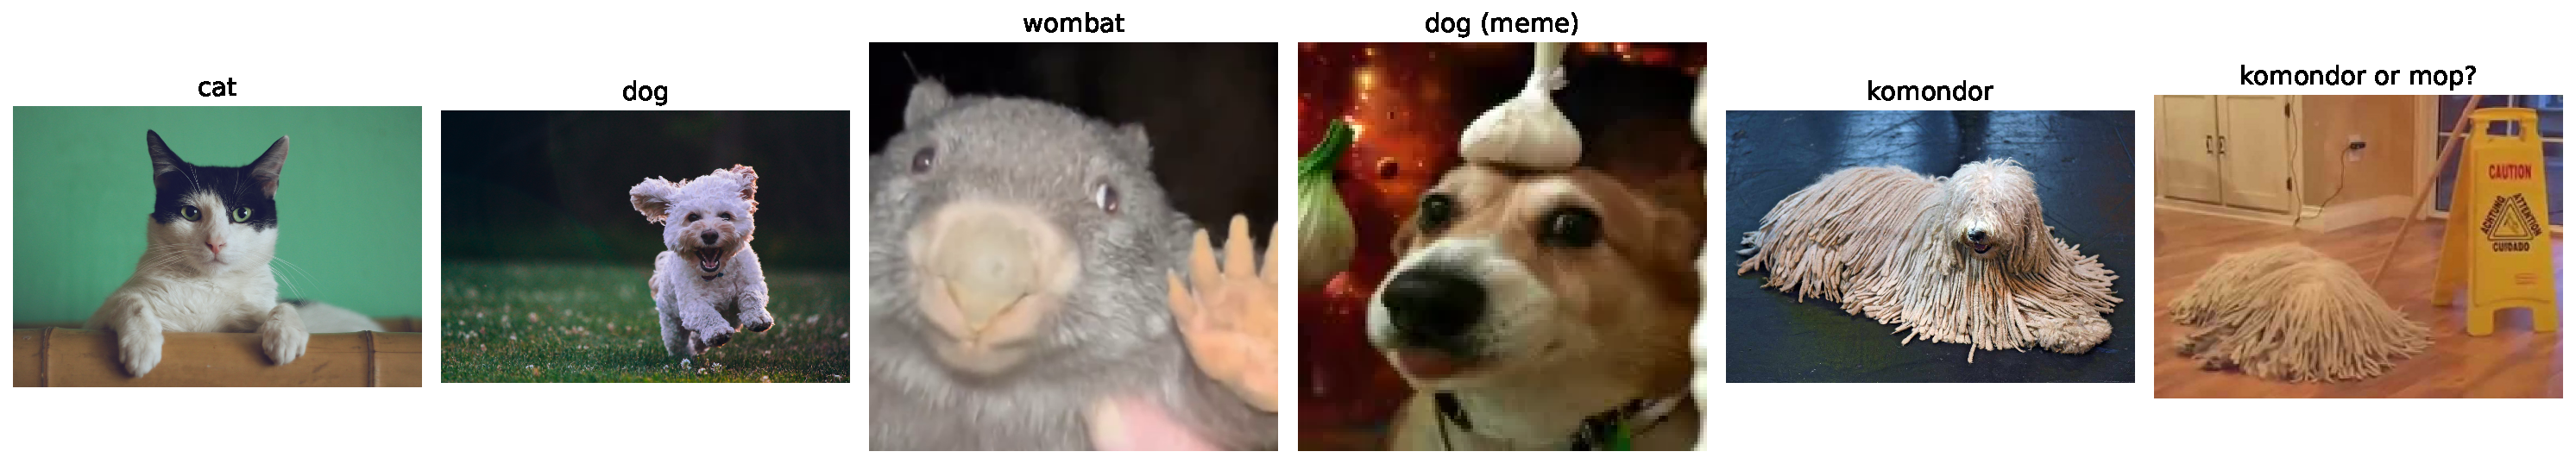
\includegraphics[width=\textwidth]{original_images_vit}
        \caption{}
        \label{subfig:original_images_vit}
    \end{subfigure}
    \begin{subfigure}{0.95\textwidth}
        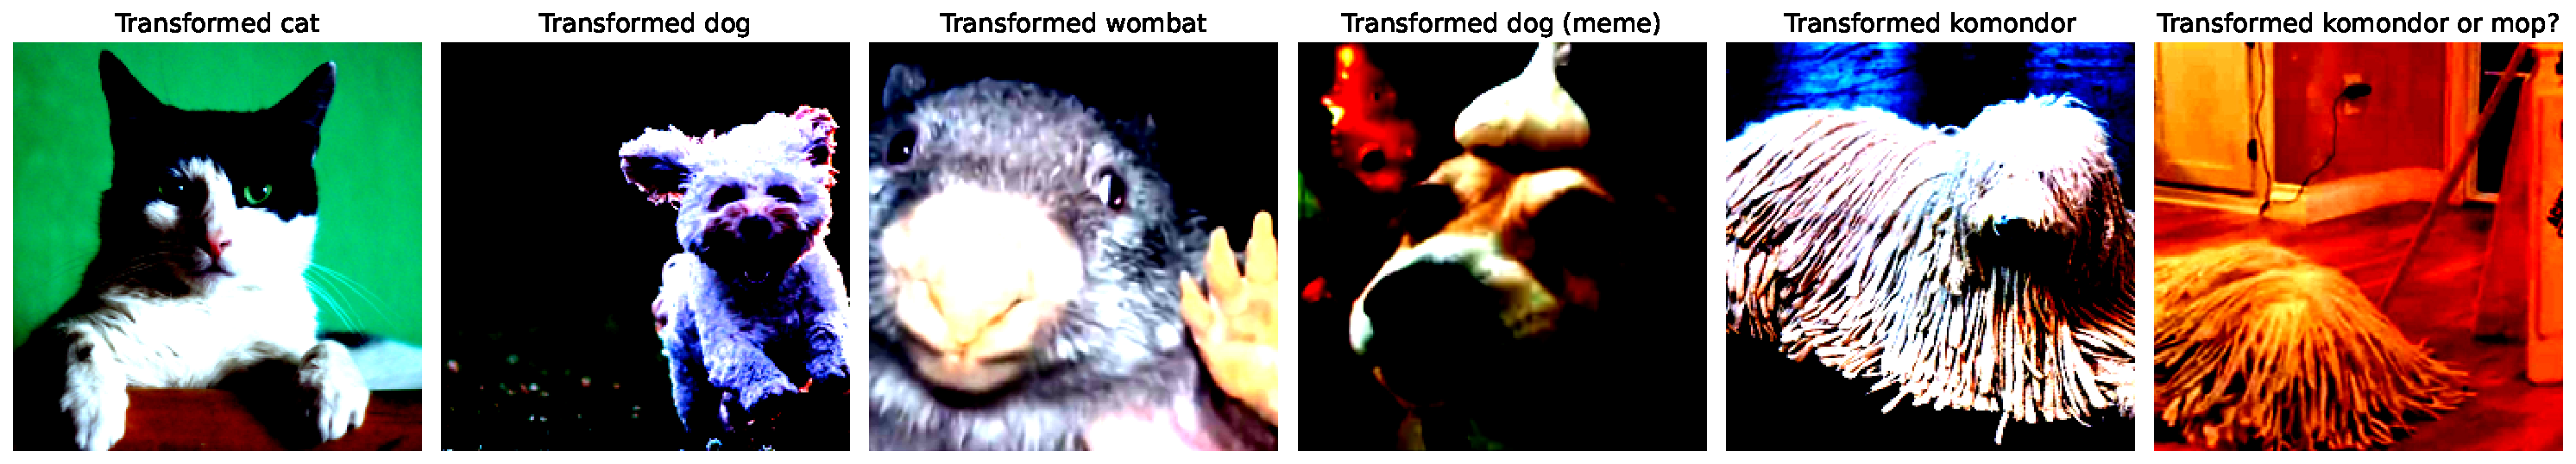
\includegraphics[width=\textwidth]{transformed_images_vit}
        \caption{}
        \label{subfig:transformed_images_vit}
    \end{subfigure}
    \begin{subfigure}{0.95\textwidth}
        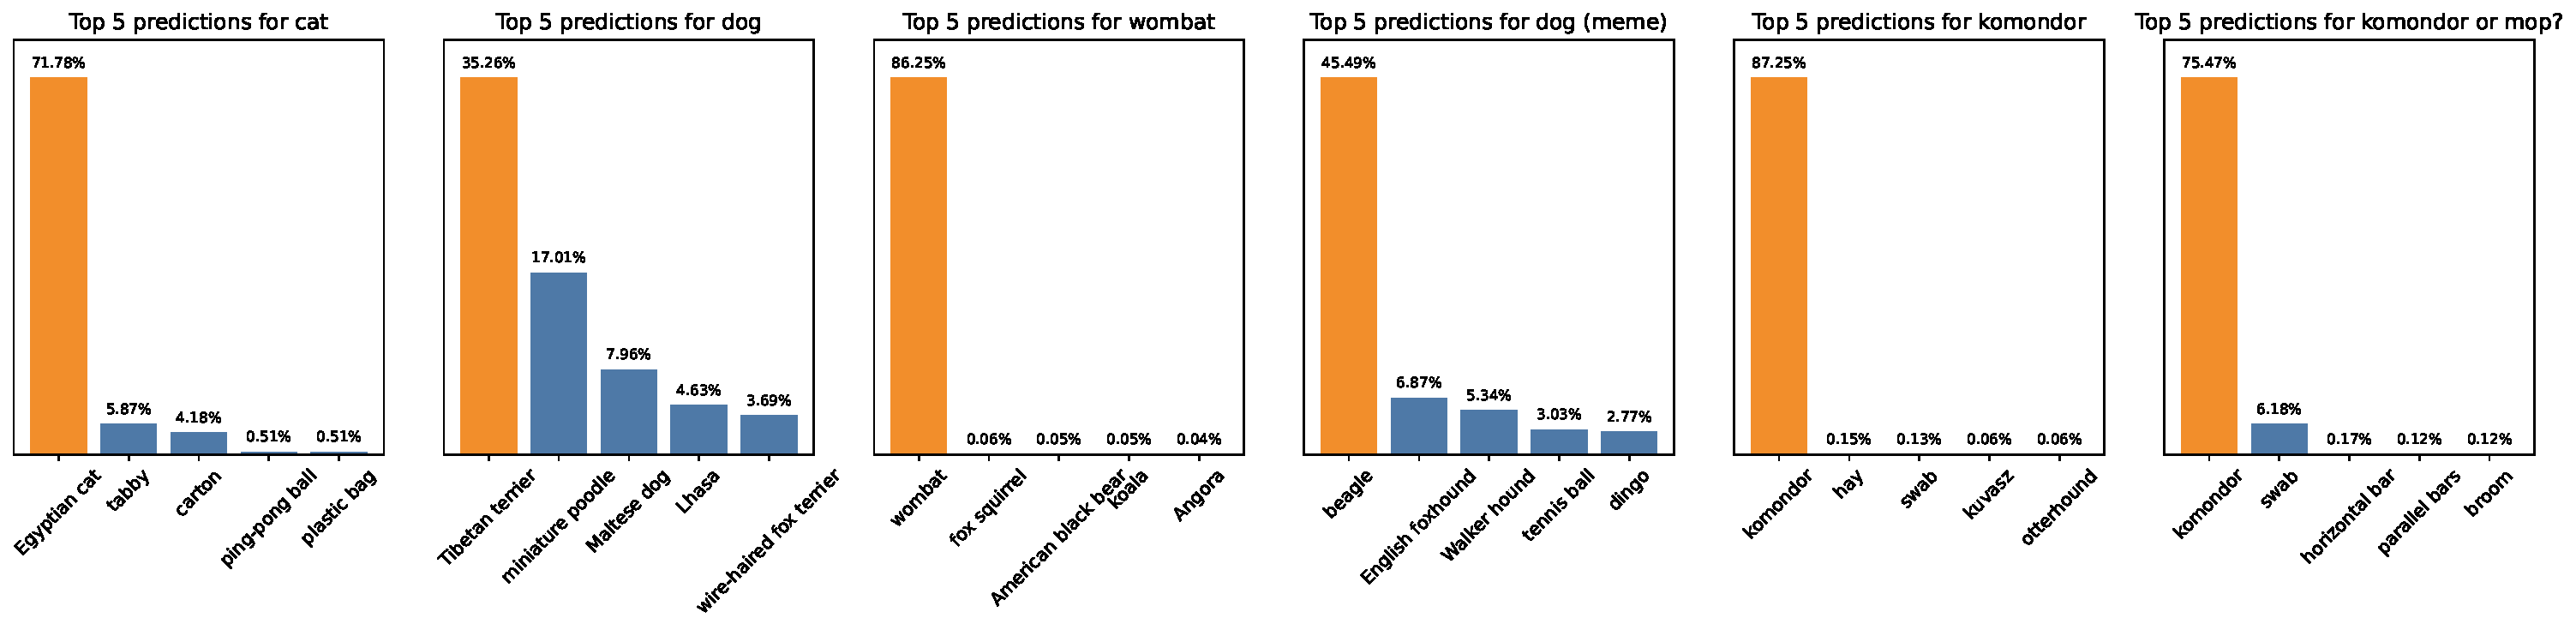
\includegraphics[width=\textwidth]{prediction_plots_vit}
        \caption{}
        \label{subfig:prediction_plots_vit}
    \end{subfigure}
    \caption{Performance evaluation of VisionTransformer pre-trained on ImageNet (IMAGENET1K\_V1 weights): (a) Original images, (b) Transformed images normalized and resized to $224 \times 224$, and (c) Top 5 predicted classes.}
    \label{fig:vit_scratch}
\end{figure}

\begin{figure}[H]
    \centering
    \begin{subfigure}{0.95\textwidth}
        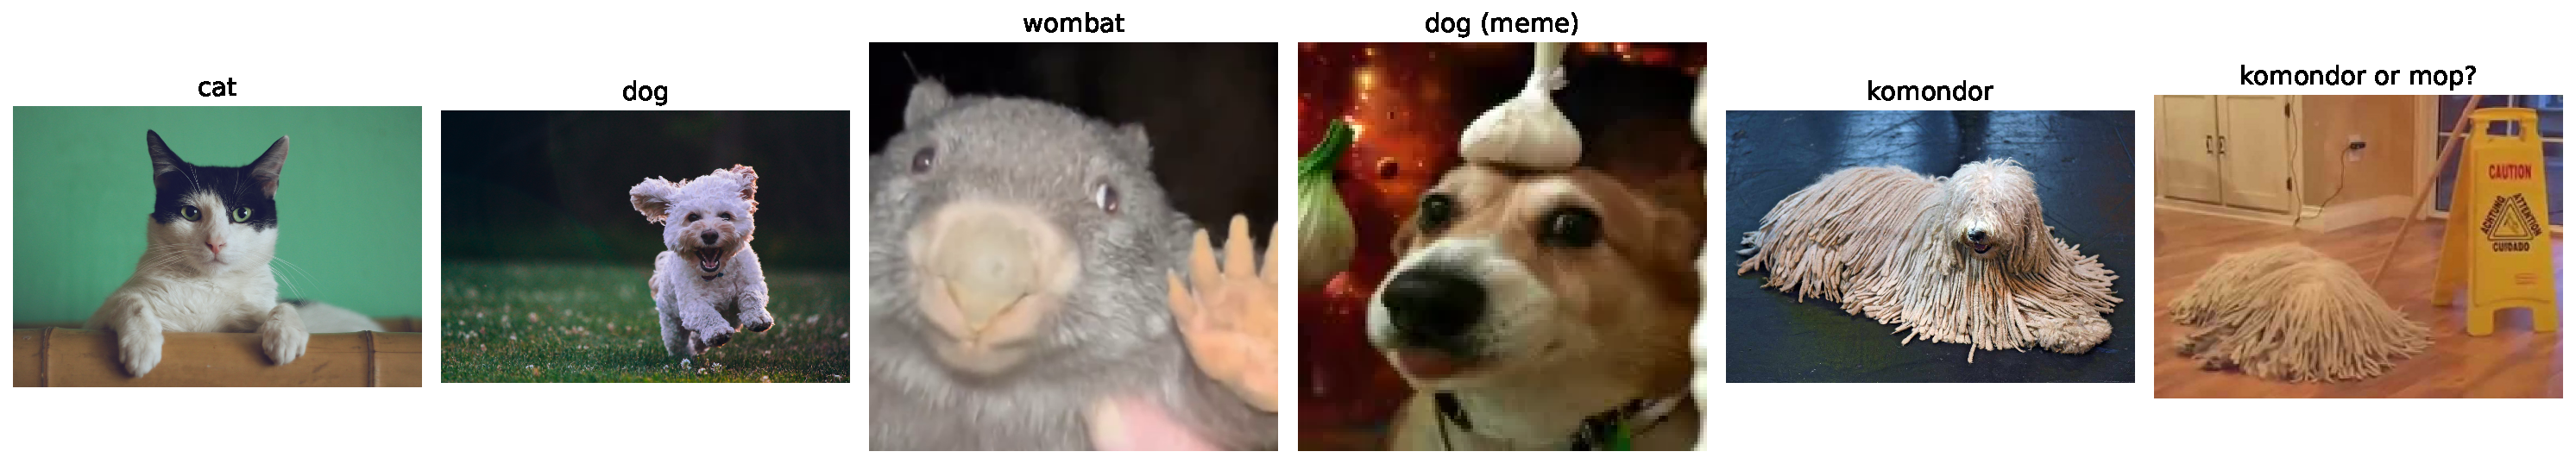
\includegraphics[width=\textwidth]{original_images_vit_bis}
        \caption{}
        \label{subfig:original_images_vit_bis}
    \end{subfigure}
    \begin{subfigure}{0.95\textwidth}
        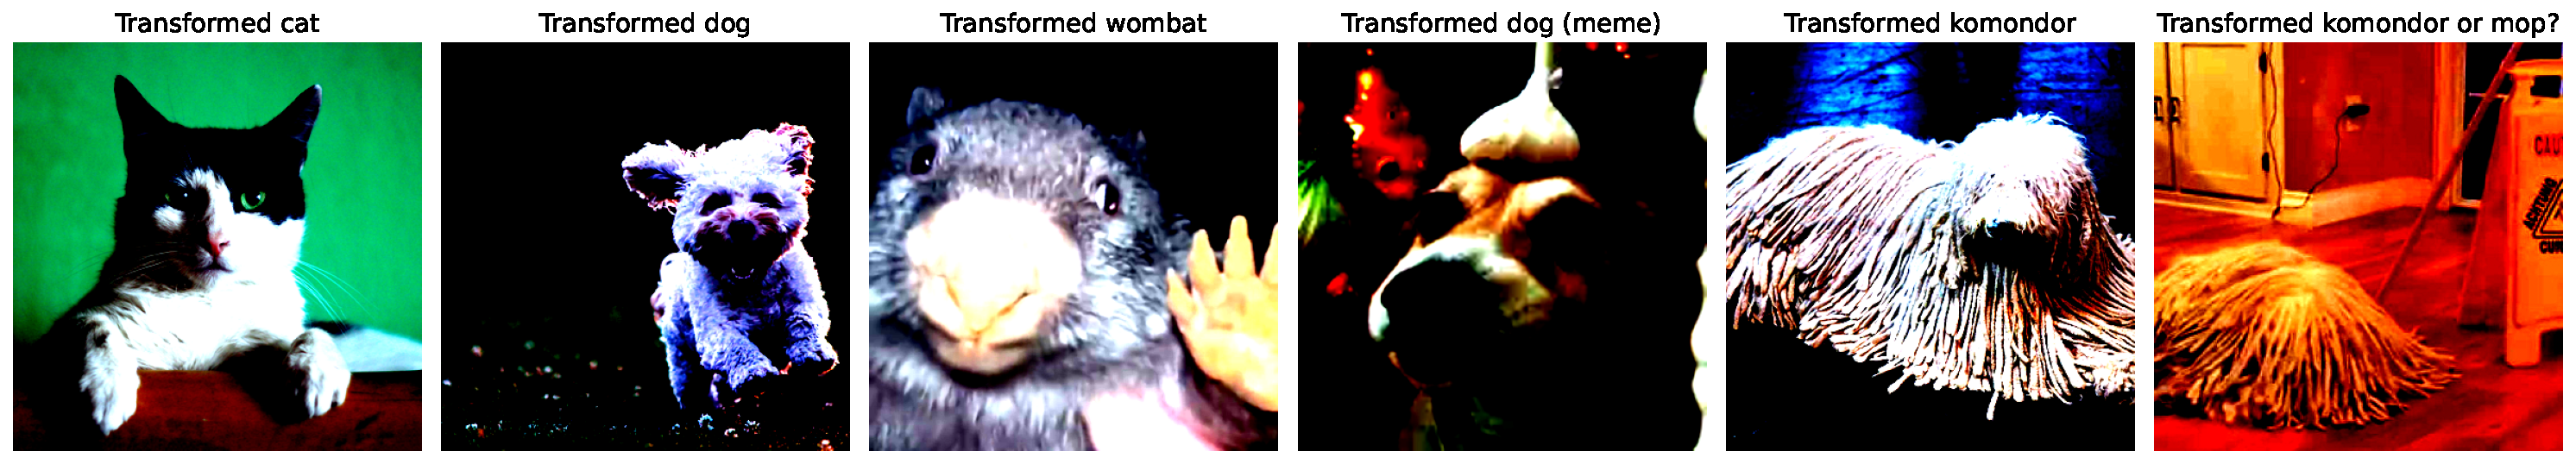
\includegraphics[width=\textwidth]{transformed_images_vit_bis}
        \caption{}
        \label{subfig:transformed_images_vit_bis}
    \end{subfigure}
    \begin{subfigure}{0.95\textwidth}
        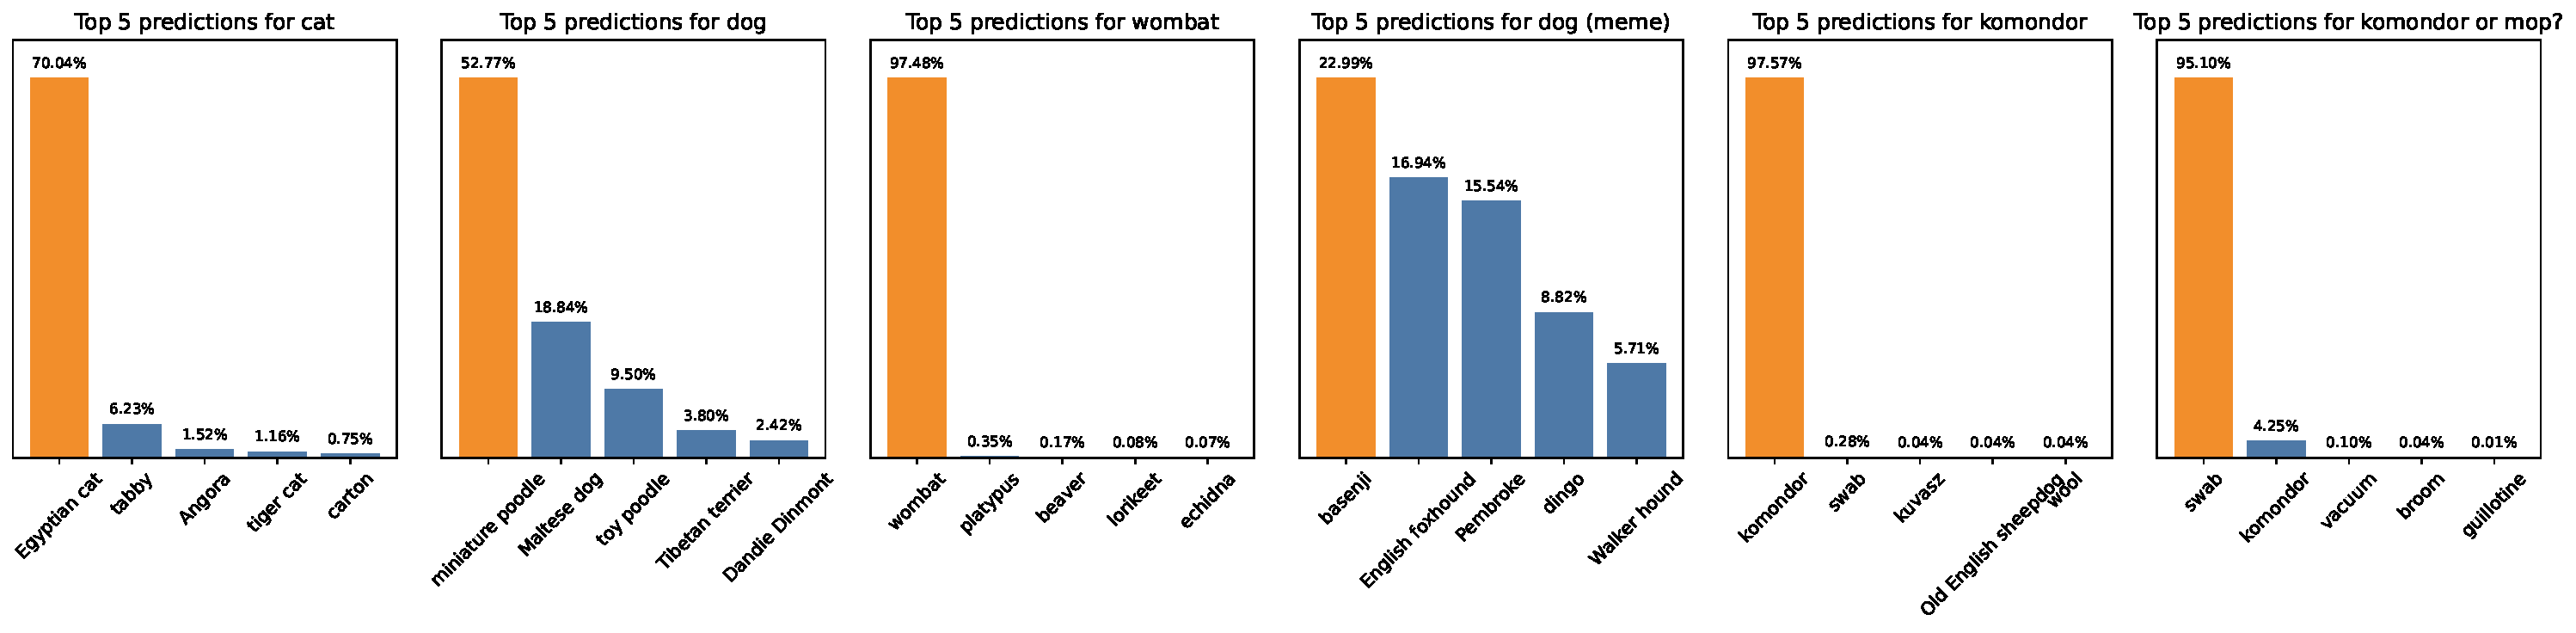
\includegraphics[width=\textwidth]{prediction_plots_vit_bis}
        \caption{}
        \label{subfig:prediction_plots_vit_bis}
    \end{subfigure}
    \caption{Performance evaluation of VisionTransformer pre-trained on ImageNet (IMAGENET1K\_SWAG\_E2E\_V1 weights): (a) Original images, (b) Transformed images normalized and resized to $224 \times 224$, and (c) Top 5 predicted classes.}
    \label{fig:vit_refined}
\end{figure}

\section{Generative Adversarial Networks}
\graphicspath{{figs/2de/}}

\subsection{Longer epochs} \label{appendix:longer_epochs}

\begin{figure}[H]
    \centering

    \begin{subfigure}{0.45\textwidth}
        \centering
        \includegraphics[width=0.95\linewidth]{longer_epochs/lossD.png}
        \caption{}
        \label{subfig:longer_epochs/lossD}
    \end{subfigure}%
    \begin{subfigure}{0.45\textwidth}
        \centering
        \includegraphics[width=0.95\linewidth]{longer_epochs/lossG.png}
        \caption{}
        \label{subfig:longer_epochs/lossG}
    \end{subfigure}

    \begin{subfigure}{0.45\textwidth}
        \centering
        \includegraphics[width=0.95\linewidth]{longer_epochs/D_G_z.png}
        \caption{}
        \label{subfig:longer_epochs/D_G_z}
    \end{subfigure}%
    \begin{subfigure}{0.45\textwidth}
        \centering
        \includegraphics[width=0.95\linewidth]{longer_epochs/D_x.png}
        \caption{}
        \label{subfig:longer_epochs/D_x}
    \end{subfigure}

    \begin{subfigure}{0.45\textwidth}
        \centering
        \includegraphics[width=0.95\linewidth]{longer_epochs/epochs.png}
        \caption{}
        \label{subfig:longer_epochs/epochs}
    \end{subfigure}%

    \caption{Training curves: (a) $loss(D)$, (b) $loss(G)$, (c) $D(G(z))$, (d) $D(x)$ and (e) the number of epochs by the number of iterations.}
    \label{fig:longer_epochs_losses}
\end{figure}

\subsection{Influence of weight initialization.} \label{appendix:init}

\begin{figure}[H]
    \centering

    \begin{subfigure}{0.45\textwidth}
        \centering
        \includegraphics[width=0.95\linewidth]{init/lossD.png}
        \caption{}
        \label{subfig:init/lossD}
    \end{subfigure}%
    \begin{subfigure}{0.45\textwidth}
        \centering
        \includegraphics[width=0.95\linewidth]{init/lossG.png}
        \caption{}
        \label{subfig:init/lossG}
    \end{subfigure}

    \begin{subfigure}{0.45\textwidth}
        \centering
        \includegraphics[width=0.95\linewidth]{init/D_G_z.png}
        \caption{}
        \label{subfig:init/D_G_z}
    \end{subfigure}%
    \begin{subfigure}{0.45\textwidth}
        \centering
        \includegraphics[width=0.95\linewidth]{init/D_x.png}
        \caption{}
        \label{subfig:init/D_x}
    \end{subfigure}

    \begin{subfigure}{0.45\textwidth}
        \centering
        \includegraphics[width=0.95\linewidth]{init/epochs.png}
        \caption{}
        \label{subfig:init/epochs}
    \end{subfigure}%

    \caption{Training curves: (a) $loss(D)$, (b) $loss(G)$, (c) $D(G(z))$, (d) $D(x)$ and (e) the number of epochs by the number of iterations.}
    \label{fig:init_losses}
\end{figure}

\subsection{Influence of learning rate} \label{appendix:gan_lr}

\begin{figure}[H]
    \centering

    \begin{subfigure}{0.45\textwidth}
        \centering
        \includegraphics[width=0.95\linewidth]{lr/lossD.png}
        \caption{}
        \label{subfig:lr/lossD}
    \end{subfigure}%
    \begin{subfigure}{0.45\textwidth}
        \centering
        \includegraphics[width=0.95\linewidth]{lr/lossG.png}
        \caption{}
        \label{subfig:lr/lossG}
    \end{subfigure}

    \begin{subfigure}{0.45\textwidth}
        \centering
        \includegraphics[width=0.95\linewidth]{lr/D_G_z.png}
        \caption{}
        \label{subfig:lr/D_G_z}
    \end{subfigure}%
    \begin{subfigure}{0.45\textwidth}
        \centering
        \includegraphics[width=0.95\linewidth]{lr/D_x.png}
        \caption{}
        \label{subfig:lr/D_x}
    \end{subfigure}

    \begin{subfigure}{0.45\textwidth}
        \centering
        \includegraphics[width=0.95\linewidth]{lr/epochs.png}
        \caption{}
        \label{subfig:lr/epochs}
    \end{subfigure}%

    \caption{Training curves: (a) $loss(D)$, (b) $loss(G)$, (c) $D(G(z))$, (d) $D(x)$ and (e) the number of epochs by the number of iterations.}
    \label{fig:lr_losses}
\end{figure}

\subsection{Influence of $ngf$ and $ndf$} \label{appendix:ngf_ndf}

\begin{figure}[H]
    \centering

    \begin{subfigure}{0.45\textwidth}
        \centering
        \includegraphics[width=0.95\linewidth]{ngf/8/lossD.png}
        \caption{}
        \label{subfig:ngf/8/lossD}
    \end{subfigure}%
    \begin{subfigure}{0.45\textwidth}
        \centering
        \includegraphics[width=0.95\linewidth]{ngf/8/lossG.png}
        \caption{}
        \label{subfig:ngf/8/lossG}
    \end{subfigure}

    \begin{subfigure}{0.45\textwidth}
        \centering
        \includegraphics[width=0.95\linewidth]{ngf/8/D_G_z.png}
        \caption{}
        \label{subfig:ngf/8/D_G_z}
    \end{subfigure}%
    \begin{subfigure}{0.45\textwidth}
        \centering
        \includegraphics[width=0.95\linewidth]{ngf/8/D_x.png}
        \caption{}
        \label{subfig:ngf/8/D_x}
    \end{subfigure}

    \begin{subfigure}{0.45\textwidth}
        \centering
        \includegraphics[width=0.95\linewidth]{ngf/8/epochs.png}
        \caption{}
        \label{subfig:ngf/8/epochs}
    \end{subfigure}%

    \caption{Training curves for $ngf=8$: (a) $loss(D)$, (b) $loss(G)$, (c) $D(G(z))$, (d) $D(x)$ and (e) the number of epochs by the number of iterations.}
    \label{fig:ngf/8_losses}
\end{figure}

\begin{figure}[H]
    \centering

    \begin{subfigure}{0.45\textwidth}
        \centering
        \includegraphics[width=0.95\linewidth]{ngf/128/lossD.png}
        \caption{}
        \label{subfig:ngf/128/lossD}
    \end{subfigure}%
    \begin{subfigure}{0.45\textwidth}
        \centering
        \includegraphics[width=0.95\linewidth]{ngf/128/lossG.png}
        \caption{}
        \label{subfig:ngf/128/lossG}
    \end{subfigure}

    \begin{subfigure}{0.45\textwidth}
        \centering
        \includegraphics[width=0.95\linewidth]{ngf/128/D_G_z.png}
        \caption{}
        \label{subfig:ngf/128/D_G_z}
    \end{subfigure}%
    \begin{subfigure}{0.45\textwidth}
        \centering
        \includegraphics[width=0.95\linewidth]{ngf/128/D_x.png}
        \caption{}
        \label{subfig:ngf/128/D_x}
    \end{subfigure}

    \begin{subfigure}{0.45\textwidth}
        \centering
        \includegraphics[width=0.95\linewidth]{ngf/128/epochs.png}
        \caption{}
        \label{subfig:ngf/128/epochs}
    \end{subfigure}%

    \caption{Training curves for $ngf=128$: (a) $loss(D)$, (b) $loss(G)$, (c) $D(G(z))$, (d) $D(x)$ and (e) the number of epochs by the number of iterations.}
    \label{fig:ngf/128_losses}
\end{figure}

\begin{figure}[H]
    \centering

    \begin{subfigure}{0.45\textwidth}
        \centering
        \includegraphics[width=0.95\linewidth]{ndf/8/lossD.png}
        \caption{}
        \label{subfig:ndf/8/lossD}
    \end{subfigure}%
    \begin{subfigure}{0.45\textwidth}
        \centering
        \includegraphics[width=0.95\linewidth]{ndf/8/lossG.png}
        \caption{}
        \label{subfig:ndf/8/lossG}
    \end{subfigure}

    \begin{subfigure}{0.45\textwidth}
        \centering
        \includegraphics[width=0.95\linewidth]{ndf/8/D_G_z.png}
        \caption{}
        \label{subfig:ndf/8/D_G_z}
    \end{subfigure}%
    \begin{subfigure}{0.45\textwidth}
        \centering
        \includegraphics[width=0.95\linewidth]{ndf/8/D_x.png}
        \caption{}
        \label{subfig:ndf/8/D_x}
    \end{subfigure}

    \begin{subfigure}{0.45\textwidth}
        \centering
        \includegraphics[width=0.95\linewidth]{ndf/8/epochs.png}
        \caption{}
        \label{subfig:ndf/8/epochs}
    \end{subfigure}%

    \caption{Training curves for $ndf=8$: (a) $loss(D)$, (b) $loss(G)$, (c) $D(G(z))$, (d) $D(x)$ and (e) the number of epochs by the number of iterations.}
    \label{fig:ndf/8_losses}
\end{figure}


\begin{figure}[H]
    \centering

    \begin{subfigure}{0.45\textwidth}
        \centering
        \includegraphics[width=0.95\linewidth]{ndf/128/lossD.png}
        \caption{}
        \label{subfig:ndf/128/lossD}
    \end{subfigure}%
    \begin{subfigure}{0.45\textwidth}
        \centering
        \includegraphics[width=0.95\linewidth]{ndf/128/lossG.png}
        \caption{}
        \label{subfig:ndf/128/lossG}
    \end{subfigure}

    \begin{subfigure}{0.45\textwidth}
        \centering
        \includegraphics[width=0.95\linewidth]{ndf/128/D_G_z.png}
        \caption{}
        \label{subfig:ndf/128/D_G_z}
    \end{subfigure}%
    \begin{subfigure}{0.45\textwidth}
        \centering
        \includegraphics[width=0.95\linewidth]{ndf/128/D_x.png}
        \caption{}
        \label{subfig:ndf/128/D_x}
    \end{subfigure}

    \begin{subfigure}{0.45\textwidth}
        \centering
        \includegraphics[width=0.95\linewidth]{ndf/128/epochs.png}
        \caption{}
        \label{subfig:ndf/128/epochs}
    \end{subfigure}%

    \caption{Training curves for $ndf=128$: (a) $loss(D)$, (b) $loss(G)$, (c) $D(G(z))$, (d) $D(x)$ and (e) the number of epochs by the number of iterations.}
    \label{fig:ndf/128_losses}
\end{figure}

\subsection{Trying CIFAR-10 dataset.} \label{appendix:cifar10_32}

\begin{figure}[H]
    \centering

    \begin{subfigure}{0.45\textwidth}
        \centering
        \includegraphics[width=0.95\linewidth]{cifar10/32/lossD.png}
        \caption{}
        \label{subfig:cifar10/32/lossD}
    \end{subfigure}%
    \begin{subfigure}{0.45\textwidth}
        \centering
        \includegraphics[width=0.95\linewidth]{cifar10/32/lossG.png}
        \caption{}
        \label{subfig:cifar10/32/lossG}
    \end{subfigure}

    \begin{subfigure}{0.45\textwidth}
        \centering
        \includegraphics[width=0.95\linewidth]{cifar10/32/D_G_z.png}
        \caption{}
        \label{subfig:cifar10/32/D_G_z}
    \end{subfigure}%
    \begin{subfigure}{0.45\textwidth}
        \centering
        \includegraphics[width=0.95\linewidth]{cifar10/32/D_x.png}
        \caption{}
        \label{subfig:cifar10/32/D_x}
    \end{subfigure}

    \begin{subfigure}{0.45\textwidth}
        \centering
        \includegraphics[width=0.95\linewidth]{cifar10/32/epochs.png}
        \caption{}
        \label{subfig:cifar10/32/epochs}
    \end{subfigure}%

    \caption{Training curves: (a) $loss(D)$, (b) $loss(G)$, (c) $D(G(z))$, (d) $D(x)$ and (e) the number of epochs by the number of iterations.}
    \label{fig:cifar10_32_curves}
\end{figure}

\subsection{Generating higher resolution images on CIFAR-10.} \label{appendix:cifar10_64}

\begin{figure}[H]
    \centering

    \begin{subfigure}{0.45\textwidth}
        \centering
        \includegraphics[width=0.95\linewidth]{cifar10/64_nz100/lossD.png}
        \caption{}
        \label{subfig:cifar10/64_nz100/lossD}
    \end{subfigure}%
    \begin{subfigure}{0.45\textwidth}
        \centering
        \includegraphics[width=0.95\linewidth]{cifar10/64_nz100/lossG.png}
        \caption{}
        \label{subfig:cifar10/64_nz100/lossG}
    \end{subfigure}

    \begin{subfigure}{0.45\textwidth}
        \centering
        \includegraphics[width=0.95\linewidth]{cifar10/64_nz100/D_G_z.png}
        \caption{}
        \label{subfig:cifar10/64_nz100/D_G_z}
    \end{subfigure}%
    \begin{subfigure}{0.45\textwidth}
        \centering
        \includegraphics[width=0.95\linewidth]{cifar10/64_nz100/D_x.png}
        \caption{}
        \label{subfig:cifar10/64_nz100/D_x}
    \end{subfigure}

    \begin{subfigure}{0.45\textwidth}
        \centering
        \includegraphics[width=0.95\linewidth]{cifar10/64_nz100/epochs.png}
        \caption{}
        \label{subfig:cifar10/64_nz100/epochs}
    \end{subfigure}%

    \caption{Training curves: (a) $loss(D)$, (b) $loss(G)$, (c) $D(G(z))$, (d) $D(x)$ and (e) the number of epochs by the number of iterations.}
    \label{fig:cifar10_64_nz100_curves}
\end{figure}

\subsection{Conditional GAN.} \label{appendix:cDCGAN}

\begin{figure}[H]
    \centering

    \begin{subfigure}{0.45\textwidth}
        \centering
        \includegraphics[width=0.95\linewidth]{cDCGAN/lossD.png}
        \caption{}
        \label{subfig:cDCGAN/lossD}
    \end{subfigure}%
    \begin{subfigure}{0.45\textwidth}
        \centering
        \includegraphics[width=0.95\linewidth]{cDCGAN/lossG.png}
        \caption{}
        \label{subfig:cDCGAN/lossG}
    \end{subfigure}

    \begin{subfigure}{0.45\textwidth}
        \centering
        \includegraphics[width=0.95\linewidth]{cDCGAN/D_G_z.png}
        \caption{}
        \label{subfig:cDCGAN/D_G_z}
    \end{subfigure}%
    \begin{subfigure}{0.45\textwidth}
        \centering
        \includegraphics[width=0.95\linewidth]{cDCGAN/D_x.png}
        \caption{}
        \label{subfig:cDCGAN/D_x}
    \end{subfigure}

    \begin{subfigure}{0.45\textwidth}
        \centering
        \includegraphics[width=0.95\linewidth]{cDCGAN/epochs.png}
        \caption{}
        \label{subfig:cDCGAN/epochs}
    \end{subfigure}%

    \caption{Training curves: (a) $loss(D)$, (b) $loss(G)$, (c) $D(G(z))$, (d) $D(x)$ and (e) the number of epochs by the number of iterations.}
    \label{fig:cDCGAN_curves}
\end{figure}


\end{document}